\documentclass[12pt, a4paper]{book}%, oneside

\usepackage[headings]{fullpage}
\usepackage{setspace}
% ---- Added for this thesis: encoding, maths, long tables, special characters, URLs ----
\usepackage[T1]{fontenc}
\usepackage[utf8]{inputenc}
\usepackage{lmodern}
\usepackage{amsmath,amssymb}
\usepackage{longtable,calc}
\usepackage{etoolbox}
\makeatletter
\patchcmd\longtable{\par}{\if@noskipsec\mbox{}\fi\par}{}{}
\makeatother
\usepackage{footnotehyper}
\makesavenoteenv{longtable}
\usepackage{xcolor}
\usepackage{fvextra}
\fvset{breaklines=true}
\usepackage{newunicodechar}
\newunicodechar{†}{$\dagger$}\newunicodechar{κ}{$\kappa$}\newunicodechar{≥}{$\geq$}\newunicodechar{≤}{$\leq$}\newunicodechar{→}{$\rightarrow$}\newunicodechar{↔}{$\leftrightarrow$}\newunicodechar{±}{$\pm$}\newunicodechar{✔}{Y}\newunicodechar{≠}{$\neq$}
\providecommand{\tightlist}{\setlength{\itemsep}{0pt}\setlength{\parskip}{0pt}}
\setlength{\emergencystretch}{3em}
\renewcommand{\arraystretch}{1.15}
\usepackage{xurl}
% ---- end of additions ----

% \usepackage[top=1.5cm,right=1.5cm,bottom=1.5cm,left=1.5cm]{geometry}
% \usepackage{fancyhdr}
% \setlength{\headheight}{20pt} 
% \usepackage{graphics}
\usepackage{graphicx}
\graphicspath{{figures/}} % added: screenshots live in figures/
\usepackage{float}
\usepackage{tikz}
\usetikzlibrary{positioning,arrows.meta,fit,backgrounds}
\usepackage{pgfplots}
\pgfplotsset{compat=1.18}
\usepackage{subfig}
\usepackage{array}
% \usepackage{xtab}
\usepackage{multirow}
\usepackage{booktabs}
\usepackage{appendix}
\usepackage[pdfborder={0 0 0}, colorlinks=true, linkcolor=black, citecolor=blue, urlcolor=blue]{hyperref}
% printonlyused removed: the list of abbreviations is printed in full; nohyperlinks avoids broken links
\usepackage[nohyperlinks]{acronym}
\usepackage{algorithmic}
\usepackage{algorithm}
\usepackage{ifpdf}
% \setlength{\parindent}{0pt}

\newcommand{\submissionDay}{5}
\newcommand{\submissionMonth}{January}
\newcommand{\submissionYear}{2027}
\newcommand{\submissionDate}{\submissionDay~\submissionMonth,~\submissionYear}
\newcommand{\typeOfThesis}{Bachelor Thesis}

\newcommand{\titleOfThesisOne}{JadwAI: AI-Assisted University Timetabling Through Natural-Language Constraint Extraction}

\newcommand{\authorOfThesis}{Rawda Yassin}
\newcommand{\supervisorOne}{Dr. John Zaki}
\newcommand{\supervisorTwo}{}
\newcommand{\supervisorThree}{}

\newcommand{\includefig}[4]{
    \begin{figure}[ht]
     \centering
      \includegraphics[width=#1\textwidth]{images/#2}
      \caption{#3}
      \label{#4}
    \end{figure}
}

\newcommand{\includefigWSC}[5]{
    \begin{figure}[ht]
     \centering
      \includegraphics[width=#1\textwidth]{images/#2}
      \caption[#3]{#4}
      \label{#5}
    \end{figure}
}

\newcommand{\includeeps}[4]{
\includefig{#1}{#2.eps}{#3}{#4}
}

\newcommand{\includeepsWSC}[5]{
\includefigWSC{#1}{#2.eps}{#3}{#4}{#5}
}


\ifpdf
\pdfinfo {
	/Author (\authorOfThesis)
	/Title (\titleOfThesisOne)
	/Subject (\typeOfThesis)
	/Keywords ()
	/CreationDate (D:20090707085533)
}
\fi

\begin{document}
% \overfullrule=5pt
\pagestyle{plain}
\pagenumbering{Roman}

\newcommand{\titlePage}{

\thispagestyle{empty}
\begin{center}
	
\includegraphics[width=3.5cm]{figures/giu_logo.png}\\[2mm]
	\textbf{German International University}\\[2mm]
		% NOTE: check the exact faculty name (old draft said "ICS - Software Engineering")
		\textbf{Faculty of Informatics and Computer Science}\\[1mm]

	
	\vspace{2cm}
	\doublespacing
	{\Huge \textbf{\titleOfThesisOne}}\\
	\singlespacing
	\vspace{2cm}
	{\large \textbf{\typeOfThesis}}\\
	
	\vfill
	\parbox{1cm}{
  		\begin{large}
    			\begin{tabbing}
       			Author: \hspace{2cm}  
        			\=\authorOfThesis\\[2mm]
      			Supervisor: 
        			\>\supervisorOne\\[2mm]
      			Submission Date: 
        			\>\submissionDate\\
    			\end{tabbing}
  		\end{large}
	}\\
\end{center}
\clearpage
}
%++++++++++++++++++++++++++++++++++++++++++++++++++++++++++++++++++++
\titlePage
\thispagestyle{empty}\ \clearpage
\titlePage
%++++++++++++++++++++++++++++++++++++++++++++++++++++++++++++++++++++
\thispagestyle{empty}
This is to certify that:
\begin{itemize}
\item[(i)] the thesis comprises only my original work toward the Bachelor Degree
\item[(ii)] due acknowledgement has been made in the text to all other material used
\end{itemize}

\vspace{2cm}
\begin{flushright}
\rule[0mm]{6cm}{0.2mm}\\
\authorOfThesis\\
\submissionDay~\submissionMonth,~\submissionYear\\
\end{flushright}
\clearpage


\chapter*{Acknowledgments}
\addcontentsline{toc}{chapter}{Acknowledgments}
\label{chap:ack}
% TO WRITE, in your own words: supervisor, anyone who helped, and any funding.
[Acknowledgments to be written.]


\chapter*{Abstract}
% \addcontentsline{toc}{chapter}{Abstract}
\label{chap:abstract}
% NOTE (24 Nov 2026): First draft (about 290 words) written from the Results and Conclusion chapters at the owner's request, drafted with AI assistance; reword in your own words before submission. Structure: why and aim; what was built and evaluated with the main results; what was concluded.

University timetables depend on many rules about when instructors, rooms and student groups are available. Administrators usually state these rules informally, and entering them into a timetabling system through forms is slow. This thesis investigates whether a language model can turn such requirements, written in English, formal Arabic, Egyptian Arabic or a mix of them, into formal rules for a constraint solver without allowing a wrong interpretation to reach a published timetable.

The work produced JadwAI, a web application for teaching and examination timetables. Requirements are interpreted into a closed set of rules, shown to the administrator for approval, and only approved rules are passed to a CP-SAT solver. Every generated timetable is checked by an independent validator before it can be published. The system also includes JAI, a chat assistant whose language model runs locally. On a synthetic development corpus of 144 statements, a rule-based parser produced the exact expected output for 32.6\% of statements. A local seven-billion-parameter model reached 9.0\% with the application's prompt and 16.7\% with a prompt aligned to the evaluation contract, and its intervals overlapped the parser's. The model learned to ask for missing information, but also asked when it was not needed and missed every conflict. The assistant model was fine-tuned in four rounds; guide-grounded training answers improved it in a blind rating, while one round made it worse. The solver built a validated department timetable of 448 sessions and a university-scale timetable of 2{,}703 sessions in six parts.

The results suggest that, at this scale, a local language model is useful as a proposer whose output is reviewed and validated, not as a trusted interpreter. The labels are unreviewed and the corpus is synthetic, so the findings are development evidence only; the comparison with manual entry remains future work.

\tableofcontents
% \addcontentsline{toc}{chapter}{Contents}
\clearpage 

\pagestyle{headings}
\pagenumbering{arabic}

% \setlength\parskip{15pt}
\setlength\parskip{.5\baselineskip plus .2\baselineskip
	minus .4\baselineskip}
% \setlength\parskip{.5\baselineskip \@plus .1\baselineskip \@minus ..1\baselineskip}


% NOTE (migration 23 Nov 2026): Text moved unchanged from main.tex. Much of it was drafted with AI assistance; rewrite it in your own words before submission (the supervisor runs AI checks).
% NOTE (23 Nov 2026): Research questions, scope, contributions and organisation updated to match the rewritten Methodology. RQ3/RQ4 reframing assumes the supervisor accepts RQ-EVIDENCE.md; change it together with Methodology Section 3.1 otherwise.
\hypertarget{introduction}{%
\chapter{Introduction}\label{introduction}}


\hypertarget{problem-statement}{%
\section{Problem statement}\label{problem-statement}}

Administrators must record scheduling requirements accurately enough to protect access to required teaching while accommodating staff availability and suitable facilities. If the system misunderstands a requirement, a timetable can appear acceptable while failing the intended institutional need. The practical problem is therefore how to support clear requirement entry, useful clarification, and informed approval without adding excessive administrative effort.

The five reviewed timetabling papers provide evidence about scheduling needs and capabilities, but do not evaluate ordinary-language requirement entry with this review workflow. This thesis investigates that task within a limited timetabling scope. Its gap claim is bounded by the reviewed sources; a wider documented literature search remains planned.

\hypertarget{research-gap}{%
\section{Research gap}\label{research-gap}}

Within the five retained timetabling papers, constraint acquisition is a developer or
administrator task and is not evaluated as a research problem (Chapter~\ref{literature-review}). The additional LLM-related sources verified so far address
different questions: LLMs solving scheduling problems described in text
\cite{sharma2026schedbench}, a pilot on appliance scheduling in Italian
\cite{sanguinetti2025preferences}, and a benchmark of LLMs writing constraint
models from problem descriptions~\cite{michailidis2025cpbench},
whose task differs because the output is a general constraint program
with no institutional data to resolve against and no review step. The
gap addressed here is therefore the \emph{evaluation of
natural-language-to-constraint extraction for university course
timetabling}, with human review and independent validation, using a
fixed formal model so that extraction quality can be separated from
solver behaviour. The novelty claim is limited to this evaluated
combination; the use of an LLM is not itself claimed to be novel.

\hypertarget{research-questions}{%
\section{Research questions}\label{research-questions}}

\begin{itemize}
\tightlist
\item
  \textbf{RQ1 (primary).} How accurately can an LLM extract formal
  university scheduling constraints from natural-language requirements
  --- including entity references, parameters and hard/soft
  classification --- when output is restricted to a closed constraint
  vocabulary?
\item
  \textbf{RQ2.} Can the system identify ambiguous, missing,
  contradictory or unsupported requirements and request useful
  clarification instead of guessing?
\item
  \textbf{RQ3.} Does AI-assisted constraint entry with human review
  reduce entry time and the number of corrections compared with manual
  form entry while preserving correct interpretation?
\item
  \textbf{RQ4.} How does a locally hosted base language model compare
  with the same model fine-tuned on reviewed, guide-grounded examples,
  in answer quality and latency, on the same held-out cases?
\end{itemize}

RQ1 and RQ2 are evaluated overall and separately for English, formal Arabic, Egyptian Arabic and mixed Arabic/English, by comparing a rule-based parser with a locally hosted language model on development data with draft labels. The results are therefore development-level evidence, not a confirmatory held-out result. RQ3 could not be studied, because no participants or ethics approval were available in the project period; it is discussed as future work. RQ4 originally compared several commercial models; because no budget for paid calls was approved, it compares a local base model with its fine-tuned versions (Chapter~\ref{methodology-proposed-study}).

A supporting engineering question concerns whether the surrounding
system can keep the model honest: \emph{can an independent validator and
an approval workflow ensure that only reviewed constraints reach the
solver and that no schedule with a supported hard-rule violation is
published?} This is verified by testing
(Section~\ref{scheduling-validation-and-system-behaviour-evaluation}), not by statistical inference.

\hypertarget{objectives}{%
\section{Objectives}\label{objectives}}

\begin{enumerate}
\def\labelenumi{\arabic{enumi}.}
\tightlist
\item
  Identify and document the supported educational and administrative scheduling requirements.
\item
  Enable administrators to enter requirements in ordinary language, inspect their interpretation, and clarify or correct them before approval.
\item
  Generate candidate course timetables that respect approved attendance, availability and facility requirements.
\item
  Give administrators understandable checks and feedback for generated timetables and manual changes before publication.
\item
  Evaluate interpretation correctness separately from timetable quality, and evaluate the local assistant model before and after fine-tuning.
\item
  Deliver a working prototype, reproducible evaluation records and this thesis.
\end{enumerate}

\hypertarget{contribution-proportional-to-the-evidence}{%
\section{Contribution (proportional to the
evidence)}\label{contribution-proportional-to-the-evidence}}

The contributions are: (i) a documented set of supported rules and a
machine-readable output contract for timetabling requirements, with
explicit decisions for clarification, unsupported and conflicting
requests; (ii) a synthetic development corpus of 144 statements in four
language categories with a versioned annotation guide, whose labels are
draft and unreviewed; (iii) a development-level comparison of a
rule-based parser and a locally hosted language model on that corpus,
with family-level uncertainty; (iv) a fine-tuning study of a local
assistant model in four rounds, including a round that made it worse
and the reason; and (v) a working prototype for teaching and examination
timetables in which an approval workflow and an independent validator
keep unreviewed or invalid output from being used. No claim is made
about accuracy on real administrators' statements or about reduced
administrative effort.

\hypertarget{scope}{%
\section{Scope}\label{scope}}

\textbf{Project scope:} JadwAI supports course timetabling for one semester at a time, using a repeating weekly pattern, from a single department up to a whole university built in parts. Lectures, tutorials and laboratories have durations and weekly occurrences; student groups are the unit of student-conflict checking. Natural-language requirements in English, formal Arabic, Egyptian Arabic and mixed Arabic/English are part of the core research scope, alongside an English/Arabic interface with right-to-left presentation. JAI (pronounced ``jay'') is the website's chat assistant; its language model runs on the same server as the application.

The solver chooses instructors, times and rooms. Eligibility is recorded separately for lecture, tutorial and laboratory activities. Each activity retains one instructor across its weekly occurrences; instructor, time and room assignments may be locked. Mandatory weekly instructor workload limits and daily limits for instructors and groups are supported. The unit is elapsed teaching hours: a 90-minute session contributes 1.5 hours, counted once per instructor irrespective of how many groups attend; fixed breaks are excluded. Configured weekly instructor maxima and global hard daily caps are implemented. Preferred daily-limit variants and entity-specific daily overrides are not implemented.

\textbf{Added during the project:} examination timetabling (quizzes, midterms and finals, with halls and TA invigilators), repair suggestions for impossible timetables (proposed to the administrator, never applied automatically), and generation in parts for university-scale data. \textbf{Deferred extensions:} individual enrolments, minimal-change regeneration, calendar feeds and notifications. \textbf{Excluded:} native mobile applications, attendance, payroll, full student-information-system integration, automated registration or sectioning, and institution-wide production deployment. The implementation status of each requirement is listed in Appendix~\ref{app:requirements}.

\hypertarget{organisation-of-the-thesis}{%
\section{Organisation of the thesis}\label{organisation-of-the-thesis}}

Chapter~\ref{chap:background} introduces university timetabling and the constraint-entry problem. Chapter~\ref{literature-review} reviews five timetabling papers through educational needs, implemented capabilities and reported evidence, and examines a study of natural-language preference interpretation. Chapter~\ref{methodology-proposed-study} describes the method followed: the research design, the interpretation contract, the development corpus, the methods compared, the metrics, the fine-tuning of the assistant model, the engineering verification, and the threats to validity. Chapter~\ref{chap:implementation} describes the implemented system and the JAI assistant. Chapter~\ref{evidence} reports the measurements, and Chapter~\ref{chap:conclusion} summarises the findings, limitations and future work. The appendices list the requirements, screenshots of the prototype, and the project timeline with traceability to the requirements.

\chapter{Background}\label{chap:background}

% NOTE (24 Nov 2026): Rewritten and extended with sources at the owner's request (drafted with AI assistance; reword in your own words before submission). Every new reference was checked against arXiv, publisher or catalogue records on 24 Nov 2026.

This chapter introduces the concepts the rest of the thesis relies on: university timetabling, the step of turning requirements into formal rules, constraint programming and the CP-SAT solver, large language models and structured output, running and fine-tuning a model locally, and Arabic text in software.

\section{University timetabling}\label{university-timetabling}

University timetabling assigns teaching activities to times, rooms and instructors so that students can attend what they are required to attend and staff can teach within the available time and facilities. These are educational and administrative problems before they are computational ones: an overlapping required lecture prevents attendance, and an unsuitable room prevents a planned laboratory. Two related problems are usually distinguished~\cite{schaerf1999survey,petrovic2004university}. \emph{Course timetabling} places repeated weekly lectures, tutorials and laboratories. \emph{Examination timetabling} places one-off assessments on dates, with different rules for halls, spacing and clashes.

Both problems are combinatorial: the number of possible timetables grows very quickly with the number of sessions, rooms and periods, and finding a good one is computationally hard in general~\cite{schaerf1999survey}. Practical systems therefore use search methods such as local search, integer programming or constraint programming, and they are judged on real institutional data rather than on proofs of optimality~\cite{muller2025itc}.

Rules are usually divided into two kinds. A \emph{hard} (mandatory) constraint must hold in every acceptable timetable, for example ``no student group has two sessions at the same time''. A \emph{soft} (preferred) constraint describes a desirable arrangement, for example a preferred teaching period. Breaking a soft constraint adds a penalty, and the timetable with the lowest total penalty is preferred. Which rules are hard and how soft penalties are weighted is an institutional decision, not a technical one.

The timetabling papers reviewed in Chapter~\ref{literature-review} show different priorities. Sobh, Cousens and Patel~\cite{sobh_course_scheduler} focus on offering course combinations that satisfy degree requirements. Müller, Rudová and Müllerová~\cite{muller2025itc} describe compatible lectures, seminars and laboratories, including travel between buildings. Abdennadher and Edward~\cite{abdennadher_guc_exams} consider examination clashes, retakes and spacing at the German University in Cairo. Kaya~\cite{kaya2026drl} addresses examination scheduling across several campuses. None of them assumes that a clash-free timetable improves learning by itself; it is a precondition for access.

\section{The constraint-entry problem}\label{the-constraint-entry-problem}

A solver needs explicit rules: which entity, which day and time, how strict, and with what weight. Administrators state requirements informally, often several in one sentence. ``Dr Ahmed cannot teach on Tuesdays and prefers morning classes'' contains a hard unavailability and a soft preference, and ``morning'' has no meaning to a solver until the institution defines it. A wrong reading --- treating the preference as mandatory, choosing the wrong Ahmed, or inventing a definition of ``morning'' --- produces a timetable that satisfies the formal model and still fails the administrator's intention. A valid timetable is therefore no evidence that the rules were understood correctly.

In the reviewed systems this translation is done by people and is not itself studied. Constraints are written by developers as declarative programs~\cite{abdennadher_guc_exams}, supplied in benchmark formats~\cite{muller2025itc}, formalised by researchers for one institution~\cite{kaya2026drl}, set as weights by a timetable officer~\cite{petrovic2004university}, or chosen by instructors as time slots~\cite{sobh_course_scheduler}. Form-based entry is precise but slow. An informal walkthrough of the public UniTime demonstration on 4 October 2026 illustrates the effort: recording that one instructor prefers no teaching after 3~PM meant opening the instructor's preferences, choosing a strength and marking 15 half-hour cells over five days. This single observation on sample data motivates the project; it is not evidence about any deployed system.

\section{Constraint programming and CP-SAT}\label{bg-cp}

Constraint programming describes a problem as \emph{variables}, each with a finite set of possible values, and \emph{constraints} that restrict which combinations of values are allowed~\cite{rossi2006handbook}. A solver searches for an assignment that satisfies every constraint. While it searches, it uses \emph{propagation}: each constraint removes values that can no longer lead to a solution, which prunes large parts of the search space. Many problems also have an \emph{objective} to minimise, such as the total soft-constraint penalty.

Scheduling is a natural fit. A session can be an \emph{interval variable} with a start and a length, and a single \emph{no-overlap} constraint states that the intervals assigned to one room, instructor or group never overlap~\cite{rossi2006handbook}. This is much smaller than a model with one yes/no variable for every combination of session, time, room and instructor.

JadwAI uses CP-SAT, the constraint solver in Google OR-Tools~\cite{google_cpsat}. CP-SAT combines constraint propagation with techniques from Boolean satisfiability solving and can run several search strategies in parallel. Its result for a run is one of the following:
\begin{itemize}
\item \emph{optimal}: a solution was found and proven to have the best objective value;
\item \emph{feasible}: a solution was found, but not proven best within the time limit;
\item \emph{infeasible}: it was proven that no solution exists;
\item \emph{unknown}: the time limit was reached before either a solution or a proof was found;
\item \emph{model invalid}: the model itself is malformed.
\end{itemize}
The difference between \emph{infeasible} and \emph{unknown} matters in practice. A search that stops at its time limit has not shown that a timetable is impossible, so it must not be reported as such. Parallel search is also not fully deterministic, so the same inputs can produce different valid timetables.

\section{Large language models and structured output}\label{bg-llm}

A large language model (LLM) is a neural network trained on large amounts of text to predict the next \emph{token} (a word or part of a word). Given an instruction and some context, such a model can perform tasks it was not trained for specifically, which is known as prompting or in-context learning~\cite{brown2020fewshot}. The model generates its reply one token at a time, and each token is sampled from a probability distribution. A temperature of zero always takes the most likely token, which makes the output repeatable for the same input on the same system.

Two properties of LLMs matter for this thesis. First, a model can produce fluent text that is not supported by its input or by facts, which is usually called \emph{hallucination}~\cite{ji2023hallucination}. For constraint entry this means inventing a person, a day or a threshold; for an assistant it means inventing features of the system. Second, free text is hard to use in software. A program needs a fixed structure, such as a JSON object with known fields.

\emph{Constrained decoding} solves the second problem. At each step, the tokens that would break a given grammar or JSON schema are removed before sampling, so the reply always matches the schema~\cite{willard2023guided}. The model still chooses the content, so a reply that matches the schema can still be wrong. Because the reply is generated from left to right, the order of fields in the schema also matters: a field generated early cannot depend on what the model writes later. Chapter~\ref{methodology-proposed-study} shows that putting the decision field before the proposals made a small model decide too early.

\section{Running and fine-tuning a model locally}\label{bg-local}

\paragraph{Local hosting.} An institution may not want to send its staff and timetable data to an external AI service. An alternative is a smaller \emph{open-weight} model, whose trained parameters are published and can run on the institution's own server. JadwAI uses Qwen2.5-7B-Instruct, a model with about seven billion parameters from the Qwen2.5 family, tuned to follow instructions~\cite{qwen2024qwen25}. It is served by Ollama~\cite{ollama}, which runs models stored in the GGUF format of the llama.cpp project and supports constrained JSON output.

\paragraph{Quantisation.} The parameters of a seven-billion-parameter model take about 15\,GB at 16 bits each. \emph{Quantisation} stores them with fewer bits. In the GGUF format used by llama.cpp, weights are grouped into small blocks, and each block is stored as low-bit integers with a shared scale~\cite{llamacpp}. Formats such as Q4\_K (about four bits per weight) and Q6\_K (about six) trade a small loss of accuracy for memory and speed. The model used here takes about 4.7\,GB. A quantised weight can take only the values on its format's grid, which becomes important when a fine-tuned change is merged back into it (Section~\ref{evidence-jai}).

\paragraph{Fine-tuning with LoRA and QLoRA.} Fine-tuning continues training a model on examples of the desired behaviour. Updating all seven billion parameters needs far more memory than a free cloud GPU offers. \emph{Low-rank adaptation} (LoRA) instead keeps the original weights frozen and trains two small matrices per layer, whose product is added to the frozen weight matrix~\cite{hu2022lora}. The \emph{rank} of these matrices (16 in this project) controls how many parameters are trained, which is a small fraction of the model. \emph{QLoRA} goes further by keeping the frozen model in 4-bit form during training while still training the adapter in higher precision. This makes it possible to fine-tune a large model on a single GPU~\cite{dettmers2023qlora}. The result is a small \emph{adapter} that is either loaded next to the base model or merged into its weights.

\section{Arabic text in software}\label{bg-arabic}

Arabic is used in two main forms. Modern Standard (formal) Arabic is the written standard. Spoken dialects such as Egyptian Arabic differ from it in vocabulary, grammar and the way negation and time are expressed, and they are increasingly written informally~\cite{habash2010arabic}. Arabic script has rich morphology and is usually written without short vowels, so one written word can have several readings, and personal names can be transliterated into Latin script in several ways~\cite{habash2010arabic}. For JadwAI this means that one requirement can be written in English, formal Arabic, Egyptian Arabic or a mix of them, and an Arabic name must be matched to an English record without an exact spelling.

Arabic is also written from right to left, while names, codes and numbers inside it are often left-to-right. The Unicode Bidirectional Algorithm decides the display order of such mixed text from the direction of each character and of the surrounding paragraph~\cite{unicode_uax9}. When the paragraph direction is guessed wrongly, or a Latin or numeric run is not isolated, parts of a sentence are displayed in the wrong order. For example, a time range can appear reversed. Applications therefore set the direction of each block explicitly and isolate embedded runs. This is how the JAI chat displays mixed replies (Section~\ref{evidence-jai}).

\section{Motivation for AI-assisted interpretation}\label{motivation-for-ai-assisted-extraction}

Taken together, these concepts suggest a workflow. An administrator writes a requirement in their own language. An LLM, constrained to a schema, proposes formal rules. The administrator reviews and approves them, and a constraint solver builds the timetable, which an independent check validates. The design has to address several risks rather than assume them away:
\begin{itemize}
\item output that matches the schema is not necessarily a correct interpretation;
\item models may invent entities or choose thresholds silently;
\item a correct interpretation does not make a timetable valid.
\end{itemize}
Work on LLMs in scheduling shows that wording affects how faithfully models keep constraints when they are asked to \emph{produce} schedules from text~\cite{sharma2026schedbench}. Converting user preferences into optimisation constraints has so far been tried only on a small scale in other domains~\cite{sanguinetti2025preferences}. Both are preprints and concern different tasks, so they motivate careful measurement rather than a conclusion about university timetabling.


% add more chapters here
% NOTE (migration 23 Nov 2026): Text moved unchanged from main.tex. Much of it was drafted with AI assistance; rewrite it in your own words before submission (the supervisor runs AI checks).
\chapter{Related Work}\label{literature-review}

\section{Purpose and review approach}
This chapter examines university timetabling from an educational and administrative perspective. The main questions are what problem each paper addresses, who benefits, what capabilities were implemented or studied, which educational requirements were considered, what the evaluation establishes, and what remains missing. Algorithms are mentioned only where necessary to understand a capability or a limitation.

The review is a focused reading of five retained timetabling papers and one paper on natural-language preference interpretation, followed by a selective review of work on language models for structured interpretation (Section~\ref{rw-llm}). It is not a systematic review. Two concern examination timetabling, one concerns a course-scheduling tool, one analyses real-world course-timetabling benchmarks, and one surveys university timetabling. These are different kinds of evidence: a review chapter does not demonstrate a single deployed product, a benchmark study does not constitute a user study, and a prototype demonstration does not establish improved academic outcomes. The discussion therefore distinguishes implemented functionality, author-reported scheduling results, intended educational benefits, and future work. Page references below refer to the supplied PDF page order where journal pagination is unavailable. Incomplete publication metadata is retained as provisional rather than guessed.

\section{Course planning and access to required teaching}
\subsection{Sobh, Cousens and Patel: Course Scheduler}
\textbf{Educational problem and beneficiaries.} Sobh, Cousens and Patel~\cite{sobh_course_scheduler} address the difficulty of deciding which courses to offer and when to offer them so that students can meet degree requirements. Their motivating example is a senior student with only a small set of remaining courses: an unsuitable offering or a clash can obstruct completion of the degree. The primary operator is the department chairperson or administrator; instructors contribute availability and teaching preferences, while students benefit indirectly through access to suitable course combinations (supplied PDF, pp.~1--2).

\textbf{Implemented capabilities and educational requirements.} The described suite combines student course requirements with instructor teaching capabilities and load limits to identify possible course offerings. Instructors select teaching times and rank possible course sets. Administrators inspect schedule viability, view specific student conflicts, and adjust course times through the interfaces. The tool gives feedback on which student requirements a proposed schedule satisfies. Thus, its educational emphasis is course access and progression, rather than merely filling a weekly grid (pp.~12--17).

\textbf{Evidence and limits.} The paper illustrates the interfaces and shows example combinations with 100\% and 82\% viability, including a conflict explanation for an individual student. These are demonstration results, not a controlled evaluation of graduation rates, student satisfaction, or staff time savings. Helping students graduate sooner is a motivation, not a measured outcome. The authors explicitly state that the suite does not address classroom allocation or class-size issues. They also identify fixed time slots and dependence on instructors' chosen times as limitations; generating times from student needs is future work (pp.~16--17).

\textbf{Implications for this project.} A useful timetable must protect access to required teaching and explain conflicts in terms an administrator can act on. This supports conflict reporting, review, and safe manual adjustment in the proposed project. However, the proposed prototype starts with predefined course activities and student groups. It does not select semester course offerings, optimise degree completion, or provide individual enrolment-based schedules unless those extensions are approved.

\subsection{Müller, Rudová and Müllerová: real-world course timetabling}
\textbf{Educational problem and beneficiaries.} Müller et al.~\cite{muller2025itc} examine the diversity of real university course-timetabling needs through ITC~2019. The central educational issue is whether students can attend the required combination of lectures, seminars, and laboratories. Beneficiaries include students seeking compatible class combinations and administrators coordinating teaching across faculties, buildings, and institutional calendars.

\textbf{Capabilities represented in the study.} The paper describes thirty benchmark instances from ten universities using UniTime in practice. The competition model combines class time and room assignment with student sectioning: students must be assigned the appropriate class types and compatible lecture--seminar or lecture--laboratory combinations. It represents room capacities and unavailable periods, repeated meetings and week patterns, travel time between rooms, and requirements on gaps, breaks, teaching days, and daily load (journal pp.~248--250). A student conflict can arise from either overlapping classes or insufficient travel time. These are requirements represented by the benchmark and contributing institutions; the paper is not presenting a newly tested interface for all these functions.

\textbf{Educational significance.} The institution descriptions show why a single definition of timetable quality is inadequate. Examples include travel between sports facilities, joint programmes creating unusual course combinations, and concentrated attendance days for students combining study with work. Scheduling therefore supports participation in a programme under practical attendance conditions, while institutional priorities determine acceptable trade-offs.

\textbf{Evidence and limits.} The paper analyses instance characteristics and compares scheduling solutions. This provides substantial evidence that real timetabling requires more than avoiding simultaneous room use. Its evaluation concerns feasibility and scheduling penalties, including student conflicts; it does not establish improvements in learning, retention, or satisfaction. Competition results also cannot be transferred directly to a smaller prototype with a different scope.

\textbf{Implications for this project.} The proposed system should make its supported educational requirements explicit and assess them against the approved institutional policy. Initial group-based conflict checking is a deliberate simplification of individual sectioning. Travel-time checking, irregular week patterns, and student sectioning should not be claimed as implemented features of the prototype without corresponding requirements and tests.

\section[Examination access and workload]{Examination access, workload and institutional coordination}
\subsection{Abdennadher and Edward: examination timetabling at GUC}
\textbf{Educational problem and beneficiaries.} Abdennadher and Edward~\cite{abdennadher_guc_exams} describe examination scheduling at the German University in Cairo. At the time described, manual course scheduling reportedly took about three weeks and examination scheduling about one week. Shared courses and resources across faculties made separate faculty schedules unsuitable. Examination administrators are the direct users; students benefit from schedules that allow them to sit their examinations, including examinations retaken from earlier semesters (supplied PDF, pp.~1--3).

\textbf{Implemented capabilities and educational requirements.} The system assigns examinations to periods, distributes students among rooms and seats, and displays results through a graphical interface. Its requirements include avoiding simultaneous exams for the same group, preventing semester clashes within a major to accommodate retakes, allowing no more than one core exam per day, limiting daily examinations, separating difficult examinations, respecting available seats, and supporting fixed and unavailable periods. Difficulty ratings are described as supplied by lecturers and students. These features connect scheduling to assessment workload and access; they should not be interpreted as evidence that the software itself determines pedagogically appropriate difficulty ratings (pp.~3--7).

\textbf{Evidence and limits.} The authors report a test using Spring~2007 final-examination data: 140 courses, 5,500 students and 1,300 available seats, with a solution generated within a few seconds. This demonstrates scheduling functionality on the stated data. The historical manual preparation time is not a measured before-and-after comparison of the entire administrative workflow. The paper does not report effects on exam performance, stress, or satisfaction. Integration with the invigilation system and further timetable repair and optimisation are future work (pp.~7--8).

\textbf{Implications for this project.} The paper supports clear distinctions between student access rules, assessment-spacing rules, and resource restrictions. It also motivates collecting local institutional requirements rather than copying another university's rules. Examination spacing and retake accommodation are relevant if an examination extension is approved; they are not automatically requirements for the current weekly course-timetabling scope.

\subsection{Kaya: multi-campus examination decision support}
\textbf{Educational problem and beneficiaries.} Kaya~\cite{kaya2026drl} addresses large-scale examination scheduling at a multi-campus Turkish university. Examinations have different durations, and many cohorts require more seats than a single room provides. Coordinators need to organise examinations within campus and facility restrictions while maintaining compatible assessment schedules. Students and teaching staff are affected by the resulting placements, although coordinators are the direct decision-support users.

\textbf{Implemented capabilities and educational requirements.} The reported framework handles duration-based placements, allocation across multiple rooms, room types and capacities, campus restrictions, instructor availability, and cohort non-overlap. Its institutional decision-support workflow lets coordinators reopen selected examinations and revise placements while preserving locked assignments. The paper describes selecting courses, moving placements, accepting suggestions, and approving a schedule (Sections~4.7 and 5.11--5.12). These capabilities matter because institutional timetables are revised and reviewed rather than simply generated once.

\textbf{Evidence and limits.} The main comparison uses 1,127 representative examinations, 110 rooms and 520 instructors, derived from 1,332 raw events. The paper reports high assignment coverage and an independent audit finding no hard-rule violation among assigned examinations. Coverage and validity must be read together: unassigned exams still require resolution. Crucially, cohort conflicts were made active through synthetic conflict injection because naturally occurring cohort overlap was absent from the evaluated production period; an accessibility requirement was also inactive. The operational logs establish execution at institutional scale, but the forty recorded coordinator interventions were a controlled replay, not observed live coordinator behaviour. The study is limited to one institution and period, and it does not establish reduced student stress, improved marks, or live administrative time savings (Sections~5.12 and 6.3).

\textbf{Implications for this project.} This paper supports reviewed changes, preservation of approved decisions, explicit reporting of unscheduled activities, and independent checking after edits. It also demonstrates why an educational review must ask whether relevant requirements were exercised in realistic data. The proposed evaluation will distinguish operational records, simulated cases, and participant evidence rather than treating them as interchangeable.

\section{University timetabling as an institutional decision}
\subsection{Petrovic and Burke: University Timetabling}
\textbf{Problem and beneficiaries.} Petrovic and Burke~\cite{petrovic2004university} review university course and examination timetabling as a major administrative activity. Their chapter concerns the interests of timetable officers, students and teachers, particularly the difficulty of satisfying different institutional priorities within limited resources (supplied PDF, pp.~2--3).

\textbf{Capabilities discussed.} The chapter reviews approaches to constructing feasible schedules, balancing several quality criteria, reusing previous scheduling experience, and adapting methods across problems. Its educational contribution to this review is the distinction between mandatory attendance and resource rules and desirable preferences, alongside recognition that those rules vary across universities. It explains why course and examination scheduling need different assumptions about repeated meetings and room use. Because this is a review chapter, these capabilities should not be presented as features implemented together in a single system.

\textbf{Evidence and limits.} The reviewed studies provide scheduling results and examples of ways to represent competing objectives. The chapter does not supply one controlled evaluation of an integrated product or evidence of improved learning outcomes. Its range of examples supports context-sensitive requirements, not a universal checklist that every university should adopt.

\textbf{Implications for this project.} The proposed prototype should let administrators express supported local requirements, identify which are mandatory, and inspect which preferences remain unmet. The distinction is important educationally: avoiding a clash protects access, while satisfying a preferred teaching time improves convenience under a particular institutional policy. Neither should be conflated with a demonstrated change in educational achievement.

\section{Natural-language preferences and faithful interpretation}
\subsection{Sanguinetti et al.: From User Preferences to Optimization Constraints Using Large Language Models}
\textbf{Problem and beneficiaries.} Sanguinetti et al.~\cite{sanguinetti2025preferences} investigate how people can express household appliance needs in ordinary language so that those needs become constraints for an energy optimizer. The motivation is that a community's energy-saving objectives may conflict with individual routines: a technically efficient recommendation is of limited use if it ignores when a person needs hot water or air conditioning. The direct beneficiaries are household users in Italian renewable energy communities. Although this is not an educational study, the same concern motivates the proposed timetable interface: an administrator's intended attendance or availability requirement must survive its translation into a formal rule (supplied PDF, pp.~1--3).

\textbf{Capabilities studied.} The evaluated component converts Italian utterances into representations of appliance operating times or desired temperatures. It supports requests applying throughout the time horizon, within a specified interval, after a start time, or until an end time. The input includes both the utterance and manually identified preference spans marked with XML tags. The study therefore evaluates conversion of identified preferences, rather than the complete discovery of all requirements in unrestricted text. A connection to an external optimizer is described within the wider project; the paper does not establish a completed, evaluated workflow with user clarification, interpretation approval and downstream schedule validation (pp.~3--8).

\textbf{Evidence.} The authors manually annotate a pilot subset of 26 utterances drawn from a 157-utterance Italian corpus. Prompts provide no example, one example, or five examples. Evaluation separates character-level similarity (ChrF) from correctness of variables and time conditions. In the five-example setting, Table~1 reports variable accuracy of 0.8571 and condition accuracy of 0.4286 for LLaMAntino-3-ANITA; the corresponding ChatGPT values are 0.7619 and 0.3571. These are the paper's component-level measures, not the proportion of complete requests interpreted correctly. Conditions remain substantially harder than variable identification, and adding examples does not improve every component consistently. The authors conclude that the tested prompting approach is inadequate for this task and propose further data collection and supervised fine-tuning (pp.~5--10).

\textbf{Limits of the evidence.} The small, handcrafted sample, Italian appliance domain and supplied preference spans limit transfer to English university requirements containing multiple rules, ambiguous staff names or institutional terms. Character similarity cannot establish that a constraint preserves user intent. The supplied version also has a reporting inconsistency: its model-selection and results narrative describes four models and excludes two, while Table~1 additionally lists Cerbero, Maestrale and IT5 without matching experimental descriptions. Those additional rows are not used here to infer a reproducible ranking. The paper does not report a controlled comparison of manual and assisted entry, measured user effort, educational outcomes, or an evaluated clarification-and-approval process. Functional evaluation after connection to the optimizer is proposed as future work (pp.~7--10).

\textbf{Implications for this project.} This is a close conceptual precedent for converting everyday requirements into a restricted constraint vocabulary, but it does not establish that the proposed university application will work. The thesis will consequently assess complete semantic interpretation and individual fields separately, including time boundaries, entity references and mandatory versus preferred status. Requirements will be evaluated from the full statement, with the supplied institutional context; manually highlighted spans will not be assumed in the main evaluation. Review and targeted clarification are proposed safeguards whose effectiveness must be measured. The human comparison will assess final interpretation correctness alongside time and corrections, rather than treating a fluent response or a valid timetable as evidence that the administrator's intent was understood. These implications support the existing SRS requirements for entity resolution, named periods, clarification, review and evaluation (FR-016--FR-020, FR-049 and FR-050); they add no appliance-related functions to the project.

\section[Language models for structured interpretation]{Language models for structured interpretation, clarification and local deployment}\label{rw-llm}
% NOTE (24 Nov 2026): New section, drafted with AI assistance at the owner's request; reword in your own words. Sources checked against arXiv, ACL Anthology, PMLR, NeurIPS or publisher records on 24 Nov 2026.

The timetabling papers above treat rule entry as solved by people. This section reviews work on the task JadwAI hands to a language model: turning text into a structured representation that a program can check, asking when the text is not enough, and doing this with a small model on local hardware and in Arabic. The review is selective. It covers representative benchmarks and surveys rather than all work in these areas.

\subsection{From text to optimisation and constraint models}
The NL4Opt competition~\cite{ramamonjison2023nl4opt} framed a closely related task: given a short textual description of a linear optimisation problem, recognise its parts (variables, constraint limits, objective) and produce the formulation. The organisers also report that ChatGPT, without task-specific training, scored above the winning submissions for the formulation sub-task. Tsouros et al.~\cite{tsouros2023holygrail} argue that pre-trained LLMs could make constraint modelling accessible to non-experts, and they report early results from decomposing the task into steps when prompting GPT models. CP-Bench~\cite{michailidis2025cpbench} measures how well LLMs write complete constraint models from problem descriptions.

These works differ from JadwAI in two ways. First, their output is a whole model written from a self-contained puzzle-like description, while JadwAI's output is a small set of rules drawn from a fixed vocabulary that must refer to existing records (a particular instructor, room or group). Second, they judge success by whether the model solves the problem. They do not separately ask whether an ambiguous statement should have produced a question instead of a model. SCHEDBench~\cite{sharma2026schedbench} is closer to the scheduling domain, but it asks the LLM to produce the schedule itself and measures how faithfully constraints stated in text are kept.

\subsection{Grounding text in existing data}
Text-to-SQL is the most studied task in which an LLM must translate a request into a formal query over a given database. The BIRD benchmark~\cite{li2023bird} uses large real databases with noisy values and needs external knowledge. Its authors report that the best model they tested reached 54.89\% execution accuracy on the test set, against 92.96\% for humans. The gap shows that resolving a request against real data, rather than against a clean schema, remains hard even for large commercial models.

The survey by Xu et al.~\cite{xu2024generativeie} reviews LLMs for information extraction, such as recognising named entities, relations and events, framed as generating structured output. JadwAI's task is of this kind: its contract is a predefined structure that the output must fill. Because a generated output can be partly right, this thesis reports a strict whole-case measure alongside field-level scores (Section~\ref{metrics}).

\subsection{Asking instead of guessing}
Aliannejadi et al.~\cite{aliannejadi2019clarifying} study clarifying questions in conversational search. They built a dataset of questions and answers over ambiguous queries and showed in an oracle experiment that a single well-chosen question can greatly improve the results. Their setting is document retrieval, not constraint entry, but the principle is the same as in RQ2: when a request has several reasonable readings, a short question can be worth more than a confident guess. In JadwAI the cost of a wrong guess is higher, because a misread rule can quietly produce a valid but unintended timetable.

\subsection{Small fine-tuned models and local deployment}
Zhao et al.~\cite{zhao2024loraland} fine-tuned 310 models (10 base models on 31 tasks) with 4-bit LoRA and report that, on average, the fine-tuned models outperform their base models by 34 points and GPT-4 by 10 points on their tasks. The report comes from a company that sells LoRA serving, and its tasks are narrow classification and generation benchmarks. It still supports the idea behind RQ4: a small model trained on a narrow task can be competitive with a much larger general model, which matters when data must stay on the institution's server.

\subsection{Arabic and its dialects}
LAraBench~\cite{abdelali2024larabench} evaluates LLMs, including GPT-3.5, GPT-4 and the Arabic-centric Jais, on 33 Arabic language and speech tasks over 61 datasets. Specialised models generally outperformed the LLMs without examples, few-shot prompting narrowed the gap, and performance was lower on dialectal Arabic than on Modern Standard Arabic. This supports reporting JadwAI's results separately for formal Arabic, Egyptian Arabic and mixed text instead of only as one overall figure.

\subsection{Implications for this project}
These works establish that LLMs can map text to formal structures, that grounding in real data and dialects makes this harder, that a clarifying question can be more useful than a guess, and that small fine-tuned models can compete on narrow tasks. None of them combines these elements for university timetabling: interpretation into a closed rule vocabulary, references to the institution's own records, explicit clarification and unsupported decisions, review and approval before use, and evaluation in English, formal Arabic, Egyptian Arabic and mixed text. The thesis does not claim that any single element is new. It evaluates the combination on development data.

\section[Cross-paper synthesis]{Cross-paper synthesis and implications for the proposed system}
\textbf{Access and progression.} Sobh et al. emphasise course requirements and degree progression, Müller et al. emphasise attendance across compatible class combinations, and the GUC study explicitly considers retake students. Together, they show that avoiding clashes has educational meaning: students must be able to attend required teaching or assessment. However, offering selection, individual sectioning and group-based conflict prevention are different capabilities. The proposed prototype initially addresses the last of these.

\textbf{Workload and assessment organisation.} GUC's core-exam and difficulty-spacing requirements show how assessment policy affects scheduling. These rules are institution-specific; they do not establish an optimal universal spacing policy. Course gaps, late sessions and daily-load balance are related concerns for the proposed course prototype, but their thresholds and priority require local agreement.

\textbf{Staff coordination and usable decisions.} Course Scheduler's conflict feedback and Kaya's reviewed revisions show the importance of giving administrators actionable information and control. A useful system should expose incomplete schedules, violated preferences and the consequences of a change. Faster generation alone is insufficient if the administrator cannot understand or approve the result.

\textbf{Evidence quality.} Across the papers, most evaluation concerns scheduling feasibility, coverage, runtime or penalties. Those outcomes are relevant to institutional operations, but they do not directly measure learning, retention, graduation, fairness, stress or satisfaction. The thesis will therefore describe improved access and workload organisation as intended educational benefits, and claim improvements only for outcomes actually measured.

\textbf{Functional response.} JadwAI responds to these needs as follows. Requirements are entered in ordinary language, the proposed interpretation is displayed, clarification is requested where needed, and the administrator approves every rule. Course and examination timetables are generated from approved rules only. Group, instructor, room and advising-student conflicts and capacity and facility suitability are checked by an independent validator. Comparison and validated manual changes are supported, and only validated timetables are released to authorised users. Individual enrolment, beyond advising students, remains an extension. Chapter~\ref{chap:implementation} describes how each capability is implemented.

\section{Research gap and limits of the review}
Within the five retained timetabling papers, the educational needs are represented as predefined rules, input data, preferences or choices made through interfaces. None evaluates the proposed combination of ordinary-language requirement entry, explicit interpretation review, useful clarification, and separate measurement of interpretation accuracy for university course scheduling. This bounded observation motivates studying whether administrators can record their scheduling needs with less effort while preserving their intended meaning. It is not a claim that no related system exists anywhere. Within the sources examined, Arabic and Egyptian Arabic administrative constraint extraction is not evaluated; the Cairo examination context does not itself establish natural-language input support. This motivates language-stratified evaluation without asserting broader novelty.

The study by Sanguinetti et al.~\cite{sanguinetti2025preferences} directly evaluates preference-to-constraint conversion in another domain, and the work reviewed in Section~\ref{rw-llm} shows text-to-model translation, grounding in data, clarification and small fine-tuned models in other settings, so none of these is claimed as new. None of them evaluates the university review workflow with records of the institution and Arabic dialect input. A documented search of further educational timetabling and human-centred scheduling literature is needed before making a broader novelty claim. The search should record sources, dates, inclusion criteria and screening decisions, and include terms concerning student access, administrative workload, participatory scheduling and requirement entry alongside natural-language scheduling.

\section{Summary}
The reviewed literature identifies three priorities for this study: protecting access to required teaching, expressing institution-specific scheduling needs, and keeping administrators informed and in control. Existing evidence mainly establishes scheduling capabilities and operational results. The methodology therefore evaluates both the correctness of recorded requirements and the effort and understanding involved in the administrative workflow, without claiming unmeasured improvements in student learning.

% NOTE (23 Nov 2026): Rewritten as the method actually followed. Drafted with AI assistance at the owner's request; reword in your own words before submission.
% NOTE (23 Nov 2026): Assumes the supervisor accepts the reframing in RQ-EVIDENCE.md (RQ1 as a development-level comparison, RQ3 as future work, RQ4 as base versus fine-tuned local model). Change Section 3.1 and the Introduction together if the supervisor decides otherwise.
\chapter{Methodology}\label{methodology-proposed-study}

This chapter describes how JadwAI was built and evaluated. The project followed a design-and-evaluate approach: a working prototype was implemented and then measured on synthetic data. Section~\ref{meth-design} states how each research question was answered and how this differs from the original proposal. The later sections describe the interpretation contract, the development corpus, the extraction methods compared, the scoring, the JAI assistant and its fine-tuning, the engineering verification of the scheduler and validator, and the records kept for reproducibility. The measurements themselves are reported in Chapter~\ref{evidence}.

\section{Research design}\label{meth-design}

The study has three parts, kept separate so that one kind of evidence is not read as another.

\begin{enumerate}
\item \textbf{Offline interpretation experiment} (RQ1, RQ2). Two interpretation methods, a rule-based parser and a locally hosted language model, are run on the same fixed set of statements in four language categories. Their outputs are scored against draft expected answers by the same scorer.
\item \textbf{Assistant and fine-tuning evaluation} (RQ4). The base local model and four fine-tuned versions of it answer the same held-out assistant cases. They are compared with automatic checks, latency measurements and a blind side-by-side rating.
\item \textbf{Engineering verification} (supporting question). The solver, the independent validator, the repair diagnosis and the approval and publication gates are tested with deterministic test oracles and measured on synthetic and adjusted university-scale data.
\end{enumerate}

A valid timetable is not evidence of a correct interpretation, and a correct interpretation does not guarantee a good timetable. For this reason interpretation, scheduling and validation are measured separately.

\paragraph{Changes from the proposal.} The proposal planned a confirmatory comparison of several commercial language models on a sealed, independently annotated held-out set, and a participant study comparing manual and AI-assisted entry. Neither was possible within the project. No budget was approved for paid model calls, no second annotator was available, the expected answers were not reviewed by a human, and no ethics approval or participants were obtained. The research questions were therefore answered as follows (Table~\ref{tab:rq-method}).

\begin{table}[h]
\centering
\small
\begin{tabular}{@{}p{0.2\textwidth}p{0.36\textwidth}p{0.36\textwidth}@{}}
\toprule
Question & Method used & Change from the proposal \\
\midrule
RQ1 extraction accuracy & Rule-based parser and local Qwen2.5-7B on 144 development statements, same scorer & Development-level comparison on draft labels, not a confirmatory held-out result \\
RQ2 clarification and unsupported requests & Clarification and unsupported-request scores from the same runs; clarifying behaviour of JAI on held-out cases & Exploratory; small samples \\
RQ3 effort compared with manual entry & Not conducted & Moved to future work (Section~\ref{meth-rq3}) \\
RQ4 model comparison & Base local model against the same model fine-tuned in four rounds, on identical held-out cases & Local base versus fine-tuned model instead of several paid providers; cost per call is zero \\
Engineering question & Tests, seeded faults and measured runs & As planned \\
\bottomrule
\end{tabular}
\caption{How each research question was addressed.}
\label{tab:rq-method}
\end{table}

\paragraph{What the study does not claim.} It does not compare JadwAI's solver with other timetabling systems, it does not claim that the prototype covers what systems such as UniTime cover~\cite{muller2025itc}, and it does not estimate how well any method would perform on unseen statements written by real administrators.

\section{The system under study}\label{meth-system}

The primary user is the timetable administrator. Instructors and students only view their own published timetable. The administrator enters academic data (instructors, rooms, student groups, courses and their lectures, tutorials and laboratories), then enters rules either through forms or in plain English, formal Arabic or Egyptian Arabic. The workflow that the evaluation relies on is:

\begin{enumerate}
\item A typed statement is converted into a \emph{proposal}: zero or more structured rules, plus any questions that must be answered and any parts that cannot be represented.
\item The administrator reviews, corrects or rejects the proposal. Only approved rules are stored and used. A proposal from either the parser or a language model is never applied automatically.
\item The solver (Google OR-Tools CP-SAT~\cite{google_cpsat}) generates a timetable from the approved inputs.
\item An independent validator, written separately from the solver model, recomputes every supported rule on the saved timetable. A timetable is published only if it passes validation against the current approved inputs.
\end{enumerate}

This separation is what makes it possible to use an imperfect interpretation method safely. An interpretation error can lead to a wrong rule being proposed. It cannot lead to an unreviewed rule being used or to a timetable that breaks an approved hard rule being published. Implementation details are given in Chapter~\ref{chap:implementation}.

\section{Supported rules and the interpretation contract}\label{formal-representation-of-supported-constraints}

\paragraph{Supported rules.} The interpretation methods may propose only the following:
\begin{itemize}
\item instructor unavailable or preferred times;
\item room unavailable times;
\item group unavailable times;
\item permitted times for an activity or a group;
\item a weekly teaching-hour limit for an instructor;
\item a change to the global daily hour limits for students or instructors;
\item a lock on an existing assignment.
\end{itemize}
Each rule is either mandatory or preferred. Times are stored in whole or half hours. Structural requirements, such as complete assignment, no room, instructor or group overlaps, eligible instructors and suitable rooms, always apply, whichever way the rules were entered.

\paragraph{Output contract.} Every interpretation is a JSON object with four parts: a \emph{decision}, a list of \emph{proposals}, a list of \emph{clarification codes} and a list of \emph{unsupported codes}. The decision is one of five values:
\begin{itemize}
\item \texttt{ready}: every part of the statement is represented by supported proposals;
\item \texttt{clarify}: a day, time, person, threshold or meaning is missing or ambiguous, and a question must be asked instead of guessing;
\item \texttt{unsupported}: no supported rule can represent the request faithfully;
\item \texttt{conflict}: the request is understood, but its hard conditions cannot all hold;
\item \texttt{mixed}: some parts are supported and others are unresolved or unsupported.
\end{itemize}
Clarification and unsupported codes are short fixed labels, for example \texttt{day\_required}, \texttt{undefined\_early} or \texttt{ambiguous\_instructor}. They identify the question, not its exact wording.

\paragraph{Correctness rule.} A proposal is correct when its rule type, target entity, mandatory or preferred strength, day and times (or numeric value) are all equal to the expected proposal. Rule titles are free text and are not scored, and the order of proposals is ignored. A duplicate proposal counts as an extra prediction. A case is exactly correct only when the decision, the complete set of proposals and both code lists all match.

\section{Development corpus}\label{dataset-construction}

\paragraph{Releases.} Two releases of a synthetic corpus exist.
\begin{itemize}
\item Release \texttt{0.1.0-draft} (25 October 2026) contains 128 statements in 32 intent families, with 96 development and 32 reserved statements.
\item Development bundle \texttt{0.2.0-draft} (1 November 2026) keeps the 96 development statements unchanged and adds 48 statements in 12 new families for a second fictional institution, a design school. The reserved statements were not read, moved or relabelled.
\end{itemize}
All interpretation results in this thesis use the 0.2.0 development bundle.

\paragraph{Content.} The bundle has 144 statements in 36 families. Each family is one intent written in four language categories: English, formal Arabic, Egyptian Arabic and mixed Arabic/English, giving 36 statements per category. The first context (96 statements) is a fictional department with a Sunday--Thursday week. The second (48 statements) is a design school with a Saturday--Thursday week and a 12-hour regular teaching load with overtime allowed. Each context lists instructors with aliases, rooms, groups, activities, the named teaching periods and a fictional saved timetable for lock requests.

The expected decisions are \texttt{ready} for 76 statements, \texttt{clarify} for 44, \texttt{unsupported} for 16 and \texttt{conflict} for 8. The statements cover:
\begin{itemize}
\item clear and compound requests;
\item negation, including Egyptian Arabic forms;
\item missing days or times;
\item ambiguous and unknown names, for example two instructors called Nour, and a person absent from the context;
\item undefined terms such as ``early'';
\item hard contradictions;
\item requests outside the supported rules;
\item minute-precise times;
\item conversion from sessions to teaching hours.
\end{itemize}

\paragraph{Labels.} The statements and expected answers were written with the help of an AI assistant, following annotation guide~v2. The guide defines each decision, the supported proposal boundary and how ambiguity is to be resolved. Every item records its origin and has the status \texttt{draft\_unreviewed}. No human annotation, second annotator or adjudication took place, although the tools for them were built (gold-free review exports, immutable review records, Cohen's $\kappa$ comparison and adjudication forms). The expected answers are therefore one author's interpretation, and results against them are development figures.

\paragraph{Reserved material is not a blind test.} Reserved statements are excluded from default tooling, and access requires a logged reason. However, their author has seen the labels, so they cannot serve as an independent held-out set. A fresh, independently written and annotated set would be needed for a confirmatory study. Families, not single statements, are the unit for splitting and for confidence intervals, because four translations of one intent are not independent observations.

\section{Interpretation methods compared}\label{baselines}

Both methods receive exactly the same input for each statement: the statement text, the context's entity records (identifier, kind, English name and code) and the calendar. Arabic aliases from the context are not supplied, so Arabic names must be matched to English records by the method itself.

\paragraph{Rule-based parser.} JadwAI's built-in parser uses deterministic patterns for English, formal Arabic and Egyptian Arabic, and matches names across scripts by their consonant sounds. It was measured twice. After the first run, its clarification codes were aligned with guide~v2, three cases where it guessed instead of asking were changed, and missing negations were added (Section~\ref{evidence-baseline}). Because these changes were made after looking at development errors, its reported figures are optimistic for this corpus.

\paragraph{Local language model.} The language-model method uses \texttt{qwen2.5:7b-instruct} (Qwen2.5-7B-Instruct, 4-bit quantised) served by Ollama on the same laptop, with no network access needed. The statement is sent through the same code path as the running application (\texttt{extract\_candidate} with the local provider). The prompt carries the same task instructions as the adapter for an external model. Decoding is constrained by a JSON schema, so the reply always has the contract's shape. Two settings of this schema matter:

\begin{itemize}
\item \textbf{Field order.} The model generates fields in the order the schema lists them. An early run that asked for the decision first produced \texttt{unsupported} for almost every statement. The schema now lists proposals first, then clarifications and unsupported codes, and the decision last, so the decision is written after the model has stated what it found.
\item \textbf{Code format.} Codes must be short lower-case identifiers of 3 to 60 letters, digits and underscores, starting with a letter. This prevents free-text explanations inside the code lists.
\end{itemize}

On a small check of 8 statements, the reordering raised correct decisions from 1 to 5. These 8 statements are part of the development corpus, so the change was also tuned on development data. Decoding used temperature~0, seed~42 and an 8{,}192-token context window. Each statement had one attempt with a 600-second time limit; a failed or invalid reply counts as an error, not as a skipped case.

\paragraph{Second prompt: the evaluation contract.} The first full run showed that the application's prompt no longer matched the evaluation contract: it described newer rule types and a parameter field that the contract rejects, and it did not list the guide's clarification codes (Section~\ref{evidence-llm}). The model was therefore run a second time with a prompt written for the contract. This prompt lists only the contract's proposal kinds and rule types, gives each of the 12 clarification and 4 unsupported codes used in guide~v2 with a one-line meaning, and constrains the code lists to these values. The context also includes the source draft that assignment locks refer to. The model, schema order and decoding settings were unchanged; the statement is sent directly to Ollama rather than through the application. Because the code meanings were written from the codes used in the development labels, this run is tuned toward those labels, and its figures are optimistic in the same way as the parser's.

\paragraph{Shared format adapter.} Before scoring, both methods' outputs pass through the same adapter. It removes empty optional fields and writes whole hours as integers (10 rather than 10.0), which the contract requires. It does not change half-hour values or any meaning.

\paragraph{External model adapter.} An adapter for a commercial model (GPT-5.4 mini) was implemented and tested with recorded responses, but it was never called because no budget was approved. Therefore no commercial model is compared.

\section{Scoring and metrics}\label{metrics}

All outputs are scored by the project's offline scorer, which first validates each output against the contract and the context. An output that names an entity not in the context, or breaks the contract, counts as wrong. Missing outputs fail their case, and every case stays in the denominator. The following measures are reported overall and separately for each language category:

\begin{itemize}
\item \textbf{Exact output} (primary): the proportion of statements whose whole output matches the expected one.
\item \textbf{Decision accuracy}: the proportion with the correct decision.
\item \textbf{Proposal precision, recall and F1}: proposals matched one-to-one with expected proposals.
\item \textbf{Field F1}: agreement on individual fields of matched proposals, as a looser diagnostic.
\item \textbf{Clarification F1} and \textbf{unsupported-request F1}: agreement on the code lists (RQ2).
\item \textbf{Latency}: wall-clock seconds per statement, reported as the median.
\end{itemize}

Confidence intervals are 95\% percentile bootstrap intervals with 1{,}000 replicates, resampling whole families (seed~42), so that the four translations of an intent stay together. With 36 families the intervals are wide, and the per-language figures, which rest on 36 statements each, are exploratory. No significance test between the two methods is used as a main result, because the labels are draft and the parser was adjusted on the same data.

\section{The JAI assistant and its fine-tuning}\label{meth-jai}

RQ4 was reframed as a comparison between a locally hosted base model and the same model after fine-tuning. The task is JAI's conversational role: explaining JadwAI, answering from the timetable facts supplied in the prompt, asking one focused question when a request is vague, declining off-topic requests, preparing at most one action, and replying in the user's language.

\paragraph{Training data.} Examples are fictional conversations in English, formal Arabic and Egyptian Arabic, grouped into families (one intent with several wordings). Whole families are assigned either to training or to the held-out set, so that no wording of a held-out family is seen in training. The prompts are built by the same code that builds the live chat prompt, including the matching entries of a verified guide (Section~\ref{evidence-jai}). From round~3 on, the dataset builder refuses any example whose answer states a fact about JadwAI that is not in that example's guide entries. The examples were drafted with an AI assistant and approved in bulk by the project owner after reading a change list, not item by item.

\paragraph{Training.} Each round trained a QLoRA adapter (rank~16) on Qwen2.5-7B-Instruct with the Unsloth library on a free T4 GPU (Google Colab or Kaggle), with the loss computed only on JAI's final answer. Each adapter was merged into Ollama's 4-bit weights. To stop the small weight changes being lost when the weights were quantised again, each tensor was re-quantised to a different format (4-bit blocks to 6-bit, 6-bit to 5-bit). A separate script compared the merged weights with the base and the adapter, to check how much of the trained change was present in every trained matrix. Three rounds were trained (Table~\ref{tab:jai-rounds}): v1 on the original 210 examples, v2 on the same answers with the guide added to the prompts and an extra epoch, and v3 on 243 examples whose answers were rewritten to follow the guide. Round~4 data (317 training and 85 held-out rows) was prepared from the failures found in live use but not trained in time.

\paragraph{Evaluation.} All candidates answered the same held-out cases with the production prompt, at temperature~0 and seed~42, on the same laptop. The cases were:
\begin{itemize}
\item 16 conversation cases and 5 action-choice cases from held-out families;
\item for v1 and v3, three wordings of a new question that should be answered with ``not sure''.
\end{itemize}
Three kinds of measurement were used:
\begin{enumerate}
\item \textbf{Automatic checks}: whether the reply is valid, whether it proposes an action it should not, whether it is in the user's language, whether it is at most 80 words, and whether the action chosen in the action cases is correct. These checks do not judge whether an answer is true.
\item \textbf{Latency}: mean seconds per answer.
\item \textbf{Blind side-by-side rating} of v1 and v3 on the 19 conversation answers. The two answers to each case were shown in random order without model names, and each was scored from 1 to 5 on four criteria: correct, logical, helpful and natural, giving at most 20 per case. The key was kept in a separate file. The rater was the project owner, who had read a short summary of some replies beforehand, so the rating is neither independent nor fully blind.
\end{enumerate}
Finally, the preferred candidate (v3) was used in the running application with questions taken from its weakest cases, to see whether the held-out results held in real multi-turn use.

\section{Scheduling and validation evaluation}\label{scheduling-validation-and-system-behaviour-evaluation}

\paragraph{Instances.} Three kinds of data were used:
\begin{itemize}
\item small hand-built instances, each designed to exercise one rule;
\item a demonstration department workspace of 448 weekly sessions, 93 groups, 123 instructors and 65 rooms, derived from real course structures with invented names;
\item the Winter 2026 university workbook (2{,}711 weekly sessions), entered through the data template.
\end{itemize}
The university data needed documented adjustments before a timetable could exist, and is therefore used to test the mechanism of generating in parts, not to produce a real university timetable.

\paragraph{Settings and measures.} All runs used one laptop (Intel Core i5-1038NG7, 16\,GB memory, CPU only), CP-SAT with eight search workers and seed~42. The measures recorded were:
\begin{itemize}
\item whether every session was placed;
\item the hard violations found by the independent validator (zero is required for publication);
\item room, instructor and group overlaps;
\item the solver outcome (optimal, feasible, infeasible or unknown);
\item wall-clock time.
\end{itemize}
Because parallel search is not deterministic, a different valid timetable can result from the same inputs.

\paragraph{Testing the validator and the gates.} The following checks were used:
\begin{itemize}
\item \textbf{Seeded violations.} Valid timetables were changed to break exactly one rule, and the validator had to report that rule and the sessions it affects.
\item \textbf{Comparison with the solver model.} Given timetables were checked against the solver model by fixing every assignment variable with an equality constraint (not a hint) and solving for feasibility.
\item \textbf{Gate tests.} Automated tests check that an unapproved proposal never reaches the solver input, that an unsupported request creates no rule, that a short time limit on a feasible instance never reports \emph{infeasible}, and that a timetable failing validation cannot be published.
\end{itemize}

\paragraph{Repair diagnosis.} Deliberately impossible inputs were created, such as locked clashes, an instructor unavailable all week, or a daily limit below the teaching load. The diagnosis had to name a minimal set of changes, and a repaired timetable had to pass validation against everything else (Section~\ref{evidence-repair}).

\paragraph{Automated suites.} Backend, frontend and evaluation-harness test suites were run before each reported measurement. Every fault found during evaluation received a regression test.

\section{AI-assisted versus manual entry (RQ3)}\label{meth-rq3}

The proposal planned a within-subject, counterbalanced pilot. Administrators would enter equivalent task lists once with forms and once with typed statements and review. The measures would be completion time, number of corrections, accuracy of the final approved rules against the expected rules, and whether the participant could explain what an approved rule allows. The recording features needed for this exist in the prototype. The study was not run, because no participants or ethics approval were available in the project period. RQ3 is therefore not answered and is listed as future work. No claim about reduced effort is made.

\section{Reproducibility records}\label{reproducibility-records}

Each reported measurement is stored in the repository with the script that produced it, its log and the code commit it ran on (folders under \texttt{thesis/evidence/}, named by date). For the local-model run, every reply is appended to a predictions file as soon as it arrives, together with its latency and token counts. A stopped run therefore continues from the last saved statement. A run note records the commit, the Ollama version, the machine and each restart, and confirms that the interpretation and evaluation code did not change between restarts. The corpus manifest stores hashes of the data, guide, contract and scorer, so the scores can be recomputed from the saved predictions. Fine-tuning runs keep their exported datasets with hashes, the training notebook, the merge check output, every candidate's answers and the rating sheet with its separate key (\texttt{finetuning/}).

\section{Ethics and privacy}\label{ethics-privacy-and-consent}

\begin{itemize}
\item All statements, contexts and training conversations are fictional. The demonstration workspace uses invented names.
\item The language model runs on the same machine as the application. No statement, timetable or personal data was sent to an external AI service during the evaluation.
\item No human participants took part, so no participant data was collected.
\item AI tools were used to draft the corpus, the training examples and parts of the implementation. This is stated wherever such material is evaluated, and the author is responsible for checking the claims and the records.
\end{itemize}

\section{Threats to validity}\label{threats-to-validity}

\paragraph{Construct validity.} The expected answers encode one interpretation and were not reviewed by a second person. Some statements may have more than one reasonable reading. Exact output is a strict measure, so field F1 is reported alongside it. The automatic checks for JAI measure form (language, length, unwanted actions), not truth, and the human rating had a single rater who was not independent.

\paragraph{Internal validity.}
\begin{itemize}
\item Both interpretation methods were adjusted after looking at development errors: the parser's codes and negations, and the model's schema order. Their scores are therefore optimistic.
\item The same author wrote the corpus, the parser, the prompts and the scorer, and also built the solver and the validator. Shared misunderstandings are possible. Seeded faults and the comparison with the solver model reduce this risk but do not remove it.
\item The AI assistant that helped draft the corpus and training data is itself a language model, and its style may favour models of a similar kind.
\end{itemize}

\paragraph{External validity.}
\begin{itemize}
\item The statements are synthetic and may be easier or harder than real administrators' wording.
\item Egyptian Arabic was written by the author and does not cover regional variation.
\item There are two fictional contexts, one machine, one seed and temperature~0.
\item Results concern one 7-billion-parameter model and may not transfer to other models or later versions.
\end{itemize}

\paragraph{Conclusion validity.} Only 36 families and 16--19 assistant cases were available, so the intervals are wide and small differences between methods or rounds should not be over-read.

\section{Summary of limitations}\label{feasibility-risks-and-limitations}

The evaluation is a development-level study: it uses draft labels, synthetic data, a closed set of supported rules and a single locally hosted model family. It shows how the methods behave on this material and whether the surrounding system prevents unreviewed or invalid output from being used. It does not establish accuracy on unseen real statements, a ranking of commercial models, or any reduction in administrative effort.

\chapter{Implementation}\label{chap:implementation}

% NOTE (24 Nov 2026): Rewritten from the 25 October status log into a description of the system as built. Drafted with AI assistance at the owner's request; reword in your own words before submission. A drawn architecture diagram can replace Table 5.1 if wanted (the template has no TikZ; an image in figures/ works).

This chapter describes JadwAI as implemented at the end of the project. It covers the architecture, the data the administrator enters, how rules are entered and approved, the timetable solver, the independent validator, examinations, publication, and the JAI assistant with its locally hosted model. Each requirement's implementation status is listed in Appendix~\ref{app:requirements}, and screenshots of the interface are in Appendix~\ref{app:screenshots}. Measurements are reported in Chapter~\ref{evidence}.

\section{Architecture}\label{implementation-status}

JadwAI is a web application built for this project. It is not a fork of an existing timetabling system; UniTime~\cite{muller2025itc} served only as a reference. Table~\ref{tab:architecture} lists its parts.

\begin{table}[h]
\centering
\small
\begin{tabular}{@{}p{0.22\textwidth}p{0.27\textwidth}p{0.43\textwidth}@{}}
\toprule
Part & Technology & Role \\
\midrule
Web interface & React, TypeScript (Vite) & All administrator pages, the student and instructor portals, the JAI chat; English and Arabic with right-to-left layout \\
API server & Python, FastAPI & Authentication, permissions, data entry, rule review and approval, publication, exports, the JAI assistant \\
Database & PostgreSQL, SQLAlchemy, Alembic & Academic records, rules, saved inputs, timetables, audit events \\
Worker & Separate Python process & Runs generation jobs outside web requests \\
Solver & Google OR-Tools CP-SAT~\cite{google_cpsat} & Builds teaching and examination timetables \\
Validator & Separate Python module & Rechecks every timetable without using the solver's model \\
Language model & Ollama, Qwen2.5-7B-Instruct & Interprets typed rules and answers in the JAI chat, on the same server \\
\bottomrule
\end{tabular}
\caption{Parts of JadwAI.}
\label{tab:architecture}
\end{table}

The design follows one principle: every component that can make a mistake is checked by a component that does not share its logic. The language model or the rule parser only \emph{proposes} rules, and an administrator approves them. The solver only \emph{proposes} timetables, and the validator checks them. The browser carries out actions that JAI prepares only after the administrator confirms them, through the same endpoints the pages use, so every permission and validation check still applies.

\paragraph{Accounts and security.} There are administrator, viewer, instructor and student accounts.
\begin{itemize}
\item \textbf{Passwords and sessions.} Passwords are hashed with scrypt, and sessions expire. Sign-in attempts are rate-limited.
\item \textbf{Permissions.} Every request is checked on the server for the user's current permissions, and changing a user's permissions ends their sessions.
\item \textbf{Concurrent changes.} Changes carry a version number, so an outdated save is refused instead of overwriting a newer one.
\item \textbf{Repeated requests.} An operation repeated with the same request key is not applied twice.
\item \textbf{Audit.} Approvals, data changes, generation jobs and publications are recorded as audit events in the same database transaction as the change.
\end{itemize}

\section{Academic data}

The administrator enters the data in a fixed order: semester settings, rooms, instructors, student groups, then courses with their lectures, tutorials and laboratories. CSV import loads the same data with a preview and a list of errors, and it commits either everything or nothing.

\begin{itemize}
\item \textbf{Calendar.} Teaching days, the first and last hour, and named teaching periods. The demonstration calendar has six days and five 90-minute periods (08:30--10:00, 10:15--11:45, 12:00--13:30, 13:45--15:15, 15:45--17:15). A session may start at a period only if the consecutive periods from there cover exactly its length, so the breaks between periods are never used for teaching.
\item \textbf{Rooms} have a capacity, a type and features, for example a laboratory with GPUs. Rooms with the same capacity, type and features are treated as interchangeable, which reduces the solver's work.
\item \textbf{Instructors} are either doctors, who teach lectures, or teaching assistants (TAs), who teach tutorials and laboratories. Each course lists its eligible instructors separately for each kind of activity. Every TA must be given at least one session.
\item \textbf{Student groups} are organised as year, programme and group. Groups are the unit for student clashes: two sessions of one group never overlap.
\item \textbf{Advising students} are students whose courses differ from their group's, for example because of a retake. Each keeps the group's sessions except dropped courses and joins another group's session for each added course. Their personal sessions must not overlap, which the solver treats as a hard rule.
\end{itemize}

\section{Rules, interpretation and approval}

\paragraph{Rule types.} The supported rules are:
\begin{itemize}
\item instructor, room and group unavailability;
\item instructor preferred times;
\item permitted times for an activity or a group;
\item permitted or preferred times for all lectures, tutorials or laboratories;
\item a required room for an activity;
\item activities that must not share a day;
\item lectures before tutorials;
\item daily-hour and teaching-day limits for instructors and groups;
\item weekly teaching-hour limits for instructors;
\item locks that keep an instructor, time or room from an earlier timetable.
\end{itemize}
Each rule is mandatory or preferred. A mandatory rule holds in every valid timetable. A preferred rule adds a penalty to the convenience score when it is broken. Several permitted windows for one target are alternatives, while restrictions on different targets must all hold.

\paragraph{Daily policies.} Global policies limit students' and instructors' teaching hours per day and the number of consecutive periods, and can spread an activity's weekly sessions over different days. Teaching load is measured in elapsed teaching hours: a 90-minute session counts as 1.5 hours, once per instructor, however many groups attend.

\paragraph{Three ways to enter a rule.}
\begin{itemize}
\item \textbf{Forms.} Every rule type has a form.
\item \textbf{Built-in parser.} A typed statement is first read by a deterministic parser with patterns for English, formal Arabic and Egyptian Arabic. Arabic and English names are compared by their consonant sounds, so ``نور حسن'' matches the record ``Nour Hassan''. The parser never guesses: an unknown or ambiguous name, a missing day or an unrecognised request becomes a clarification code or an \emph{unsupported} code.
\item \textbf{Language model.} If the parser cannot interpret a statement and the language model is enabled, the statement goes to the model. The model receives the text, the calendar and only the records the text mentions. Ollama constrains its reply to the same JSON contract as the parser. The schema lists the proposals before the decision, so the model writes what it found before it decides whether the statement is ready (Section~\ref{baselines}). For statements about times for all classes, the model fills in a small semantic frame, and code does the calendar arithmetic.
\end{itemize}

\paragraph{Review and approval.} Every proposal, whatever its source, is validated against the current records and calendar. It is then shown beside the original statement with every field editable, and any clarification questions are listed. An approved proposal becomes a draft rule, and only rules the administrator then approves enter the inputs of the next generation. Approved rules can be revoked but not silently changed. Input changes never alter an existing timetable; instead, older drafts are marked as generated before the latest change.

\paragraph{External model adapter.} An adapter for a commercial model (GPT-5.4 mini) uses the same contract. It is switched off by default and was never called (Section~\ref{baselines}).

\section{Timetable generation}

\paragraph{Saved inputs.} Generation starts by saving an unchangeable copy of every input: calendar, records, approved rules and locks, objective profile and solver settings. The copy is stored with a fingerprint. The worker solves from this copy, so a timetable can always be traced to exactly the inputs it was built from.

\paragraph{Solver model.} Each session has separate decisions for its time, its room and, per activity, its instructor. This avoids a variable for every combination of time, room and instructor. An activity keeps one instructor for all its weekly sessions. No-overlap constraints keep the sessions of each room, instructor, group and advising student apart. Times are minutes from the start of the teaching week. The hard rules cover:
\begin{itemize}
\item complete assignment of every session;
\item fitting the teaching periods;
\item room capacity, type and features;
\item eligible instructors, with doctors for lectures and TAs for tutorials and laboratories;
\item every approved rule and lock;
\item weekly limits and the daily policies.
\end{itemize}

\paragraph{Objective.} The default objective, \texttt{convenience-v1}, minimises a weighted sum of penalties. In decreasing weight these are:
\begin{itemize}
\item sessions outside an instructor's preferred times;
\item repeated sessions of one activity on the same day;
\item empty periods between a group's first and last session of a day, and the same for instructors;
\item the number of days on which students and instructors must come to campus;
\item each group's busiest day;
\item sessions in the first or last period;
\item long teaching days;
\item uneven instructor workload.
\end{itemize}
Workload is penalised in rising steps, so that moving a session from a busy instructor to a quiet one is always worthwhile and teaching beyond the 12-hour standard load is a last resort. After solving, the worker recomputes every penalty from the timetable itself and checks the total against the solver's value.

\paragraph{Search settings and outcomes.} Default settings are 30~seconds and four search workers, or 240~seconds and eight workers for more than 150 weekly sessions. The solver first finds a valid timetable and then improves its score until the time limit. Its outcome is recorded as \emph{optimal}, \emph{feasible}, \emph{infeasible}, \emph{unknown} or \emph{model invalid}. A time limit reached without a timetable is reported as unknown, never as proof that no timetable exists. Jobs can be cancelled, and an interrupted job is recorded as failed with a reason.

\paragraph{Large timetables in parts.} One run places at most 600 sessions. A larger timetable is therefore built in parts of one or more programme years. Each part is solved around the fixed sessions of earlier parts, and every hard check runs on the combined timetable. Only a complete timetable can be published.

\paragraph{Input checks.} Before solving, conservative checks name problems that make a timetable impossible, for example a TA who cannot be given any session, an activity that no room can host, or more teaching hours than the suitable rooms provide. Passing these checks does not prove that a timetable exists.

\paragraph{Repair suggestions.} When no timetable exists, JadwAI looks for what the administrator could change: approved rules, locks, instructors' days off and daily limits. It relaxes all of them and then restores them a few at a time while a timetable still exists. What remains is a minimal set of changes, which is checked with the validator on a repaired timetable. The suggestions are only shown; they are never applied automatically. Physical limits, such as rooms, eligible instructors and the calendar, are never relaxed.

\section{Independent validation}

The validator is a separate module that does not import the solver's model-building code. It recomputes completeness, period fit, eligibility, the doctor/TA split, room suitability and capacity, overlaps for rooms, instructors, groups and advising students, approved rules, locks, weekly limits and daily policies. It works directly from the saved timetable and the saved inputs. Its report gives each violation with the sessions, resources, times and rules involved. It also lists how many items each check evaluated, which checks did not apply, and which limits were not configured. A check that could not run counts as not evaluated, never as passed. An incomplete or invalid result is never kept as a validated draft.

\section{Editing, comparison and publication}

Saved timetables are never changed. A manual move or a change of instructor creates a new draft from the same saved inputs, and the draft is kept only if the validator passes it. Two drafts can be compared session by session, and drafts can be named. Publication runs the validator again against the \emph{current} approved inputs, under an exclusive lock on the workspace. A database index guarantees that exactly one teaching timetable and one examination timetable are published at a time. The administrator can also publish one group's week from a draft: those groups' sessions, including shared lectures, are merged with the published timetable, and the merged result is validated before it replaces it.

Students and instructors see only the published timetable, and only their own sessions. Timetables are exported as server-generated landscape PDF pages with descriptive names, and as CSV. A statistics report gives sessions per day, overlap counts, room use and preference satisfaction.

\section{Examination timetables}

Each course has an exam plan: a number of quizzes, a midterm, an optional second-chance midterm and a final. Each exam type has its own length and start times. The number of students per exam is the sum of its groups' sizes, and each advising student is a cohort of their own. The examination model:
\begin{itemize}
\item assigns each exam to dates and halls whose seats cover its students, splitting a large exam over several halls when needed;
\item gives every hall in use a TA invigilator;
\item prevents any cohort, hall or invigilator from having overlapping exams.
\end{itemize}
It then minimises, in order of weight: extra exams for advising students, two exams on one day, exams on consecutive days, the busiest exam slot, and the number of halls in use. A lower bound on unavoidable consecutive-day exams is computed first. When the dates cannot avoid them, the administrator is told how many are unavoidable and what would reduce them, such as more exam dates or two exams per day.

\section{The JAI assistant}\label{evidence-jai}

JAI is a chat panel in JadwAI that answers questions and prepares tasks.

\paragraph{How a message is handled.}
\begin{enumerate}
\item \textbf{Built-in patterns.} Patterns in English, formal Arabic and Egyptian Arabic recognise common questions and commands immediately. Examples are whether a room or instructor is free, a group's timetable, when a course meets, free rooms, generating a timetable for a programme or year, exam timetables, PDFs, publishing and the state of the latest run. A request to publish the examination timetable is always answered by a pattern, because the fine-tuned model did not learn it (Section~\ref{evidence-jai-results}).
\item \textbf{Chat memory.} Each chat remembers the last room, instructor, group, course, days, time and timetable it discussed. A follow-up such as ``and on Monday?'' can be completed from this memory.
\item \textbf{The local model.} Messages that the patterns do not cover go to the local model. It may explain the facts supplied to it, discuss trade-offs and prepare at most one action. Every action is validated against the same contract as the corresponding page and is carried out only after the administrator confirms it.
\end{enumerate}
The model runs on the same server through Ollama, so no message or record leaves the machine. On the laptop used in this project, one model answer takes between one and six minutes. The measurements therefore concern behaviour, not interactive speed.

\paragraph{Verified guide.} A first evaluation showed that the model invented details about JadwAI, for example a ``third-party provider'' and instructors who ``can edit'' a published timetable. A guide of 25 short statements was therefore written, each checked against the application code. For each message, the (at most three) statements whose keywords match are included in the prompt. The instructions require the model to use only those statements for questions about JadwAI and otherwise to say that it is not sure.

\paragraph{Reply safeguards.} Before a reply is shown, the application:
\begin{itemize}
\item removes repeated sentences;
\item keeps the complete sentences of a reply that was cut off mid-loop;
\item rewrites a reply once into Egyptian Arabic when an Arabic message received an English reply;
\item cuts a reply at the first Chinese, Japanese or Korean character, a failure observed in the base model.
\end{itemize}

\paragraph{Mixed-direction text.} Arabic replies that contain English names, codes and times were displayed in a confusing order. For example, a time range of 08:30--10:00 inside an Arabic sentence appeared as 10:00--08:30. The chat now chooses each line's direction from its main language and isolates every English or numeric run, so such runs stay in reading order.

\paragraph{Fine-tuning.} Training examples are fictional conversations in English, formal Arabic and Egyptian Arabic, grouped into families (one intent with several wordings). Whole families go either to training or to the held-out set. The prompts are built by the same code as the live chat prompt, including the guide entries. From round~3 onwards, the dataset builder refuses an example whose answer relies on a guide entry that is missing from its prompt. Adapters were trained with QLoRA (rank~16) on Qwen2.5-7B-Instruct on a free T4 GPU, with the loss computed only on JAI's final answer.

\paragraph{Merging into Ollama.} Ollama does not load such adapters for this model, so each adapter was merged into Ollama's own 4-bit weights. A first merge back to the original 4-bit format erased about 98\% of the training, because the weight changes are smaller than the quantisation steps. Re-quantising each tensor to a different format (4-bit blocks to 6-bit, and 6-bit to 5-bit) preserved the training. A check over every trained matrix found on average 94--97\% of the trained change present per tensor type. Table~\ref{tab:jai-rounds} summarises the rounds, and their evaluation is reported in Section~\ref{evidence-jai-results}.

\begin{table}[h]
\centering
\small
\begin{tabular}{@{}lp{0.33\textwidth}rrrp{0.22\textwidth}@{}}
\toprule
Round & Training data & Rows & Epochs & Loss & Outcome \\
\midrule
v1 & Original examples, no guide in the prompts & 210 & 2 & 1.62 & Better behaviour, still invents facts \\
v2 & Same answers, guide added to the prompts & 210 & 3 & 1.11 & Worse; not used \\
v3 & Answers rewritten to follow the guide; ``not sure'' examples & 243 & 2 & 1.18 & Preferred in blind rating \\
v4 & v3 plus off-topic declines, topic changes, Arabic room terms, examination publishing & 317 & 2 & 1.07 & Preferred over v3 in blind rating; examination publishing still missed \\
\bottomrule
\end{tabular}
\caption{JAI fine-tuning rounds (training rows; held-out rows were 69, 69, 72 and 85).}
\label{tab:jai-rounds}
\end{table}

\section{Evaluation tooling}

The interpretation corpus, its annotation guide and the offline scorer are part of the repository (\texttt{evaluation/}). A manifest stores hashes of the data, the guide, the contract and the scoring code, so a changed file is detected. Default tools never read the reserved statements, and reading them needs a logged reason. The administrator interface has an evaluation workspace for human review, built but not yet used: it offers gold-free review downloads, in-browser annotation, immutable review records, comparison of two reviews with Cohen's $\kappa$, and an adjudication form. The fine-tuning tools (\texttt{finetuning/}) build the dataset from reviewed families, export it with hashes, merge adapters, check the merge, run the held-out evaluation and produce blind rating sheets.

\section{Testing}

The backend, the web interface and the evaluation tools each have an automated test suite, run before every reported measurement. Every fault found during the evaluation received a regression test. The current test counts are given in Chapter~\ref{evidence}.

\section{What is not implemented}

\begin{itemize}
\item Several terms at once, and a separate parent-course hierarchy.
\item Instructor aliases, and dated exceptions to availability.
\item Editable objective weights in the interface.
\item Scenarios created from a stated variation.
\item Minimal-change regeneration.
\item Calendar feeds and change notifications.
\item Instructors submitting their own availability.
\item The instrumentation for a participant study.
\item A complete audit export of model calls.
\item Formal accessibility and cross-browser checks.
\end{itemize}
Remote deployment and production operation were outside the project. The requirement-by-requirement status is in Appendix~\ref{app:requirements}.

% NOTE (migration 23 Nov 2026): Text moved unchanged from main.tex. Much of it was drafted with AI assistance; rewrite it in your own words before submission (the supervisor runs AI checks).
% NOTE (24 Nov 2026): Section evidence-llm added from thesis/evidence/2026-11-23-full and 2026-11-24-contract (drafted with AI assistance; reword before submission).
\chapter{Results}\label{evidence}

\section{Purpose and boundary}
This chapter records measured evidence about the implemented JadwAI system between 8 and 28 November 2026. It concerns the scheduling engine, its independent validator, the repair diagnosis for impossible timetables, reports and exports, a supervisor-style test of all four timetables, a comparison with a real GIU timetable, and the interpretation results of the rule-based parser and the local language model on the development corpus (RQ1, RQ2). The interpretation results are development-level evidence: the corpus labels remain draft and unreviewed (Section~\ref{dataset-construction}), and no paid provider was used. Engineering checks and research results are kept separate. Section~\ref{evidence-jai-results} reports the evaluation of the JAI assistant and the fine-tuning of its locally hosted model (described in Section~\ref{evidence-jai}); those measurements concern assistant behaviour on development cases, not the constraint-extraction questions.

All runs used one laptop (Intel Core i5-1038NG7, 4~cores and 8~threads, 16\,GB memory, macOS~26.5.1), Python~3.14.5 and OR-Tools CP-SAT~9.15.6755~\cite{google_cpsat} with eight search workers and random seed~42. Times are wall-clock seconds on that machine and depend on hardware. Every timetable reported as valid passed JadwAI's independent validator, which recomputes completeness, eligibility, the doctor/TA split, room suitability and capacity, resource overlaps, approved rules, locks, workload and daily policies without using the solver's model. The code is at commits \texttt{e4771a1} and \texttt{4137b96} of the project repository plus the parser correction described in Section~\ref{evidence-baseline}. Scripts and logs are kept in \texttt{thesis/evidence/2026-11-08/}.

\section{Teaching timetable at department scale}\label{evidence-department}
The demonstration workspace contains 448 weekly sessions, 93 student groups in eight programmes, 123 instructors, 65 rooms and 60 advising students (students whose courses differ from their group's, for example a retake, a section change or an elective from another programme). The calendar has six teaching days with five 90-minute periods, a student limit of 7.5 teaching hours per day and at most four consecutive periods.

\begin{itemize}
\tightlist
\item \textbf{One run.} Generation with the convenience objective completed in 253\,s and passed independent validation. None of the 60 advising students has two of their own sessions at the same time. Evaluated on the same timetable without modelling them, 24 of the 60 would have had a clash.
\item \textbf{Published draft.} A later run (222.9\,s) placed all 448 sessions with zero room, instructor and group overlap pairs. All 65 rooms are used by more than one programme, so the absence of room double-booking is a cross-programme property rather than a per-programme one. Room time used was 23.0\% and seats filled 66.2\%, counting advising students who join or drop sessions. Part of this timetable is shown in Figure~\ref{fig:shot-teaching-timetable-2} (Appendix~\ref{app:screenshots}).
\item \textbf{Two parts.} Built as Applied Computer Science and Informatics (217 sessions) followed by the remaining seven programmes (231 sessions) with the first part fixed, the parts took 128\,s and 129\,s, each passed validation as a combined timetable, and only the complete draft could be published.
\end{itemize}

\section{Teaching timetable at university scale}\label{evidence-university}
The Winter 2026 workbook, entered through the data template, yields 2{,}711 weekly sessions for 349 groups, 669 staff and 65 rooms. This exceeds the 600-session limit of a single run, so the timetable is generated in parts of one or more programme years, each part placed around the fixed sessions of earlier parts (Engineering alone has 912 sessions).

\paragraph{What the input checks found.} Before any search, the input checks identify why the data as entered cannot produce a timetable:
\begin{itemize}
\tightlist
\item 23 of 446 teaching assistants cannot be given an activity of their own, contradicting the rule that every TA teaches;
\item eight lectures for 300--350 students have no room large enough;
\item sessions needing laboratories require 1{,}160 teaching hours a week, while the 18 laboratories provide 810; lecture and tutorial sessions require 2{,}907 hours against 2{,}115;
\item two courses (X118 and ENGN101) each need 87 hours a week from two TAs who have 75 hours between them;
\item every Engineering Year~3 group needs 34.5 of the 36 hours its week can hold under the daily limits (a near-full week rather than an impossibility).
\end{itemize}
The TA names in the entered workbook are placeholders and the 65 rooms appear to cover one building, so these findings describe the entered data rather than the university.

\paragraph{Generation in parts with documented adjustments.} To test the part mechanism at full scale, the experiment set aside the eight oversized lectures and the 23 idle TAs, added 32 placeholder TAs (so no TA pool exceeds half its capacity) and 86 placeholder rooms (25 laboratories, 61 lecture rooms; about 60\% room load), and switched off the daily policies. Table~\ref{tab:parts} reports the result with 120\,s per part.

\begin{table}[h]
\centering
\small
\begin{tabular}{@{}rrrrl@{}}
\toprule
Part & New sessions & Scheduled so far & Time (s) & Validation \\
\midrule
1 & 328 & 328 & 125 & passed \\
2 & 584 & 912 & 127 & passed \\
3 & 572 & 1{,}484 & 127 & passed \\
4 & 581 & 2{,}065 & 128 & passed \\
5 & 598 & 2{,}663 & 130 & passed \\
6 & 40 & 2{,}703 & 128 & passed \\
\bottomrule
\end{tabular}
\caption{University-scale teaching timetable built in six parts (adjusted data; see text).}
\label{tab:parts}
\end{table}

Every earlier session was unchanged in each later part, and the final timetable also passed validation as one whole timetable without the part plan. Two observations qualify the result. First, with the daily policies switched on, Engineering Year~3 alone found no timetable within 300\,s, while without them it was solved in 3\,s; this is consistent with the near-full week reported above. Second, convenience is optimised within each part around fixed sessions, so earlier parts are never improved by later ones; the order of parts matters.

\section{Comparison with a real GIU timetable}\label{evidence-real}
The university's staff planning for Spring 2024 and the timetable that was published from it (version~17 of the Spring 2024 schedule) were made available for this comparison with the supervisor's agreement. The staff planning lists, per faculty, each course with its cohorts, weekly lecture, tutorial and laboratory hours, numbers of lecture and tutorial groups, lecturer and number of teaching assistants. The published timetable is a grid for people: one sheet per day, a row per cohort and stream, and five periods per day. Only aggregate figures are reported here; no staff names are used.

\paragraph{Input.} A loading script read the staff planning into an empty workspace. Following the owner's interpretation, an hour is 60 minutes and a session is 90 minutes, so each activity receives the nearest whole number of sessions (at least one); a 2-hour tutorial therefore becomes one session. This gives 188 courses, 269 student groups in 54 cohorts, 1{,}183 activities and 1{,}489 weekly sessions (234 lecture, 672 tutorial, 583 laboratory), with 134{,}010 scheduled minutes against 158{,}940 planned (16\% fewer). Teaching assistants are not named in the staff planning, so 256 placeholder TAs were created; 29 courses without a named lecturer received a placeholder lecturer. The real room list was not available: the 65 rooms of the demonstration workspace were used, plus 17 marked placeholder rooms (large halls and laboratories), because 189 lecture sessions need more than 35 seats and 583 laboratory sessions compete for 15 laboratories. The week is Saturday to Thursday with five periods from 08:30 to 17:15.

\paragraph{Runs.} The 1{,}489 sessions exceed the size of a single run, so both runs were built automatically in five parts (Section~\ref{evidence-university}) of about four minutes each. All sessions were placed and each run passed independent validation. Run~1 used no further rules. In the real timetable each cohort has fixed days off; run~2 added them as 278 approved group-unavailable rules covering the whole day, and changed nothing else.

\paragraph{Method.} The grid has no stable course codes, so sessions were compared at the level of cohort (faculty and semester), student group, day and period rather than one session against another. A cell counts once for each period it covers. German and English language classes (103 cells) are not in the staff planning and were left out, leaving 1{,}555 teaching cells. For the course-level comparison, course names in the grid (often abbreviated, such as ``CS~II'' or ``RM'') were matched to staff-planning names within the same cohort by abbreviation, initials and Roman numerals: 1{,}208 of 1{,}297 cells in cohorts with a semester (93\%) matched one of 143 course--cohort pairs. Most unmatched cells are misspelt in the grid or name courses that are not in the staff planning.

\paragraph{Effect of the days off.} Without days off, JadwAI spread every cohort over all six days: cohorts taught on 5.2 days on average against 4.3 in the real timetable, and 78 of 267 groups (29\%) came to campus every day against none. With the days off (run~2), every cohort has the same number of teaching days as in the real timetable, five groups (2\%) come every day, all in a 6th-semester cohort that also has no day off in reality, and the share of teaching per weekday matches within one percentage point (Saturday 11\% and Thursday 13\% in both). The remaining figures refer to run~2.

\begin{table}[h]
\centering
\small
\begin{tabular}{@{}lrr@{}}
\toprule
 & Real & JadwAI (run 2) \\
\midrule
Student groups compared & 250 & 267 \\
Teaching days per cohort (mean) & 4.3 & 4.3 \\
Days on campus per group (mean) & 3.6 & 3.8 \\
Groups on campus all six days & 0 & 5 \\
Empty periods between classes per group and week (mean) & 0.9 & 0.5 \\
Groups with no empty periods & 49\% & 68\% \\
Sessions at 08:30 or 15:45 & 24\% & 16\% \\
Rooms in use per period (mean / peak) & 40 / 63 & 50 / 82 \\
\bottomrule
\end{tabular}
\caption{JadwAI run~2 and the published Spring 2024 timetable, both built from the same staff planning. Real room counts are the grid's own summary rows; JadwAI counts distinct rooms.}
\label{tab:real}
\end{table}

\paragraph{Results.} Table~\ref{tab:real} summarises the comparison. The weekly shape of each cohort is close to the real one: the cosine similarity of the cohorts' sessions per day averages 0.90 (1 is identical), and 0.66 per day and period. Course by course, on average 69\% of the days a course has in the real timetable are also days JadwAI uses for it (all of them for 59 of 143 courses, none for 17), but only 31\% of the real (day, period) slots are the same, and 41 courses share no slot at all. Random placement would share about 17\% of days and 3\% of slots, so the overlap is not chance, yet JadwAI does not reproduce the real timetable, and it was not asked to: many different timetables satisfy the same planning. The largest differences are in 6th-semester electives, where JadwAI is free to choose among many valid days. JadwAI leaves fewer empty periods between classes and uses the first and last periods less, which follows from its convenience objective. It uses more rooms at the same time, partly because the placeholder rooms (used in 320 of 1{,}489 session-periods) make more rooms available than the real campus offers in this model.

\paragraph{Limits.} The real figures per group are read from cell text, which is not always consistent; lectures without a group number are counted for every group of their stream. Design and Physical Therapy are only partly comparable because their grid layout differs from the staff planning (Design has 258 real teaching cells against 116 JadwAI session-periods). The rule ``nearest whole number of 90-minute sessions'' schedules 16\% fewer minutes than planned. Rooms, TAs and some lecturers are placeholders, and real room features and capacities were not modelled, so room figures are not comparable in detail. The days off were copied from the real timetable rather than derived by JadwAI. The comparison therefore shows that JadwAI produces a complete, valid timetable of the same scale and weekly shape from the university's own planning; it does not show that it is better or worse than the published timetable, which reflects constraints that were not available here.

\section{Examination timetable}
For all 203 courses of the workbook, the examination model first computes a proven lower bound on the number of back-to-back examination days that any timetable over the given dates must contain (372). It reached that bound within 20\,s; the previous formulation found no timetable within 20\,s and 423 back-to-back days within 120\,s. Allowing two examinations per day reduced back-to-back days to 302 at the cost of 35 days with two examinations; adding four examination dates reduced them to 51. In the demonstration workspace, 35 examinations over ten days were scheduled in halls with TA invigilators; no advising student has two examinations at the same time, and the one student whose courses cannot be spread further within the dates is named for the administrator.

\section{Repair suggestions for impossible timetables}\label{evidence-repair}
When the approved inputs cannot all hold, JadwAI relaxes what an administrator could change---each approved rule, each fixed session, each instructor's day off and each daily limit---and restores them a chunk at a time while a timetable still exists. The remaining set is minimal (no single member can be restored), not necessarily the smallest possible. The affected sessions are reported from a repaired timetable that the independent validator checks against everything else. Physical data limits (rooms, eligible instructors, ``every TA teaches'', the calendar) are never relaxed. Table~\ref{tab:repair} lists the deliberately impossible cases tested.

\begin{table}[h]
\centering
\small
\begin{tabular}{@{}p{0.42\textwidth}p{0.48\textwidth}@{}}
\toprule
Injected problem & Diagnosis \\
\midrule
Two sessions of one group locked to the same time & Move one session; new day, time and room given; verified \\
The only eligible instructor unavailable all week & Relax that rule; the one affected session listed; verified \\
Instructor's day off is the group's only free day & Either the day off or the group rule (one change); verified \\
Daily limit of 2 hours with 4 hours of teaching in one day & Relax the limit; ``needs 4\,h on Sunday''; verified \\
Two courses on separate days with one teaching day & Relax the rule; both sessions listed; verified \\
Five teaching hours in a four-hour week & No relaxation helps; data must change; overloaded group named \\
\midrule
Demonstration (448 sessions): an instructor unavailable all week and a G7 session locked inside the group's blocked time & Exactly these two causes, the locked session moved to another slot; 49\,s, 19 feasibility solves, 138 sessions examined locally, verified on the whole timetable \\
\bottomrule
\end{tabular}
\caption{Repair diagnosis on impossible timetables.}
\label{tab:repair}
\end{table}

On timetables above 80 sessions a complete diagnosis is too slow (one feasibility solve on the 448-session workspace takes 18--73\,s), so the search starts with the sessions the failure points at and those sharing a group or instructor with them, then proves the fix on the whole timetable within a 240\,s budget. An early version kept a limit that was not needed because a five-second check had ended without a result; inconclusive checks are now retried with more time before a candidate is declared necessary. An inconclusive search is never reported as proof.

\section{Rule-based interpretation baseline}\label{evidence-baseline}
Section~\ref{baselines} describes the two interpretation methods compared for RQ1 and RQ2. JadwAI's built-in parser (deterministic patterns for English, formal Arabic and Egyptian Arabic) was run on all 144 statements of the development release (36 intent families, four language variants each) and scored with the project's offline scorer, which validates each output against the contract and the synthetic context before comparing it with the expected answer. The parser received only entity names as stored in JadwAI (English), not the context's Arabic aliases. A format adapter wrote whole hours as integers (10 rather than 10.0), which the contract requires; half-hour values were left unchanged.

The parser was measured twice. The first measurement exposed that its clarification codes differed from annotation guide~v2 and that it guessed in three situations where the guide requires a question. The parser was then changed, and the second measurement is the one reported in Table~\ref{tab:baseline}. The changes were: (1)~clarification codes renamed to the guide's stable codes (for example \texttt{ambiguous\_instructor} instead of \texttt{ambiguous\_name:ahmed}, and \texttt{unknown\_instructor}); (2)~a mandatory time without a day, a statement naming no rule type (``Nour Hassan, Sunday, 08:00--10:00''), and vague times such as ``early'' now produce questions (\texttt{day\_required}, \texttt{rule\_type\_and\_strength\_required}, \texttt{undefined\_early}) instead of an assumed interpretation; (3)~common Egyptian and English negations that were missing (for example the Egyptian equivalents of ``not available'' and ``cannot'', and ``do not schedule'') were added, together with ``must fit'' and ``no other times''; and (4)~``Monday and Tuesday \ldots{} on each day'' is read as those two days rather than every day. Change~(3) mattered for safety: before it, a statement such as ``Nour Hassan [not available] Sunday 08:00--10:00'' fell through to the ``only'' interpretation and produced the opposite rule. Because these changes were made after inspecting development errors, the reported figures are optimistic for this release and are not evidence of performance on unseen statements.

\begin{table}[h]
\centering
\small
\begin{tabular}{@{}lrrl@{}}
\toprule
Measure & First run & Reported & 95\% interval (reported) \\
\midrule
End-to-end exact output & 0.153 (22/144) & 0.326 (47/144) & 0.215--0.458 \\
Decision accuracy & 0.521 & 0.597 & 0.465--0.736 \\
Proposal precision / recall & 0.222 / 0.315 & 0.448 / 0.361 & \\
Proposal F1 & 0.261 & 0.400 & 0.295--0.515 \\
Field F1 & 0.451 & 0.605 & 0.474--0.712 \\
Clarification F1 & 0.000 & 0.351 & 0.141--0.576 \\
Unsupported-request F1 & 0.000 & 0.000 & \\
\bottomrule
\end{tabular}
\caption{Rule-based baseline on the draft development labels before and after aligning the parser with annotation guide~v2 (intervals: percentile bootstrap over intent families, 1{,}000 replicates).}
\label{tab:baseline}
\end{table}

In the reported run, exact outputs by language were 20/36 (English), 12/36 (mixed), 8/36 (formal Arabic) and 7/36 (Egyptian Arabic); decision accuracy was 0.69, 0.67, 0.53 and 0.50 respectively, and all 144 outputs were contract-valid. Unsupported-request F1 remains zero for two reasons: the parser has no proposals for weekly teaching loads or locks (12 expected), and it deliberately differs from guide~v2 on minute-precise times. The guide labels a closure such as 10:15--11:45 as unsupported; the application stores half hours and rounds closures outwards (10:00--12:00), which suits the 15--30-minute breaks between the institution's teaching periods. This is a recorded design difference, not an error in either. Because the labels are draft and unreviewed, the families are synthetic and the release is development material, these figures describe a baseline on development data only; they are not a confirmatory result. The language model is compared in Section~\ref{evidence-llm}.

Testing the interpretation workflow on the demonstration workspace also found three faults that were then corrected: a closure ending at 15:15 was stored as ending at 15:00 (closures are now rounded outwards and permitted or preferred windows inwards); the review editor could not show a 10:30 interpretation (it now offers half hours); and Arabic statements could not name instructors stored in English (names are now compared by consonant sounds in both scripts, with Egyptian and classical readings, and a shared first name triggers a clarification).

\section{Local language model interpretation}\label{evidence-llm}
The local model (Section~\ref{baselines}) was run on the same 144 development statements twice: first with the application's own prompt, then with a prompt written for the evaluation contract. Both runs used the same model, schema order and decoding settings, and were scored with the same scorer and adapter as the parser. Table~\ref{tab:llm} and Figure~\ref{fig:llm} compare the three results. The data, predictions, logs and analyses are in \texttt{thesis/evidence/2026-11-23-full/} and \texttt{thesis/evidence/2026-11-24-contract/}.

\begin{table}[h]
\centering
\small
\begin{tabular}{@{}lp{0.17\textwidth}p{0.17\textwidth}p{0.17\textwidth}@{}}
\toprule
Measure & Rule-based parser & Model, application prompt & Model, contract prompt \\
\midrule
Exact output & 0.326 (47) \newline 0.215--0.458 & 0.090 (13) \newline 0.028--0.167 & 0.167 (24) \newline 0.069--0.264 \\
Decision accuracy & 0.597 \newline 0.465--0.736 & 0.479 \newline 0.340--0.604 & 0.556 \newline 0.431--0.674 \\
Contract-valid outputs & 144 & 18 & 122 \\
Proposal precision / recall & 0.448 / 0.361 & 0.116 / 0.204 & 0.169 / 0.407 \\
Proposal F1 & 0.400 & 0.148 & 0.239 \\
Field F1 & 0.605 & 0.313 & 0.380 \\
Clarification F1 & 0.351 & 0.000 & 0.104 \\
Unsupported-request F1 & 0.000 & 0.000 & 0.160 \\
Unknown entities (cases) & 0 & 16 & 6 \\
Median seconds per statement & --- & 116 & 39 \\
\bottomrule
\end{tabular}
\caption{Interpretation of the 144 development statements by the parser and by the local model with two prompts (95\% percentile bootstrap intervals over the 36 intent families, 1{,}000 replicates, seed~42).}
\label{tab:llm}
\end{table}

\begin{figure}[t]
\centering
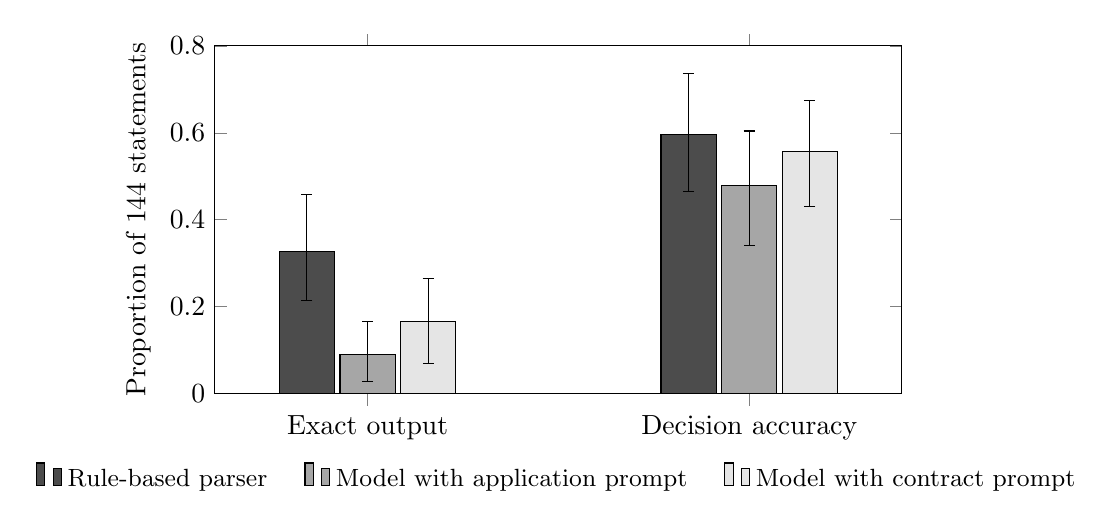
\begin{tikzpicture}
\begin{axis}[
  ybar, bar width=7mm, width=0.85\textwidth, height=6cm,
  ymin=0, ymax=0.8, ylabel={Proportion of 144 statements},
  symbolic x coords={Exact output, Decision accuracy}, xtick=data,
  enlarge x limits=0.4, legend style={at={(0.5,-0.18)}, anchor=north, legend columns=-1, draw=none, font=\small, /tikz/every even column/.append style={column sep=4mm}},
  error bars/y dir=both, error bars/y explicit]
\addplot[fill=black!70] coordinates {(Exact output,0.326) += (0,0.132) -= (0,0.111) (Decision accuracy,0.597) += (0,0.139) -= (0,0.132)};
\addplot[fill=black!35] coordinates {(Exact output,0.090) += (0,0.077) -= (0,0.062) (Decision accuracy,0.479) += (0,0.125) -= (0,0.139)};
\addplot[fill=black!10] coordinates {(Exact output,0.167) += (0,0.097) -= (0,0.098) (Decision accuracy,0.556) += (0,0.118) -= (0,0.125)};
\legend{Rule-based parser, Model with application prompt, Model with contract prompt}
\end{axis}
\end{tikzpicture}
\caption{Exact output and decision accuracy of the three interpretation methods on the development statements. Error bars are the 95\% intervals from Table~\ref{tab:llm}; those of the parser and of the model with the contract prompt overlap.}
\label{fig:llm}
\end{figure}

\paragraph{First run: application prompt.} Only 18 of the 144 outputs passed the contract check. The main reason was a mismatch between the application and the evaluation contract, not only the model. The application's prompt had been extended after the contract was fixed in October: it describes rule types such as preferred teaching windows and daily teaching limits, and a parameter field, which the contract does not know. The model used them in 56 proposals. The prompt also did not list the guide's clarification codes, so the model invented its own (for example \texttt{clarify\_if\_needed}), and clarification F1 was zero. Decisions are scored separately from the vocabulary, and they show a real behaviour: the model mostly answered \texttt{ready}. It treated 24 of 44 statements that need a question, all 8 conflicts and 11 of 16 unsupported requests as ready, and it referred to identifiers that were not in the context in 16 cases.

\paragraph{Second run: contract prompt.} With the contract's vocabulary and codes in the prompt, 122 outputs were valid and exact output nearly doubled, from 13 to 24. The model now asked more often: it recognised 25 of the 44 statements that need a question, against 5 in the first run, but it also asked in 16 of 76 clear statements. Exact outputs by language were 8 (English), 8 (formal Arabic), 3 (Egyptian Arabic) and 5 (mixed) of 36. Three errors remained:
\begin{itemize}
\item \emph{Wrong rule kind.} The model produced 161 weekly-limit proposals where the labels have 8. In 57 of them it represented a day-specific unavailability (``cannot teach Sunday 08:00--10:00'') as a weekly limit of zero hours, which the prompt's phrase ``0 forbids teaching'' probably invited; in 79 it added a 12-hour limit that the statement did not mention. This explains why recall rose to 0.41 while precision stayed at 0.17.
\item \emph{Conflicts.} None of the 8 conflicting statements was recognised; 5 of them produced no valid output.
\item \emph{Invalid replies.} The 12 invalid replies each took 330 to 383 seconds and contained no complete JSON, which suggests that the model reached the output limit while generating.
\end{itemize}

\paragraph{Comparison with the parser.} The parser remained higher on every measure except unsupported requests, where it scores zero by design (Section~\ref{evidence-baseline}). The intervals of the parser and of the second model run overlap for exact output and decision accuracy, so these 144 statements cannot show a reliable difference on those two measures; the parser's advantage in proposal and field F1 is clearer. Both methods were adjusted on the same development data, the parser after its first run and the model prompt by writing the code meanings from the labels, so neither figure is an estimate for unseen statements.

\paragraph{A label inconsistency.} Writing the code list for the second prompt showed that the draft labels use two codes for a missing day (\texttt{day\_required} and \texttt{missing\_day}) and two for minute-precise rules. A method cannot know which of two synonyms is expected, so a few clarification and unsupported errors of both methods are noise in the labels. The labels were not changed for these runs; the codes should be merged before the labels are reviewed.

\section{Automated check of the draft labels}\label{evidence-labelcheck}
The interpretation results above rely on draft labels that no human has reviewed (Section~\ref{dataset-construction}). A human audit of a stratified sample was prepared but not carried out. Instead, all 144 labels of the 0.2.1 bundle (guide~v2.1) were checked automatically on 28 November 2026. This is a consistency check, not a review: it was written and run by the same AI assistant that drafted the labels and the guide, so it shares their blind spots, and the labels keep the status ``draft, unreviewed''.

\paragraph{Mechanical checks.} A script checked every label for: a decision that matches its content (for example, \texttt{ready} with at least one proposal and no codes); clarification and unsupported codes that are current guide codes; instructor, room, group and activity IDs that exist in the context; days inside the context's week; whole hours inside the teaching day; hard strength for closures and soft strength for preferences; locks that point at the context draft; clock times in the English statement that match the proposal hours; one label shared by all four translations of a family; and the same codes for families with the same proposal pattern. Deliberately broken labels were used to confirm that each check fires. No label failed a check, and the four translations of every family carry the same label. One pattern check failed: \texttt{family-022} and \texttt{design-family-012} describe the same situation (a course whose only permitted window is fully covered by a closure of its group) but use different clarification codes, \texttt{hard\_window\_has\_no\_placement} and \texttt{resolve\_hard\_conflict}.

\paragraph{Reading against the guide.} The assistant also read each of the 36 families against the guide. It agreed with 33. The two families above disagree with each other; as with the synonyms merged in guide~v2.1 (Section~\ref{evidence-llm}), a method cannot know which code is expected, so one of the two should change. One family is ambiguous: \texttt{design-family-009} (``Studio~2 is closed on Saturday from 10:15 to 11:45'') is labelled unsupported because manual rules store whole hours, but unlike \texttt{family-020} it does not ask for exact times, and a 10:00--12:00 closure blocks exactly the same teaching period; the application's own outward rounding (Section~\ref{evidence-baseline}) would accept it. Three further notes concern wording only: two Arabic group names are paraphrases rather than context aliases, one formal Arabic statement says ``lectures'' where the others say ``classes'', and one statement lacks a day as well as a definition of ``early''. Together the three flagged families contain 12 of the 144 labels.

\paragraph{What it supports.} The check supports the statement that the draft labels are internally consistent, apart from one pair of families with different codes and one ambiguous family. It does not show that the labels are correct, and it is not independent or double annotation. No label was changed; a correction belongs in a new bundle version with a correction log.

\section{Reports and exports}
The statistics report for the published draft was recomputed independently from the saved assignments; every figure matched (448/448 sessions, sessions per day, zero overlaps, 65/65 rooms, 123/123 instructors, 22.97\% room time, no extra teaching hours). The review found that seat use ignored advising students, that unset limits were printed as ``None'', and that a report could not be limited to one group; all three were corrected. Timetable PDFs are now generated on the server as landscape A4 pages with short descriptive names (for example ``BA Y3 G7 Schedule'') because browser printing in one environment rotated the page and named the file after the application window.


\section{The JAI assistant: evaluation}\label{evidence-jai-results}

\paragraph{Automatic checks on held-out cases.} Each candidate answered the same held-out cases with the production prompt, at temperature~0. The automatic checks cover only whether the reply is valid, whether it wrongly proposes an action, whether it is in the user's language and whether it stays under 80 words; they do not judge correctness. Table~\ref{tab:jai-auto} reports the conversation cases with the guide in the prompt.

\begin{table}[h]
\centering
\small
\begin{tabular}{@{}lrrrrr@{}}
\toprule
16 held-out conversation cases & Base & v1 & v2 & v3 & v4 \\
\midrule
Valid reply & 16 & 16 & 16 & 16 & 16 \\
No wrongly proposed action & 15 & 16 & 15 & 16 & 16 \\
Reply in the user's language & 16 & 13 & 12 & 14 & 14 \\
At most 80 words & 14 & 16 & 12 & 14 & 16 \\
\midrule
Action choice (5 separate cases) & 3 & 5 & 5 & 4 & 5 \\
\bottomrule
\end{tabular}
\caption{Automatic checks. Base, v1 and v2 were run on 22 November; v3 on 23 November with the extended guide, where v1 re-run on identical prompts gave 13 replies in the user's language and 16 under 80 words; v4 on 24 November with the same prompts as v3.}
\label{tab:jai-auto}
\end{table}

Round~2 is a negative result worth recording. Its training answers had been written before the guide existed and were left unchanged when the guide was added to the prompts, so the model was trained to receive the guide and then answer in its own words; it invented more than v1 (``snapshots on the cloud'', solver settings that do not exist). Lower training loss with an extra epoch reflected memorisation of 210 rows rather than better answers. Round~3 rewrote the answers so that every statement about JadwAI comes from the guide entries present in that example's prompt, and the dataset builder now refuses an example whose prompt lacks the guide entries its answer relies on.

\paragraph{Blind human rating.} For v1 and v3, the 19 held-out conversation answers (16 cases and three wordings of a new ``not sure'' question) were placed side by side in random order, without model names, and scored from 1 to 5 on correctness, logic, helpfulness and natural language (Table~\ref{tab:jai-rating}). The rater was the project owner, who had read a short summary of some replies beforehand, so the rating is neither independent nor fully blind.

\begin{table}[h]
\centering
\small
\begin{tabular}{@{}lrr@{}}
\toprule
19 cases, 4 criteria, 1--5 each & v1 & v3 \\
\midrule
Total (maximum 380) & 244 & 274 \\
Mean per case (maximum 20) & 12.8 & 14.4 \\
Correct / logical / helpful / natural (means) & 3.3 / 3.3 / 3.1 / 3.2 & 3.7 / 3.6 / 3.6 / 3.5 \\
Cases won (8 ties) & 3 & 8 \\
\bottomrule
\end{tabular}
\caption{Blind side-by-side rating of fine-tuned v1 and v3.}
\label{tab:jai-rating}
\end{table}

The largest gains were in Arabic: an Arabic privacy question that v1 answered in English, and a request for ``no classes at 08:30'' that v1 answered by claiming such classes were forbidden, while v3 correctly said no mandatory rule prevents them. Six cases received the minimum score for both models, including an off-topic request for a poem and an Arabic question about shared lectures.

\paragraph{Live use.} With v3 in the running application, four questions taken from the weakest cases were asked in the chat. The display of mixed Arabic and English text was correct after the fix described in Section~\ref{evidence-jai}, but the answers were weak: an Arabic question about laboratories with GPUs used wrong words for rooms; the poem request produced a poem; a frustrated Arabic message drifted into Chinese mid-sentence; and a question about connecting to the university's student information system, asked after the complaint, was answered with a request for a rule identifier from the previous topic. The held-out measurements therefore overstate live reliability, particularly for topic changes within one conversation. These cases were used to write a fourth round of training examples (off-topic requests, topic changes, Arabic room vocabulary and examination publishing), which were trained as round~4 (v4; Table~\ref{tab:jai-rounds}).

\paragraph{Round 4.} On the old held-out cases v4 matched v3 on validity, actions and language, kept every reply under 80 words and chose the examination timetable correctly in the action case that v3 had missed (Table~\ref{tab:jai-auto}); it was also about 12\% faster per answer. Round~4 also held out one new family for each live failure, 13 cases in total, which neither model had seen (Table~\ref{tab:jai-round4}).

\begin{table}[h]
\centering
\small
\begin{tabular}{@{}lrr@{}}
\toprule
13 new held-out cases (4 families) & v3 & v4 \\
\midrule
Right action (none, or the expected one) & 10 & 9 \\
Reply in the user's language & 9 & 10 \\
At most 80 words & 12 & 13 \\
Mentions an internal API path & 1 & 2 \\
\bottomrule
\end{tabular}
\caption{Round-4 held-out families: off-topic story (3), changing topic from a rule to the portal (3), adding a laboratory with GPUs (4) and a formal request to publish the examination timetable (3).}
\label{tab:jai-round4}
\end{table}

These automatic differences are within one or two cases and do not by themselves show that v4 is better. Reading the replies shows where it changed. Both models declined the English story requests; in Arabic, v3 drifted into a long, repetitive timetable summary, while v4 stayed short but mixed in an English phrase. For the English GPU questions v4 gave the right steps (add a room with the laboratory type and the GPU feature), where v3 asked which room was being replaced. Neither model answered the Arabic GPU questions in Arabic, and v4 quoted an internal API path in both of them. Neither model turned ``publish the exam schedule'' in conversation into the publish action in any of the three cases, so the examination examples in round~4 did not fix the failure they targeted. The project owner then rated v3 and v4 side by side on all 32 cases (the 19 earlier cases and the 13 new ones) in the same way as before, again after reading a summary of the automatic results and some replies (Table~\ref{tab:jai-rating-v4}).

\begin{table}[h]
\centering
\small
\begin{tabular}{@{}lrr@{}}
\toprule
32 cases, 4 criteria, 1--5 each & v3 & v4 \\
\midrule
Total (maximum 640) & 461 & 524 \\
Mean per case (maximum 20) & 14.4 & 16.4 \\
Correct / logical / helpful / natural (means) & 3.5 / 3.6 / 3.6 / 3.7 & 4.0 / 4.1 / 4.1 / 4.2 \\
Earlier 19 cases / new 13 cases (totals) & 293 / 168 & 317 / 207 \\
Cases won (12 ties) & 6 & 14 \\
\bottomrule
\end{tabular}
\caption{Blind side-by-side rating of fine-tuned v3 and v4. Scores from different sheets are not comparable: v3 received 293 here and 274 on the same 19 cases in Table~\ref{tab:jai-rating}.}
\label{tab:jai-rating-v4}
\end{table}

The rating favoured v4 on both the earlier and the new cases, unlike the automatic checks. The largest differences were an off-topic request for a poem (4 against 20 points), which v3 did not decline, the Arabic story request (8 against 20) and the Arabic portal question (10 against 20). v4 lost most clearly on an Arabic question about special rooms (14 against 10) and on one Arabic GPU question (10 against 4), where it quoted an internal interface path. Four cases received the minimum score for both models, among them a formal Arabic request to publish the examination timetable.

\paragraph{Examination publishing fixed in code.} Because four training rounds did not teach the model to turn ``publish the exam schedule'' into the publish action, this request is now recognised by a built-in pattern before the model is called, in English, formal Arabic and Egyptian Arabic. It prepares the publish action for the examination timetable on screen or named in the message and asks the administrator to confirm; when an examination and a teaching draft, or several examination drafts, could be meant, it asks which one instead of choosing. Twenty-five tests cover the wordings of the held-out family and the ambiguous cases. This is a change to the system, not to the model, so it does not alter the measurements above.


\paragraph{Live use with v4.} The four live questions were asked again on 24 November, of v4 in the running application, in the same order and in one chat (evidence folder \texttt{2026-11-24-live-v4}). The poem request was now declined with an offer of help with the examination timetable, and the frustrated Arabic message no longer drifted into Chinese. The Arabic question about laboratories with GPUs used the right words and stated the correct rule (a room needs every required feature, enough seats and a suitable type), but then repeated a sentence about room availability. Topic changes remained weak: the reply to the frustrated message continued the examination topic of the previous turn without acknowledging the user, and the question about the student information system was answered with a request for ``the CSV contents in the request body''. This points towards CSV import, which is the correct route, but in internal terms and without saying that a direct connection does not exist. Answers took between 3.5 and 10 minutes. A request to publish the examination timetable, added as a fifth message, was answered by the built-in route in 2 seconds with a question about which of the unpublished examination drafts to publish. Live use therefore confirms the gains seen in the rating for off-topic requests and Arabic vocabulary, and the remaining weakness in multi-turn topic changes.

\paragraph{Limits.} The examples and contexts are fictional and were drafted with AI assistance; approvals were bulk approvals by the project owner. The held-out sets are small (16--19 conversation cases, 13 round-4 cases and 5 action cases), the automatic checks do not measure correctness, and the human ratings had one rater who was not independent of the project and had seen summaries of the replies. All runs used one machine, one random seed and temperature~0. These results describe the development of a local assistant; they are not estimates of constraint-extraction accuracy (RQ1).

\section{A supervisor-style test}\label{evidence-supervisor}
On 28 November 2026 the demonstration workspace (780 weekly sessions, 174 groups, 65 rooms, 102 courses) was used as a timetabling supervisor would use it: a teaching timetable for the whole university, the first quiz round, the midterms and the finals, partly through the forms and partly through JAI. Each result was also checked by a separate script for overlaps, seats and dates.

\begin{itemize}
\tightlist
\item \textbf{Teaching timetable.} All 780 sessions were placed in three automatic parts of about four minutes each and passed validation. The days were uneven, however: 195 sessions on Saturday against 95 on Thursday. A term for the busiest day on campus was therefore added to the objective and to the independent recount. Regenerated, the days carried 127 to 131 sessions each; empty periods between classes fell from 36 to 20 and long days from 270 to 0 minutes, at the cost of 9 more group-days on campus across 174 groups.
\item \textbf{Quiz~1.} 102 quizzes of 30 minutes over six days were placed in seconds with no hall or invigilator clash.
\item \textbf{Midterms through JAI.} The request ``make the midterm schedule from 17 to 29 October, max 2 exams per day for each program'' produced 102 two-hour midterms inside the period, with no Friday, no clash and enough seats for every exam.
\item \textbf{Finals.} 102 three-hour finals and 102 second-chance midterms were placed in 18 days. In 53 courses the second chance came after the final, and 13 exams fell on 7 January, a public holiday in Egypt. A rule placing each second chance before its final and a list of dates to skip were added; regenerated with 7 January skipped, no exam was on that day and no second chance followed its final.
\end{itemize}

The test found eleven faults, all corrected with regression tests. Five were in the exam page and its exports (a page that scrolled sideways, drafts that could not be told apart, a summary that gave every exam two hours, a file name and an empty programme column). One was a garbled sentence on the teaching page, and five were in JAI: it read ``for each program'' as a programme name, ignored ``including second-chance midterms'', missed Egyptian Arabic date ranges such as ``17 to 29 October'' written with the short preposition \emph{li-}, chose next year for dates that had just passed, and answered ``how many exams can a program have per day?'' with a list of programmes. Repeated sign-ins by the checking script were blocked by the login rate limit, as designed.

\section{Automated tests and limitations of this evidence}
On 28 November 2026 the automated suites pass: 571 backend tests, 109 frontend tests and 50 evaluation-harness tests. They include regression tests for every fault reported in this chapter.

The evidence has the following limits. All measurements come from one machine and one random seed; repeated runs and other hardware may differ, and parallel search can produce different valid timetables from identical inputs. The university-scale run used adjusted data, so it demonstrates the mechanism rather than a timetable for the university. The demonstration workspace is derived from real course structures but uses invented names and advising students. The repair diagnosis returns a minimal rather than a minimum set of changes, depends on time budgets, and on large timetables searches locally first. The comparison with the real timetable uses placeholder rooms and staff and copied days off (Section~\ref{evidence-real}). The interpretation results use draft labels reviewed by no human (checked automatically only, Section~\ref{evidence-labelcheck}), a single development release, a parser and a model prompt prepared by the same author who wrote the corpus, and one run of the model. A confirmatory answer to RQ1 and RQ2 would require reviewed labels and a fresh held-out set, and RQ3 would require the participant study outlined in Section~\ref{meth-rq3}.


\chapter{Conclusion and Future Work}\label{chap:conclusion}

% NOTE (24 Nov 2026): First draft written from the Results chapter at the owner's request (drafted with AI assistance; reword in your own words before submission). Every figure is taken from Chapter~\ref{evidence}; update this chapter if those figures change (for example after the v3/v4 blind rating).

This thesis set out to let university administrators state timetabling requirements in their own words, in English or Arabic, and to have those requirements turned into formal rules that a solver can use, without letting a wrong interpretation reach a published timetable. This chapter answers the research questions from the evidence in Chapter~\ref{evidence}, states what the work contributes, and lists its limits and the work that would follow.

\section{Answers to the research questions}

\paragraph{RQ1: extraction accuracy.} On the 144 development statements, the rule-based parser produced the exact expected output for 32.6\% of them (95\% interval 21.5--45.8\%). The local language model reached 9.0\% with the application's prompt and 16.7\% (6.9--26.4\%) with a prompt written for the evaluation contract. The parser was also ahead on proposal and field agreement. The intervals overlap for exact output and decision accuracy, so these data do not show a reliable difference on those two measures. Most of the model's errors were systematic rather than random: it represented a day-specific unavailability as a weekly limit of zero hours and added weekly limits that no statement mentioned. Both methods did worse on Egyptian Arabic than on English. The answer to RQ1 is therefore limited: a seven-billion-parameter model running on a laptop, constrained to the contract's schema, did not extract rules more accurately than a hand-written parser on this corpus. Because the labels are draft, the statements are synthetic and both methods were adjusted on the same data, this is development evidence and not an estimate for real administrators' statements.

\paragraph{RQ2: asking instead of guessing.} The parser recognised missing or ambiguous information with a clarification F1 of 0.351. The model with the application's prompt treated most incomplete statements as ready (24 of 44) and never used the guide's codes. With the codes in its prompt, it recognised 25 of the 44 statements that needed a question, but it also asked in 16 of 76 clear statements, and it recognised none of the 8 conflicting ones. Neither method handled unsupported requests well. The answer to RQ2 is that the model can be moved from guessing towards asking by the prompt, but not yet to asking at the right time. In the system as built this matters less than the figures suggest, because every interpretation is shown to the administrator and nothing reaches the solver without approval.

\paragraph{RQ3: AI-assisted versus manual entry.} This question could not be answered. No participants or ethics approval were available during the project, so no entry times or correction counts were measured. The study design remains in Section~\ref{meth-rq3}.

\paragraph{RQ4: base versus fine-tuned local model.} Fine-tuning changed the assistant's behaviour, but not always for the better. The first round improved the choice of actions (5 of 5 against 3 of 5 for the base model) but replied in the user's language less often; the second, which added the guide to the prompts without rewriting the answers, made the model invent more and was discarded; the third, whose answers were rewritten to use only the guide's facts, was preferred in the blind rating (274 against 244 of 380 points for round~1). The fourth round kept every reply under 80 words, fixed the action choice for examination timetables and was preferred over round~3 in a second blind rating (524 against 461 of 640 points), although the automatic checks on 13 new held-out cases differed by only one or two cases. Neither model turned a conversational request to publish the examination timetable into the publish action, so that request is now handled by a built-in pattern. In live use, v4 declined an off-topic request and kept to Egyptian Arabic where v3 had not, but it still lost track when the topic changed within one conversation. Latency stayed at five to six minutes per answer on the test laptop, at no cost per call. The answer to RQ4 is that fine-tuning on reviewed, guide-grounded examples improved a local model in small, measurable steps, that the content of the training answers mattered more than the number of epochs, and that some failures were not fixed by more examples.

\paragraph{Supporting engineering question.} The validator and the approval workflow did what they were built to do. Every timetable reported as valid was checked by an independent validator that does not use the solver's model, only approved rules reached the solver, and publication re-validated the timetable first. The department-scale timetable (448 sessions) and the university-scale timetable built in six parts (2{,}703 sessions on adjusted data) both passed validation, and impossible inputs were explained by a minimal set of changes that was itself verified. This is the main reason the modest extraction results do not make the system unsafe: a wrong interpretation can waste an administrator's time, but it cannot silently enter a published timetable.

\section{Contributions}

The work contributes, in proportion to the evidence:
\begin{itemize}
\item a closed set of supported timetabling rules and a machine-readable output contract with explicit decisions for clarification, unsupported and conflicting requests;
\item a synthetic development corpus of 144 statements in English, formal Arabic, Egyptian Arabic and mixed language, with a versioned annotation guide and an offline scorer that reports intervals over intent families;
\item a development-level comparison of a rule-based parser and a local language model with two prompts, including the finding that a mismatch between an application's prompt and its evaluation contract can dominate the measured result;
\item a four-round fine-tuning study of a local assistant model, including a round that made the model worse and the reason for it, and a method for merging adapters into quantised weights without losing the training;
\item a working prototype for teaching and examination timetables in which approval and independent validation keep unreviewed or invalid output from being used.
\end{itemize}
No claim is made about accuracy on real administrators' statements or about reduced administrative effort.

\section{Limitations}

The interpretation labels were drafted by the author with AI assistance and have not been reviewed by an independent annotator; two pairs of codes in them turned out to be synonyms, which were merged in guide~v2.1 after the runs reported here. The corpus is small and synthetic, and both the parser and the model prompt were adjusted after looking at the same development data, so their figures are optimistic. All model runs used one laptop, one seed and temperature~0, and the model was run once per prompt. No commercial model was compared, because no budget for paid calls was approved. The fine-tuning examples and contexts are fictional, approvals were bulk approvals by the project owner, the held-out sets contain 5 to 19 cases per measure, and both blind ratings had one rater who was not independent of the project. The university-scale timetable used adjusted data with placeholder staff and rooms. Finally, RQ3 has no evidence at all.

\section{Future work}

\begin{itemize}
\item \textbf{Reviewed labels and a held-out set.} Two independent annotators should review the development labels of guide~v2.1, in which the duplicate codes are merged, agreement should be measured, and a fresh set of statements should be written and kept unseen until a final run. This is the step that would turn the RQ1 and RQ2 results into confirmatory evidence.
\item \textbf{The participant study (RQ3).} A small study with timetabling staff, comparing form entry with AI-assisted entry on the same requirements, would measure time, corrections and interpretation errors.
\item \textbf{Better extraction.} The model's systematic errors suggest specific changes: describing weekly limits more narrowly in the prompt, giving examples of conflicts, and fine-tuning the extraction task in the same way as the assistant. A larger local model or a commercial model, if a budget is available, would show how much of the gap is due to model size.
\item \textbf{The assistant.} Publishing the examination timetable was moved to a built-in pattern after training did not fix it; other requests that training does not fix can be handled the same way. Arabic replies about rooms and laboratories, and replies that mention internal interface paths, need further examples or output checks. Faster hardware would make the assistant usable in daily work.
\item \textbf{Scheduling.} Optimising earlier parts of a university-scale timetable after later parts are placed, and testing with the university's real staff and room data, would show whether the part mechanism is sufficient in practice.
\end{itemize}

The overall conclusion is that a local language model can help administrators state timetabling requirements in their own language, but on the evidence of this project it should do so as a proposer whose output is checked, approved and validated, not as an interpreter whose output is trusted.

\appendix
\renewcommand{\appendixtocname}{Appendix}
\renewcommand{\appendixpagename}{\appendixtocname}
\addappheadtotoc
\setboolean{@twoside}{false}
\appendixpage

\chapter{Lists}
\addcontentsline{toc}{section}{List of Abbreviations}
\begin{acronym}[\hspace{3cm}]
  \acro{API}{Application Programming Interface}
  \acro{CP-SAT}{Constraint Programming / Boolean Satisfiability solver (Google OR-Tools)}
  \acro{CSV}{Comma-Separated Values}
  \acro{JAI}{The JadwAI assistant}
  \acro{LLM}{Large Language Model}
  \acro{LoRA}{Low-Rank Adaptation}
  \acro{NFR}{Non-Functional Requirement}
  \acro{FR}{Functional Requirement}
  \acro{QLoRA}{Quantised Low-Rank Adaptation}
  \acro{RQ}{Research Question}
  \acro{SRS}{Software Requirements Specification}
  \acro{TA}{Teaching Assistant}
\end{acronym}
\clearpage
\listoffigures
\addcontentsline{toc}{section}{List of Figures}
\listoftables
\addcontentsline{toc}{section}{List of Tables}

\chapter{Functional and Non-Functional Requirements}\label{app:requirements}

The complete list of requirements, with a one-sentence summary and the prototype status of each, is kept with the source code:

\begin{center}
\url{https://github.com/rawdatarekkkk/jadwai/blob/main/docs/REQUIREMENTS.md}
\end{center}

It is derived from the project's Software Requirements Specification (SRS) v0.4 of 18 November 2026, which defines the inputs, outputs, error behaviour and acceptance criteria of every requirement. SRS v0.2 was reviewed by the supervisor; v0.3 and v0.4 carry the project owner's approval only. The status is the owner's record of the prototype on 23 November 2026, not a supervisor acceptance or a research result: \emph{implemented} means working in the prototype with automated tests, \emph{partial} that a working subset exists.

\section{Functional requirements}

Table~\ref{tab:fr-areas} groups the 78 functional requirements by area. Of these, 55 are implemented, 17 partly implemented and 6 not started.

\begin{longtable}{@{}p{0.26\textwidth}p{0.17\textwidth}p{0.155\textwidth}p{0.33\textwidth}@{}}
\caption{Functional requirements by area.}\label{tab:fr-areas}\\
\toprule
Area & Requirements & Status & Main gaps \\
\midrule
\endfirsthead
\toprule
Area & Requirements & Status & Main gaps \\
\midrule
\endhead
Term data and records & FR-001--FR-008 & Partial & One term only; no aliases or dated availability exceptions \\
Constraint vocabulary and lifecycle & FR-009--FR-013 & Partial & No supersession history or weight editing \\
AI extraction and review & FR-014--FR-023, FR-073, FR-074 & Partial & Extraction measured on development data only (Section~\ref{evidence-llm}); no audit export with cost \\
Scheduling & FR-024--FR-030, FR-065--FR-070 & Implemented & --- \\
Validation & FR-031--FR-033 & Implemented & --- \\
Scenarios and editing & FR-034--FR-039 & Partial & No explicit-variation scenarios (FR-037) \\
Publication and views & FR-040--FR-043, FR-078 & Implemented & --- \\
Export & FR-044, FR-045 & Implemented & --- \\
Traceability, accounts, audit & FR-046--FR-048 & Partial & Partial requirement-to-publication trace \\
Evaluation support & FR-049, FR-050 & Partial & No human annotations; no participant study \\
Examinations & FR-051, FR-071, FR-072 & Implemented & --- \\
Ask JAI & FR-075--FR-077 & Implemented & --- \\
Infeasibility explanation & FR-058 & Implemented & --- \\
Extensions & FR-052--FR-057 & Mostly not started & Arabic extraction (FR-054) works but is unmeasured \\
Exception handling & FR-059--FR-064 & Partial & Cancelled results are not retained \\
\bottomrule
\end{longtable}

\section{Non-functional requirements}

The SRS defines 23 non-functional requirements and invents no numeric targets; values that depend on later decisions remain open. Table~\ref{tab:nfr} summarises them.

\begin{longtable}{@{}p{0.19\textwidth}p{0.17\textwidth}p{0.56\textwidth}@{}}
\caption{Non-functional requirements and prototype status.}\label{tab:nfr}\\
\toprule
Category & Requirements & Status \\
\midrule
\endfirsthead
\toprule
Category & Requirements & Status \\
\midrule
\endhead
Correctness & NFR-001--003 & Met in tests: separate validator; publication refused on any violation; a time limit is never reported as infeasibility \\
Security & NFR-004, 005 & Server-side permissions; no secrets in the repository. Passwords use scrypt instead of the specified Argon2id (recorded deviation) \\
Privacy & NFR-006, 007 & With the local model no text leaves the server; applicable data-protection rules still to be confirmed \\
Accessibility & NFR-008 & Labelled, keyboard-operable controls; no formal audit \\
Reliability & NFR-009, 010 & Timeouts, retries, malformed output and cancellation tested; recovery objectives open \\
Performance and scale & NFR-011--013 & Runtime, outcome and tested scale recorded with every result; no numeric targets \\
Usability & NFR-014, 015 & Checked manually; not measured (no participant study) \\
Reproducibility & NFR-016 & Versions, seeds and dates recorded for runs and fine-tuning \\
Maintainability & NFR-017 & Separate modules; model provider chosen by configuration \\
Compatibility, retention, backup & NFR-018--020 & Open; local backups before destructive changes \\
Localisation & NFR-021 & English and Arabic interface with right-to-left layout; mixed Arabic/English text kept in reading order \\
Observability, licensing & NFR-022, 023 & Partial; licence list not yet checked \\
\bottomrule
\end{longtable}

\chapter{Screenshots of the Prototype}\label{app:screenshots}

The following screenshots were taken from the running prototype on 23 November 2026 in the demonstration workspace (a browser window of 1440$\times$900 pixels). All names of people are demonstration placeholders. Further screenshots are in the repository folder \texttt{docs/screenshots}.

\begin{figure}[p]
\centering
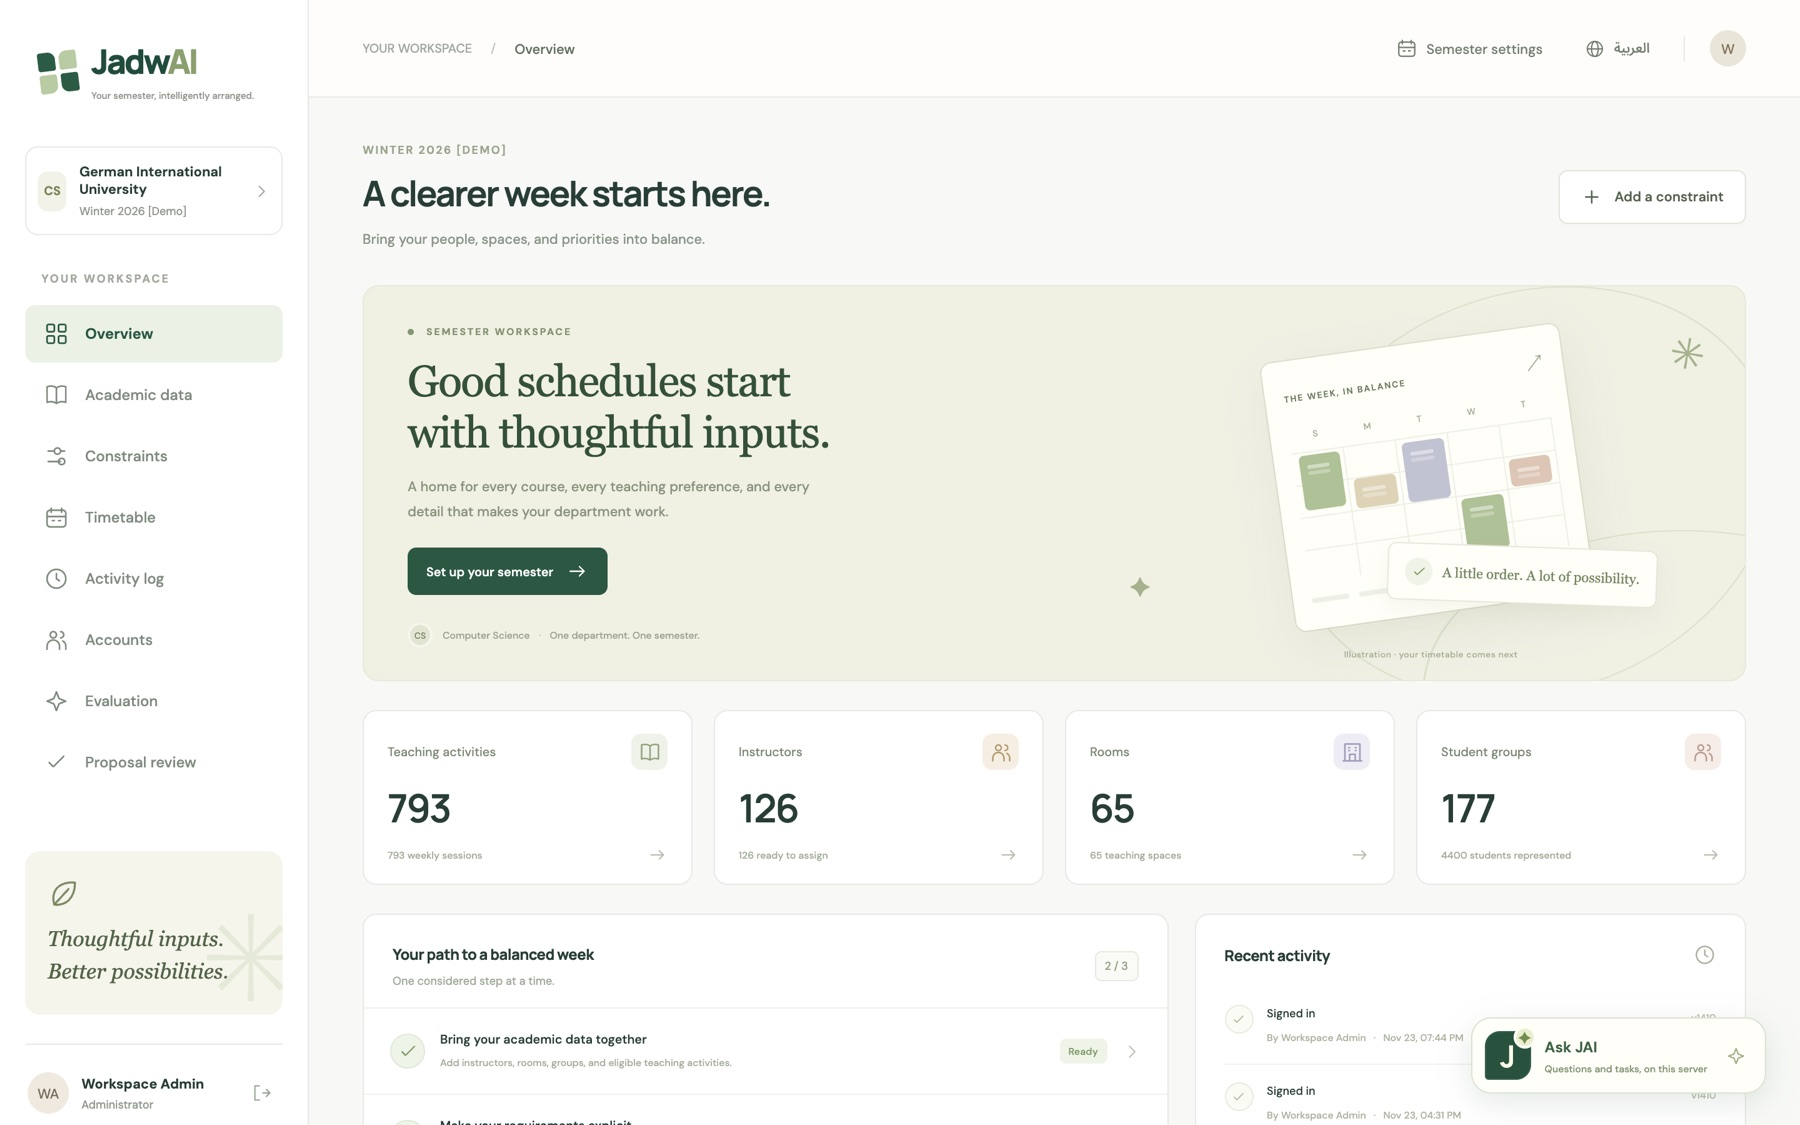
\includegraphics[width=\textwidth]{02-overview.jpg}
\caption{Overview page of the administrator workspace: counts of activities, instructors, rooms and student groups, the setup path and recent activity.}
\label{fig:shot-overview}
\end{figure}

\begin{figure}[p]
\centering
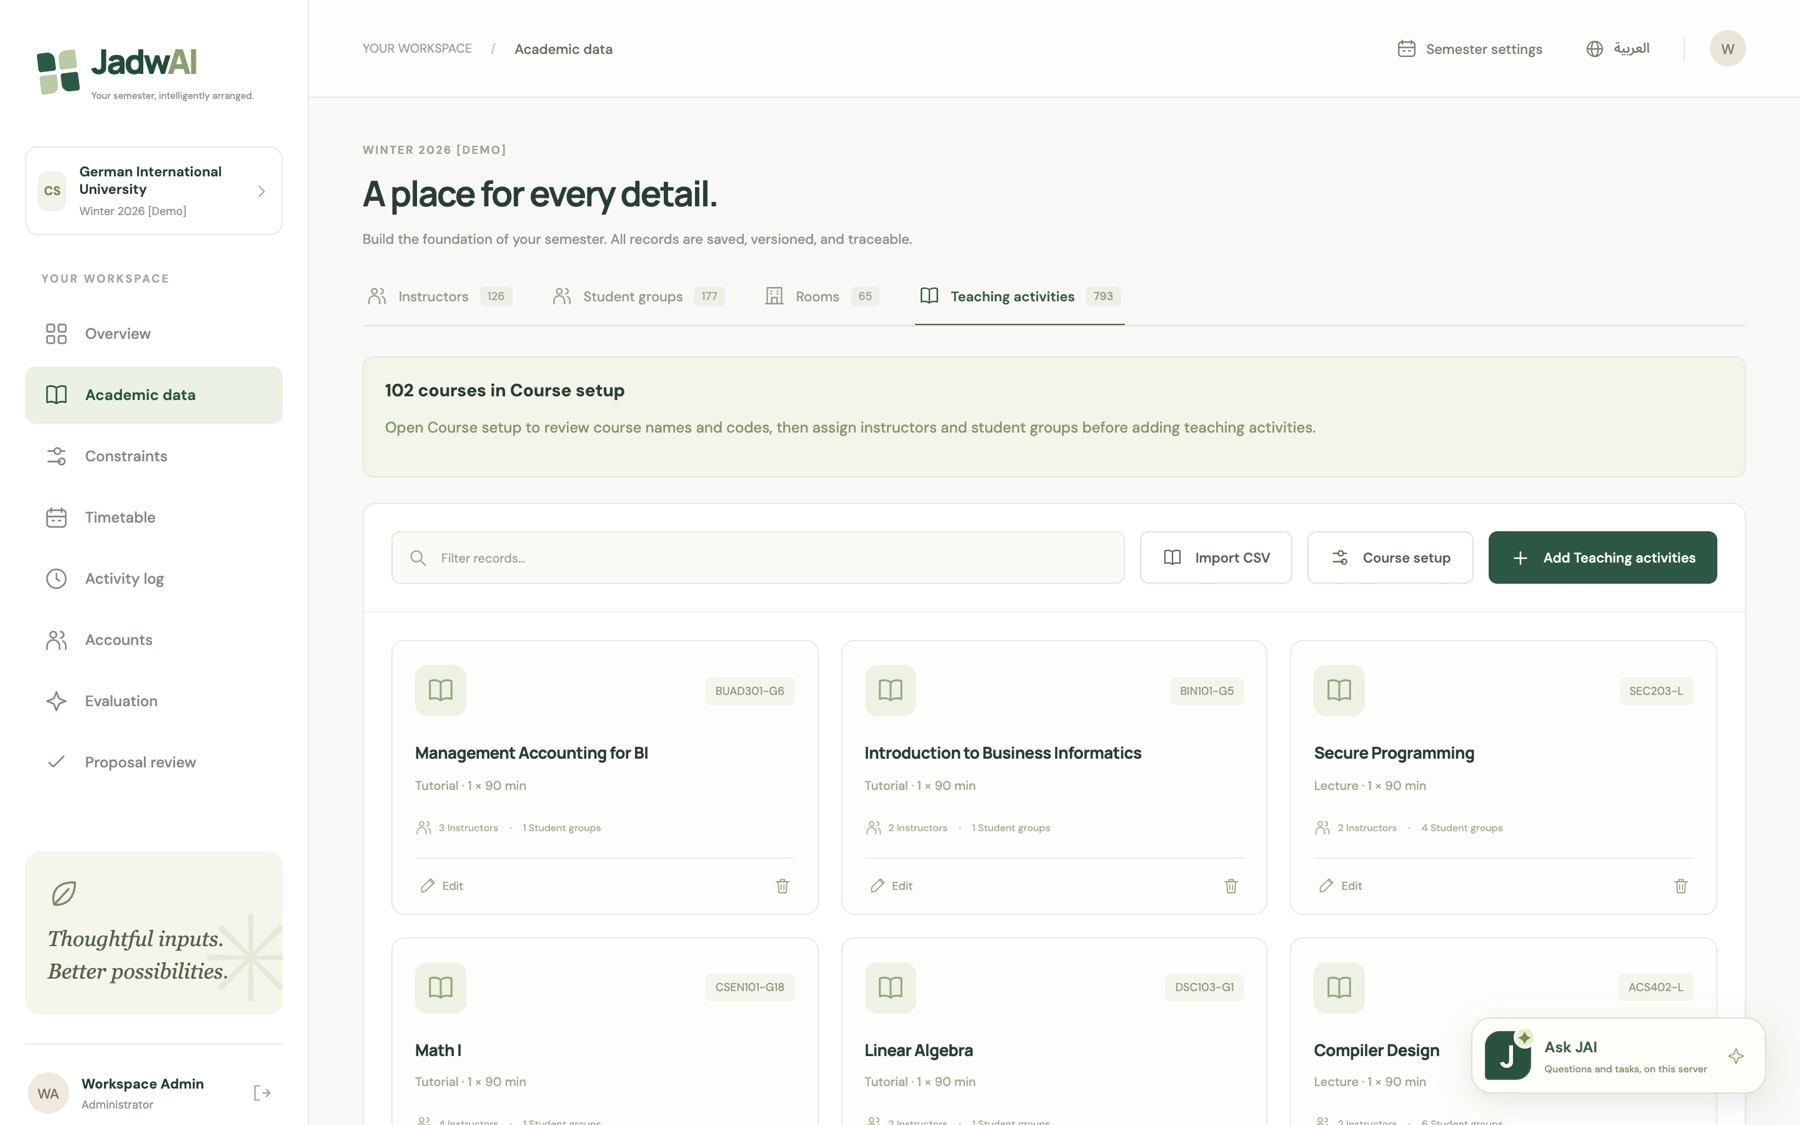
\includegraphics[width=\textwidth]{03-academic-data.jpg}
\caption{Academic data: teaching activities of each course, with separate tabs for instructors, student groups and rooms, and CSV import.}
\label{fig:shot-academic-data}
\end{figure}

\begin{figure}[p]
\centering
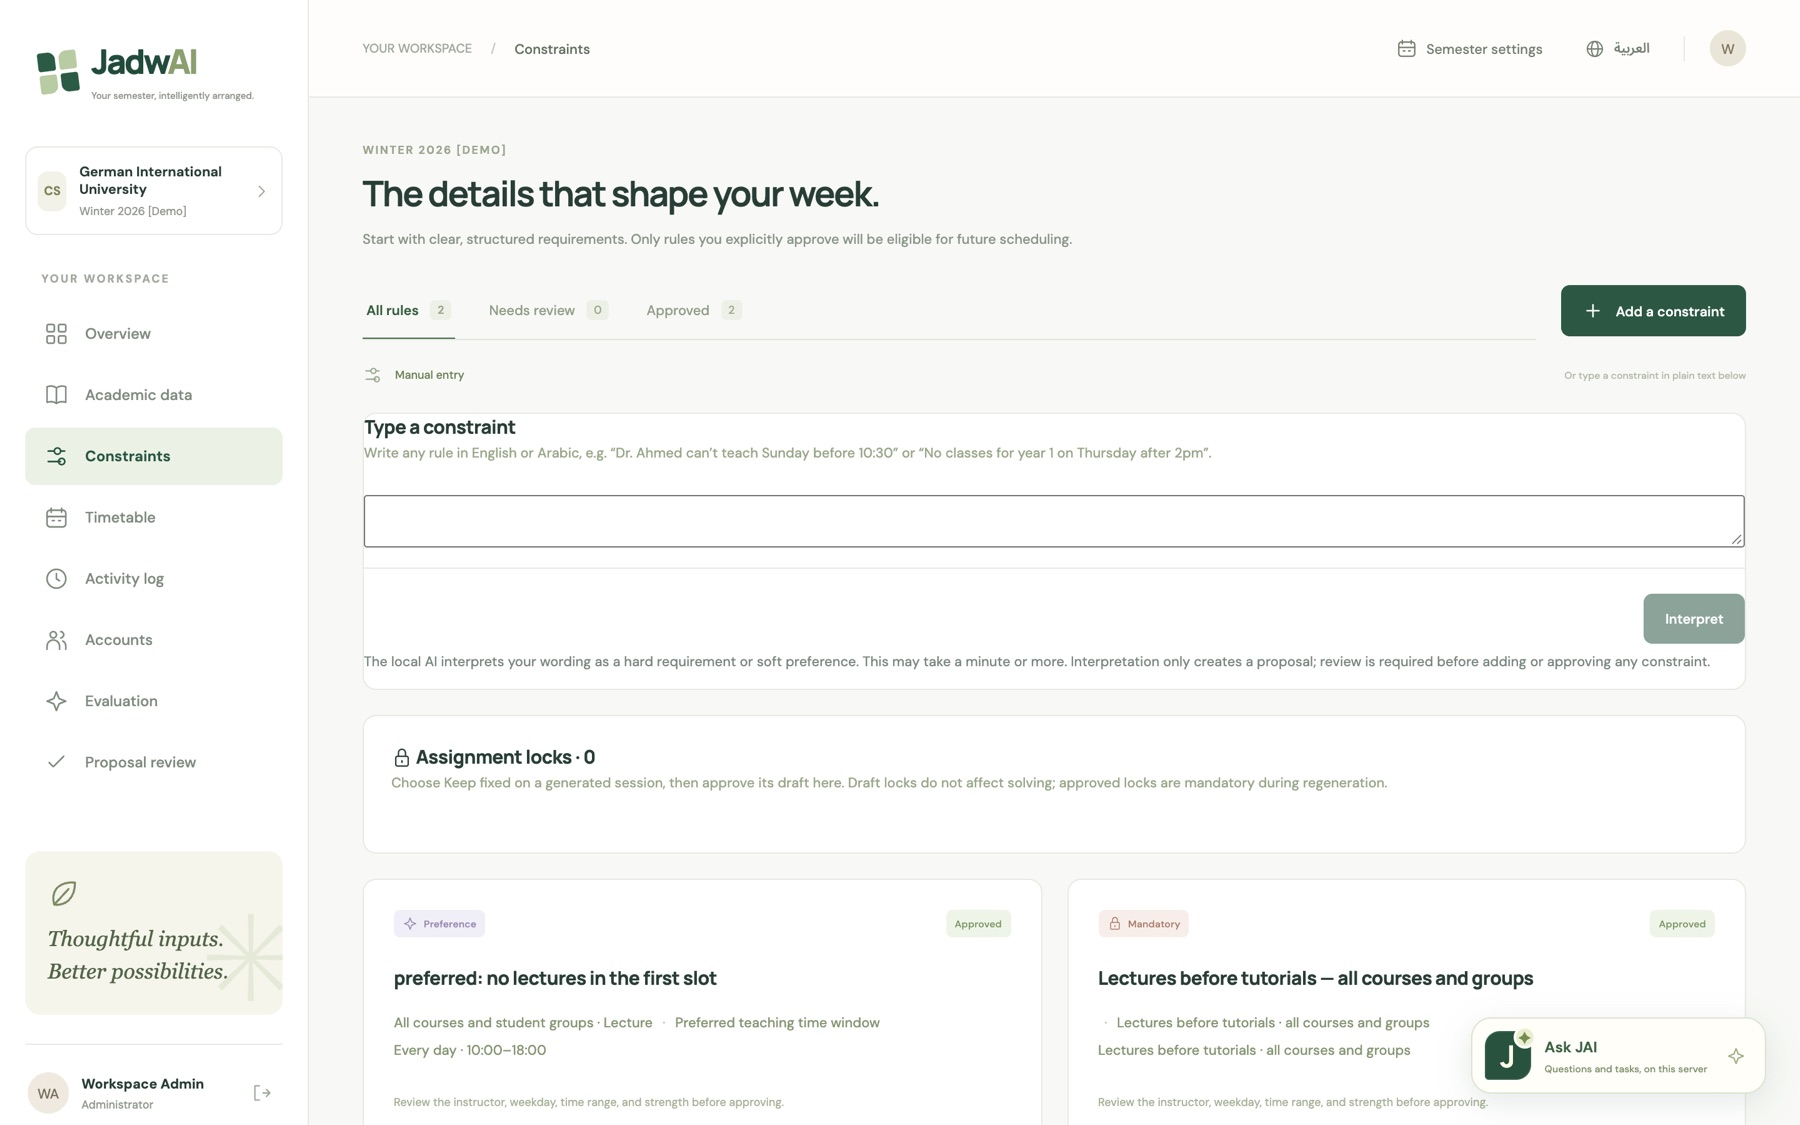
\includegraphics[width=\textwidth]{04-constraints.jpg}
\caption{Constraints: a requirement can be typed in English or Arabic and is interpreted as a proposal; approved rules are listed below with their strength (preference or mandatory).}
\label{fig:shot-constraints}
\end{figure}

\begin{figure}[p]
\centering
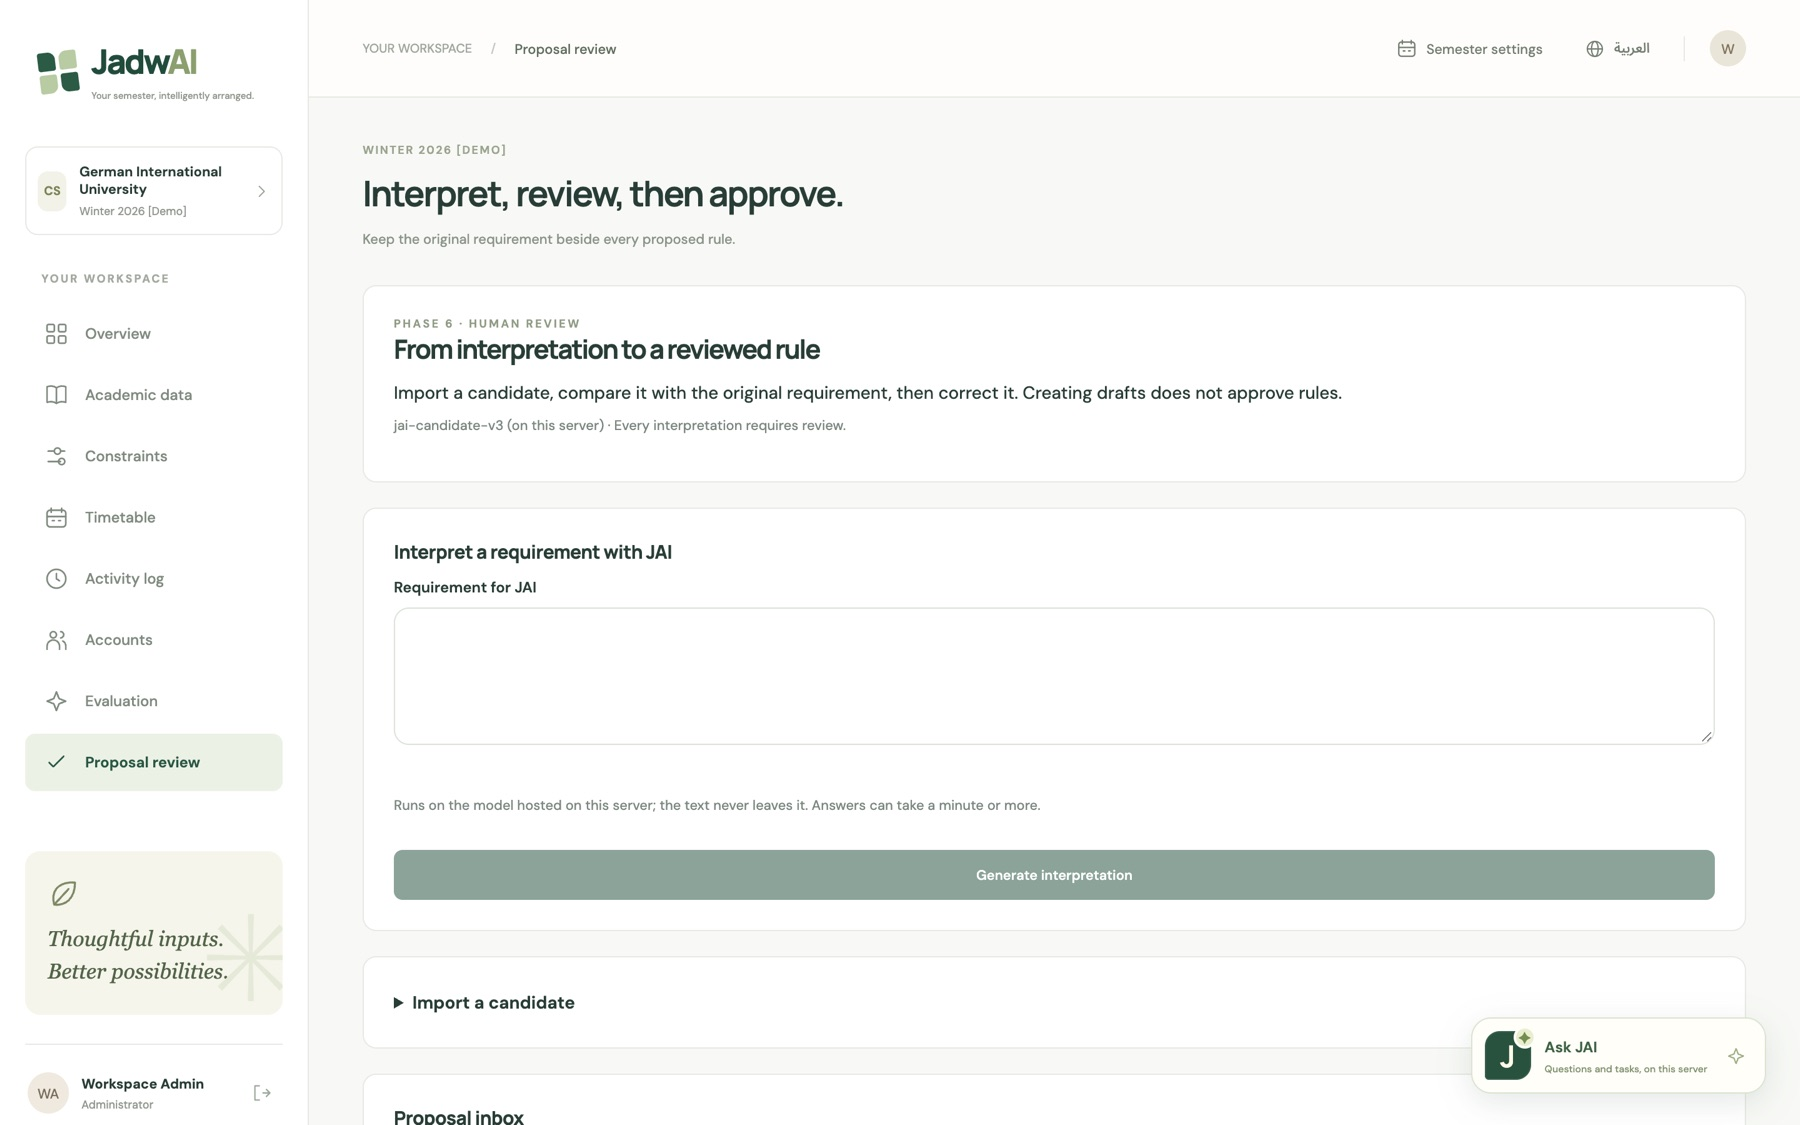
\includegraphics[width=\textwidth]{09-proposal-review.jpg}
\caption{Proposal review: a requirement is interpreted by the locally hosted model and shown beside the original text for correction before any rule is created.}
\label{fig:shot-proposal-review}
\end{figure}

\begin{figure}[p]
\centering
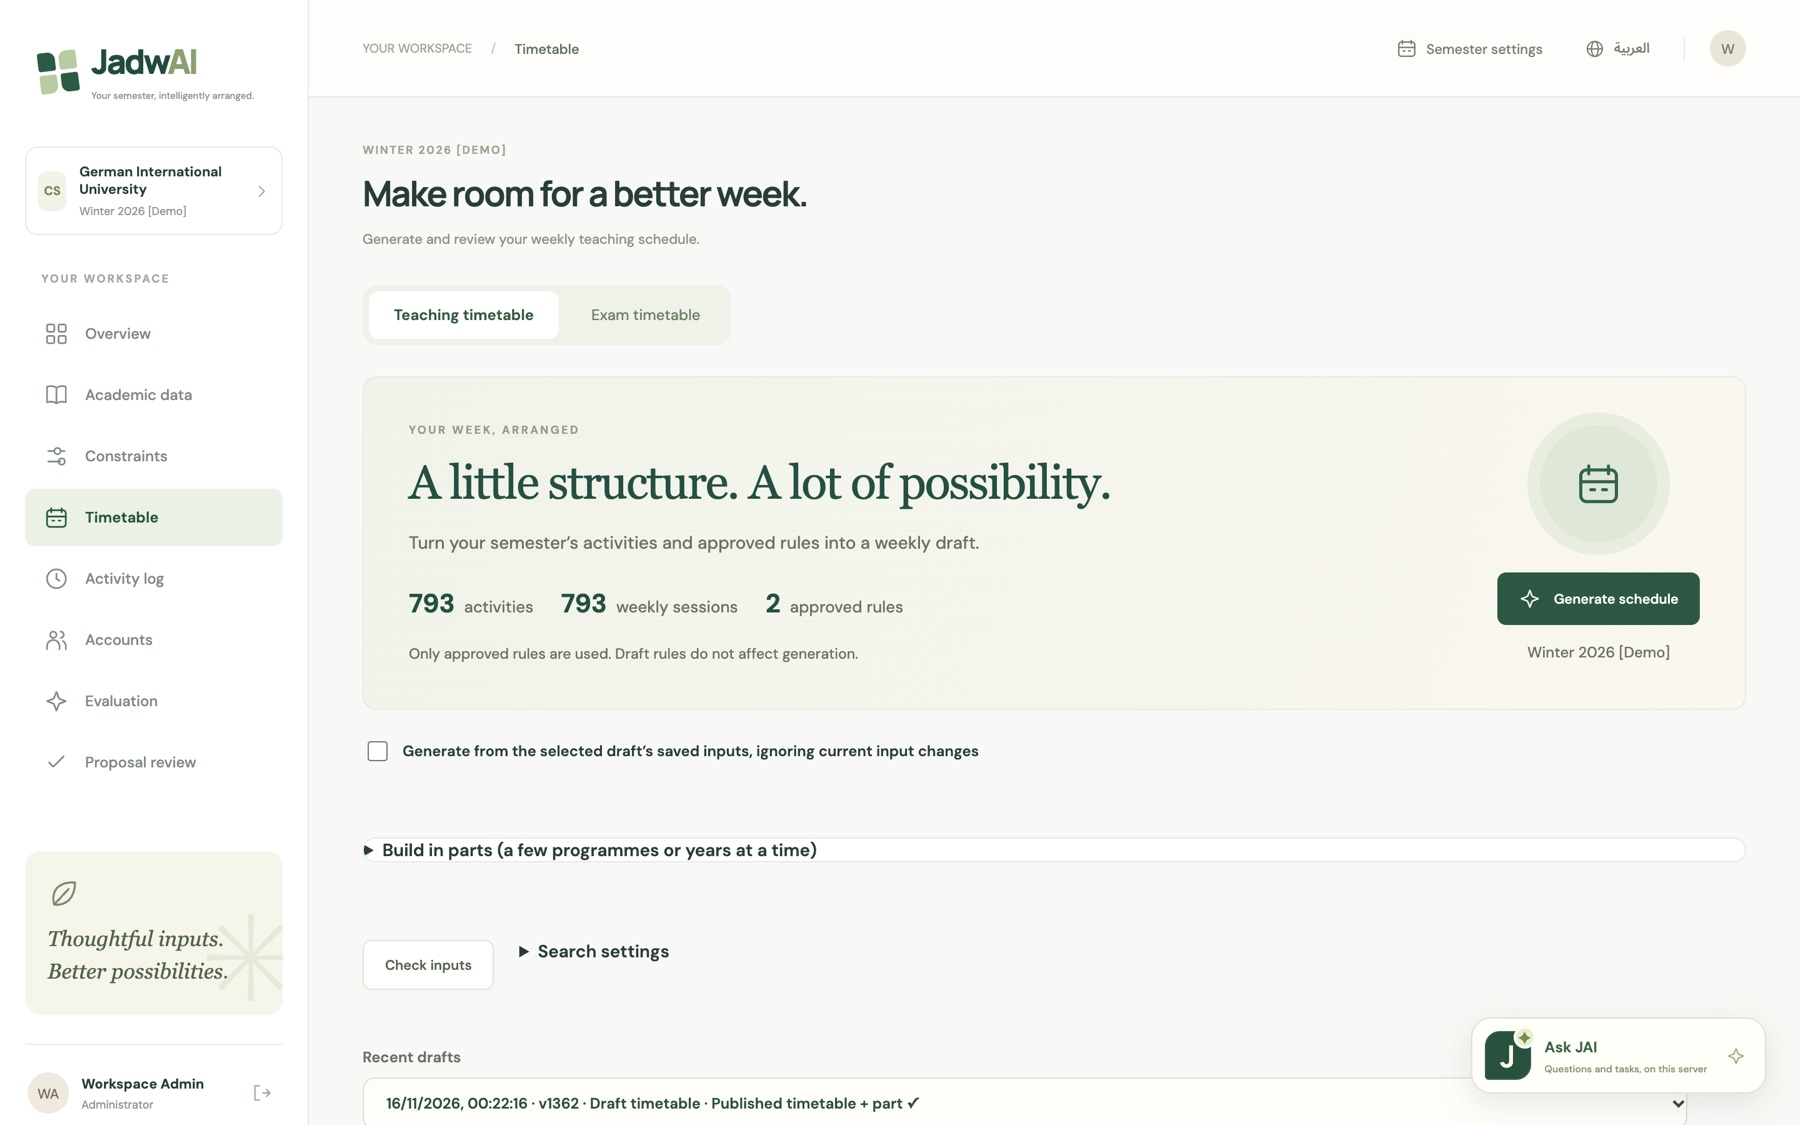
\includegraphics[width=\textwidth]{13-teaching-timetable-top.jpg}
\caption{Teaching timetable: generation from approved rules only, building in parts, input checks, search settings and the list of saved drafts.}
\label{fig:shot-teaching-timetable-top}
\end{figure}

\begin{figure}[p]
\centering
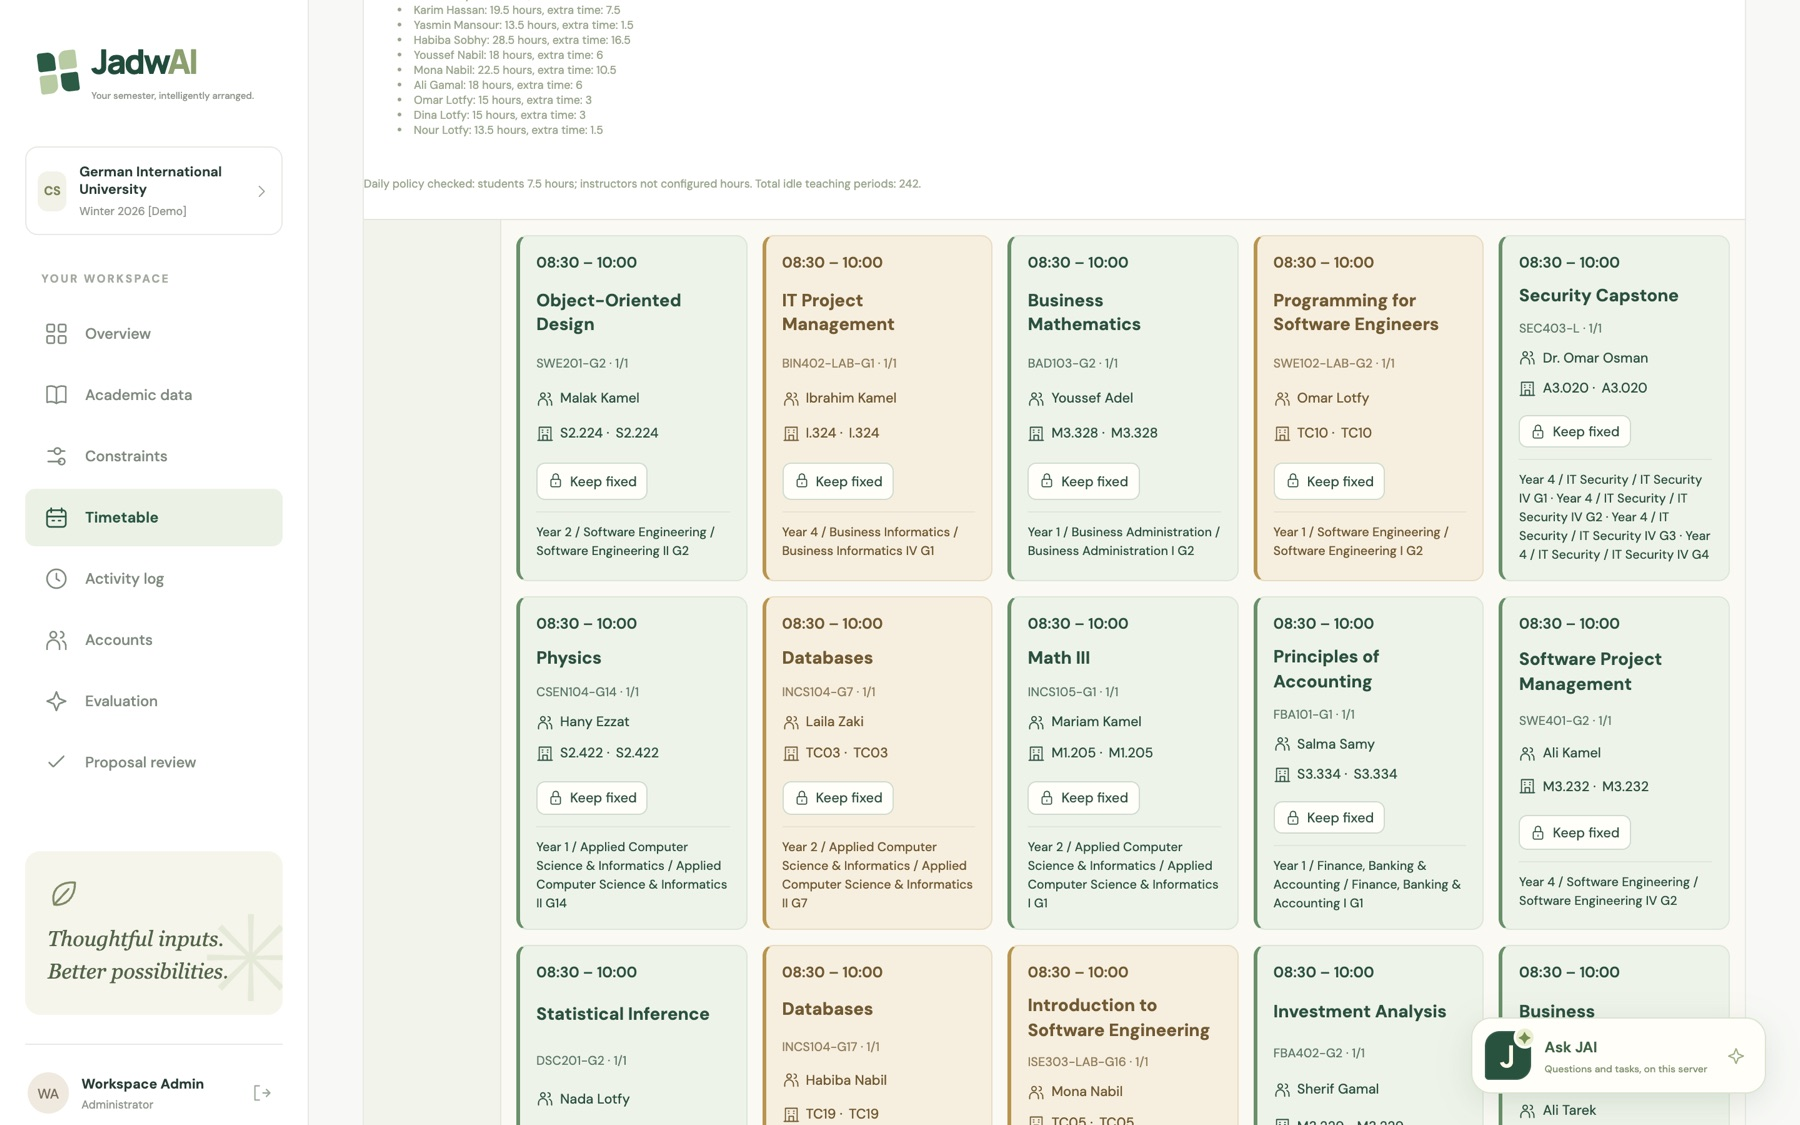
\includegraphics[width=\textwidth]{15-teaching-timetable-2.jpg}
\caption{Part of a published teaching timetable: each session shows time, course, activity, instructor and room, with an option to keep it fixed in later regenerations.}
\label{fig:shot-teaching-timetable-2}
\end{figure}

\begin{figure}[p]
\centering
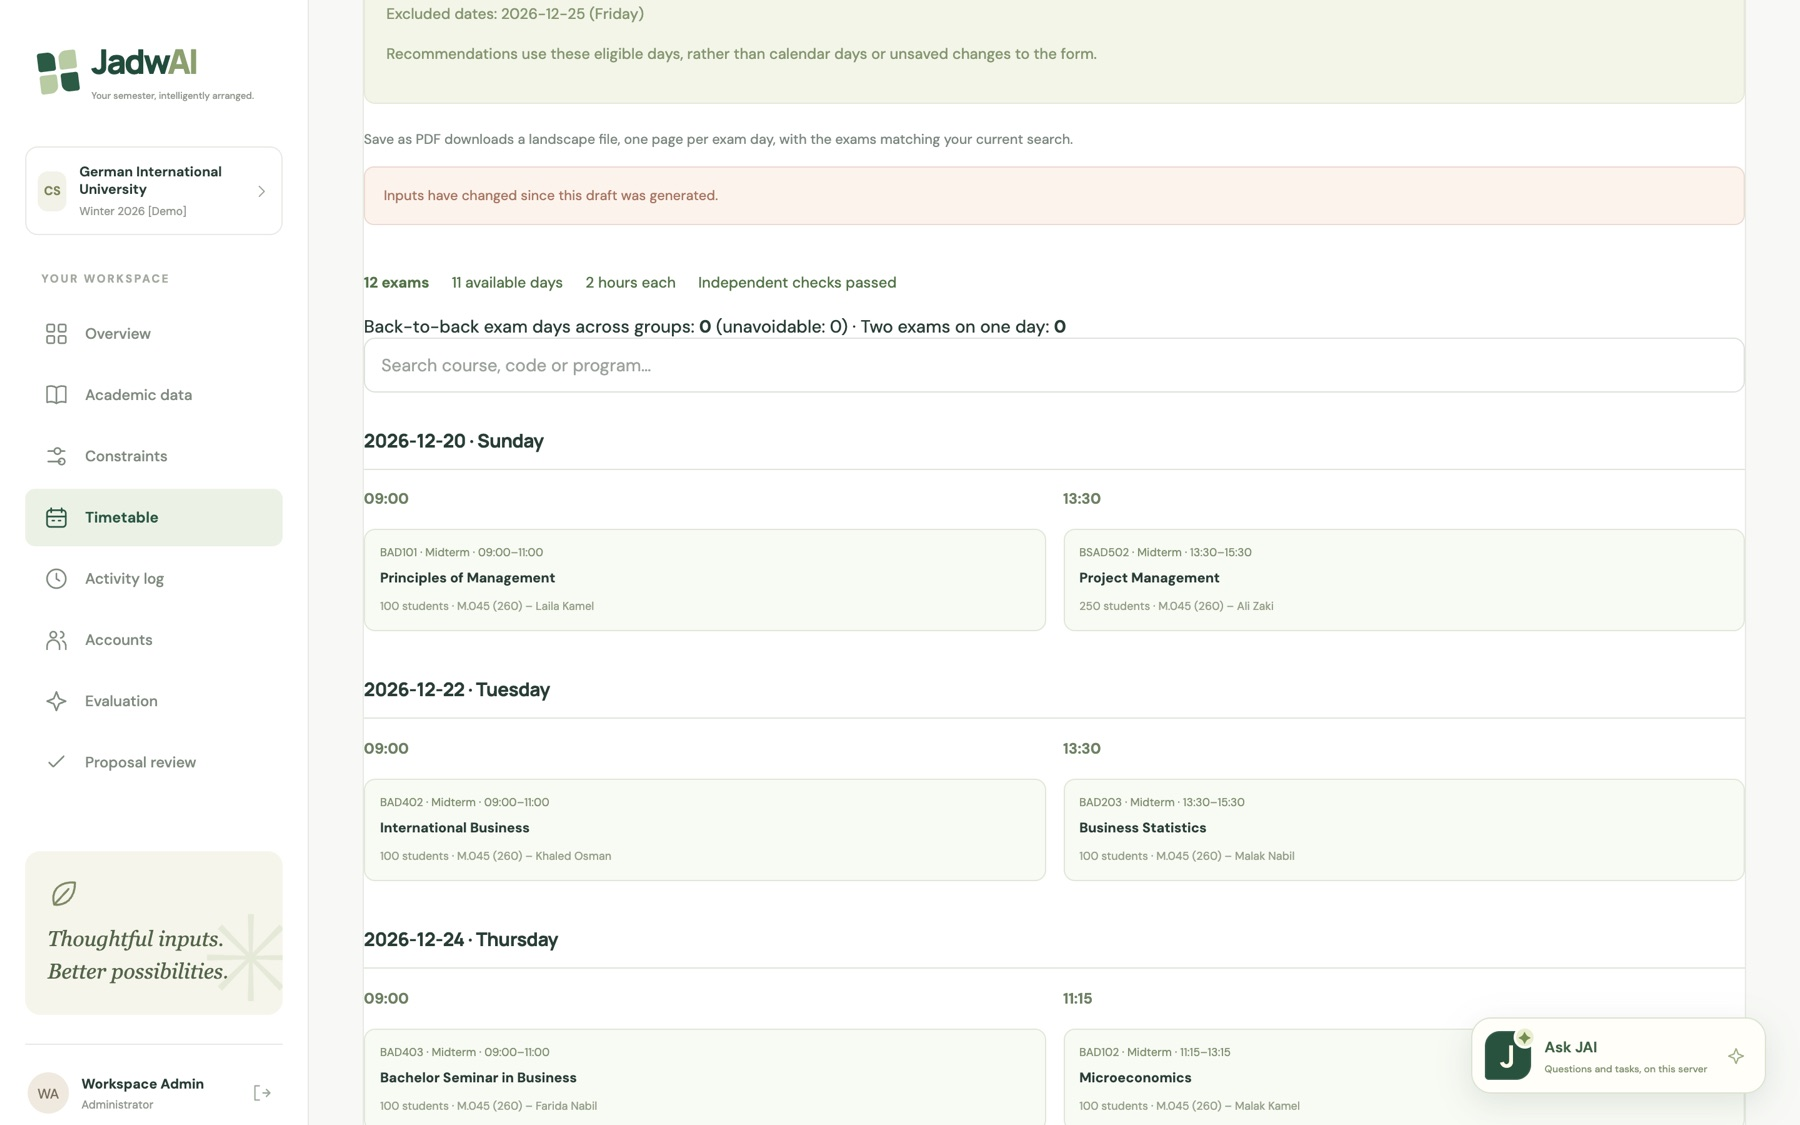
\includegraphics[width=\textwidth]{16-exam-timetable.jpg}
\caption{Examination timetable: midterms by day and time with hall, capacity and invigilator; the summary reports back-to-back examination days across groups.}
\label{fig:shot-exam-timetable}
\end{figure}

\begin{figure}[p]
\centering
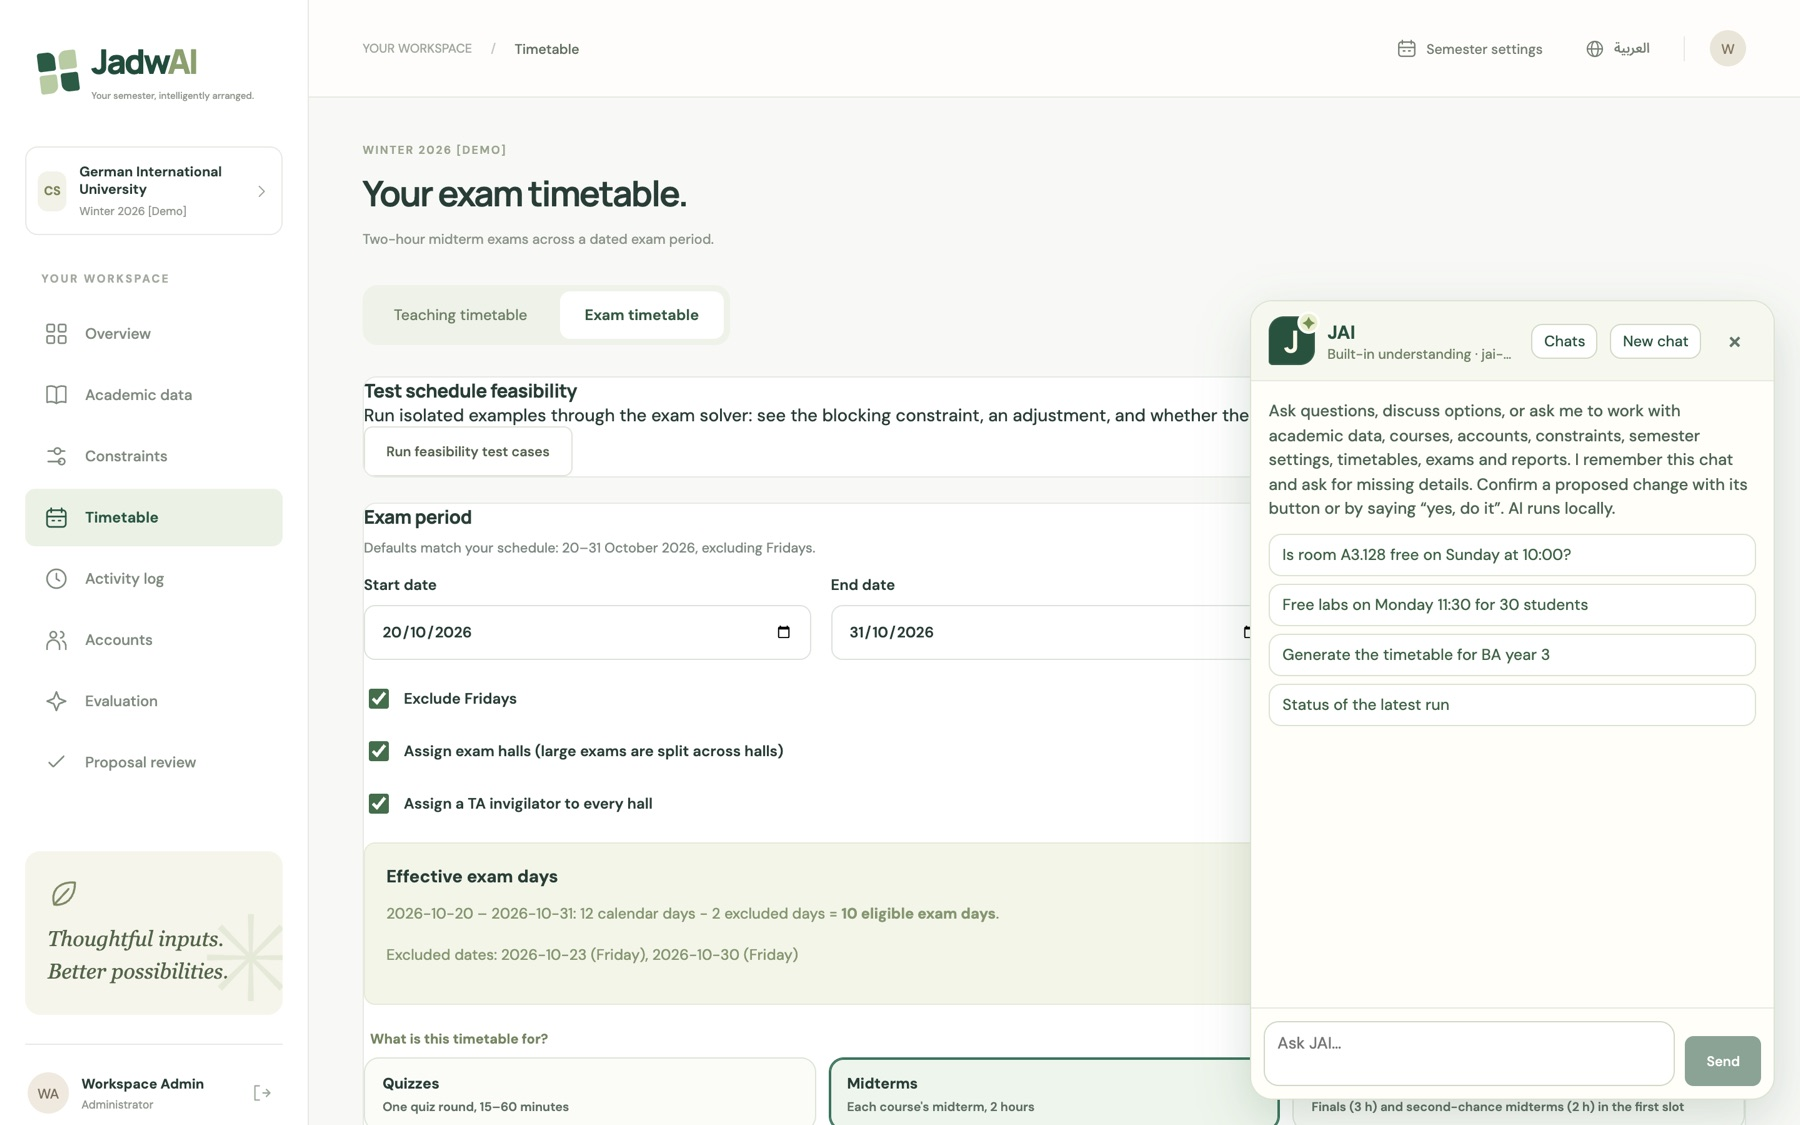
\includegraphics[width=\textwidth]{18-jai-chat.jpg}
\caption{The JAI chat panel beside the exam settings: example questions and tasks; a proposed change runs only after the administrator confirms it.}
\label{fig:shot-jai-chat}
\end{figure}

\begin{figure}[p]
\centering
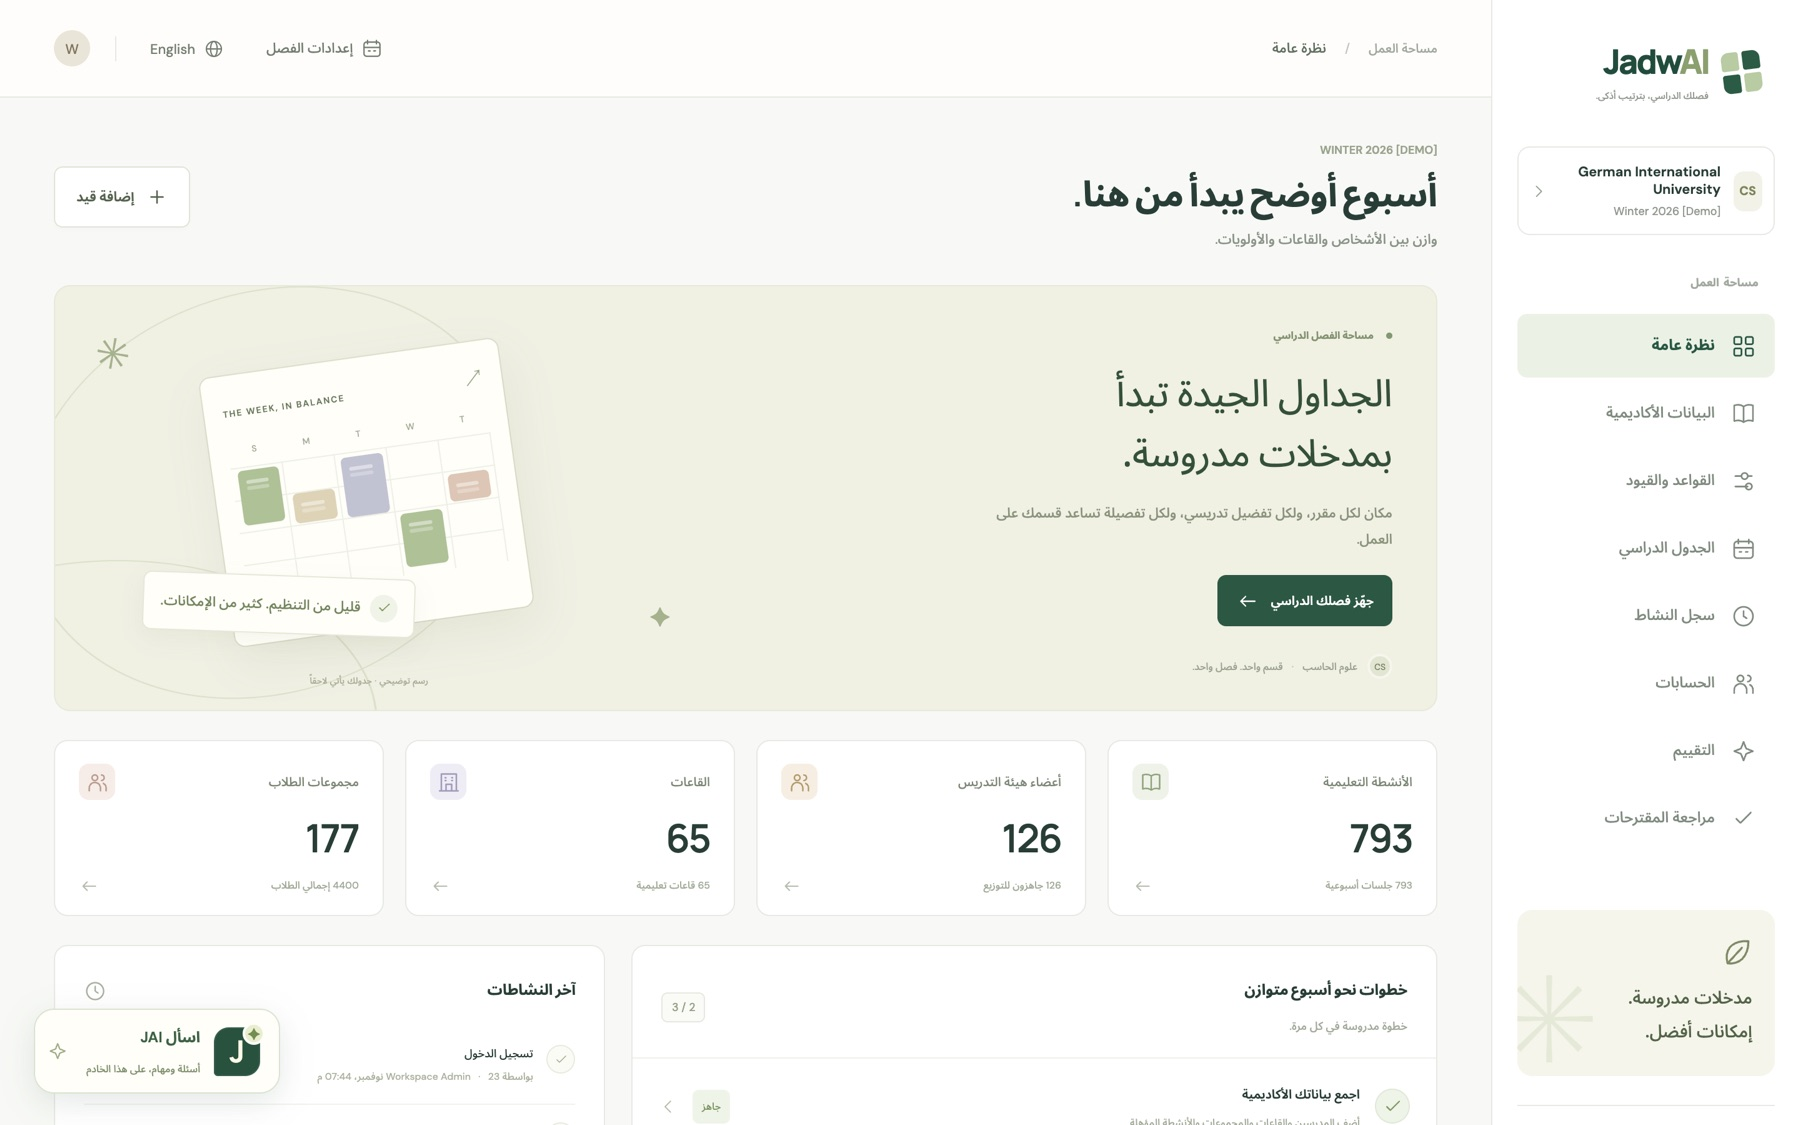
\includegraphics[width=\textwidth]{11-overview-arabic.jpg}
\caption{Arabic interface: the same overview page with right-to-left layout.}
\label{fig:shot-overview-arabic}
\end{figure}

\begin{figure}[p]
\centering
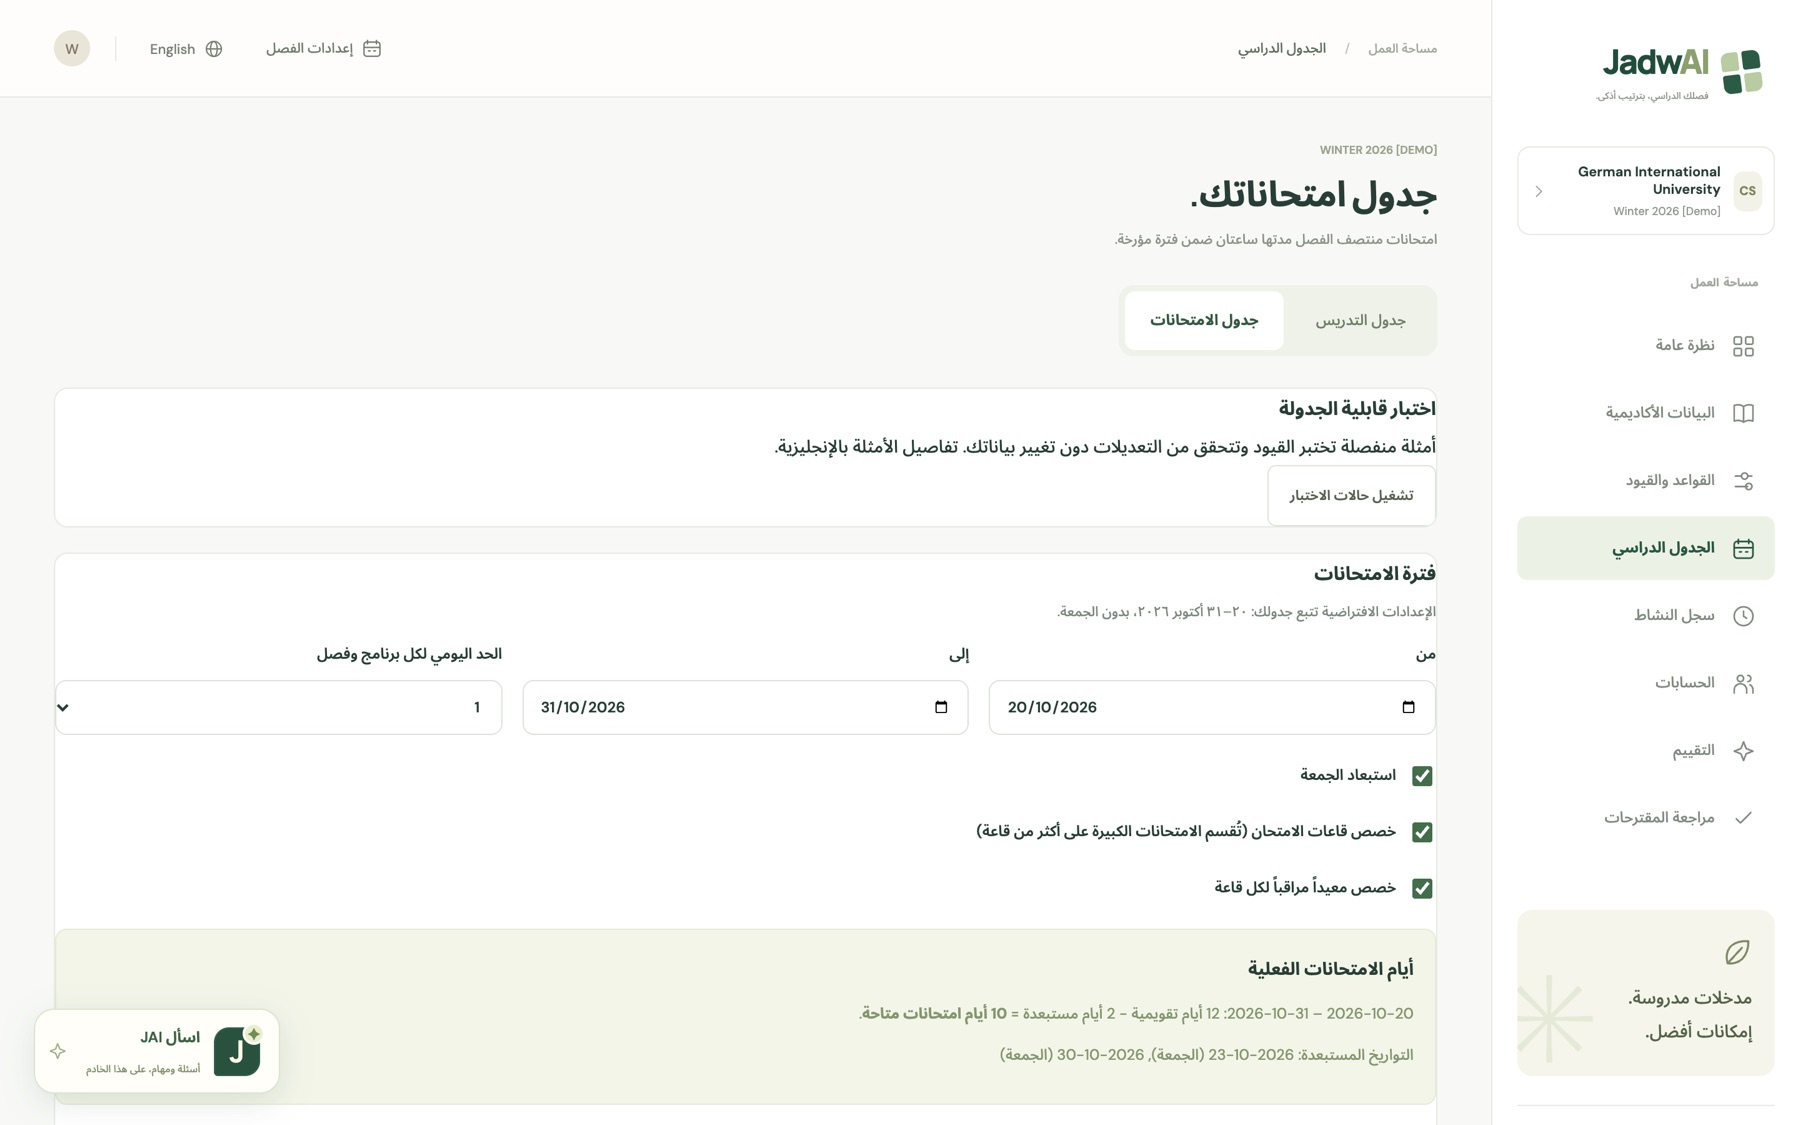
\includegraphics[width=\textwidth]{12-timetable-arabic.jpg}
\caption{Arabic interface: the examination settings page.}
\label{fig:shot-timetable-arabic}
\end{figure}

\clearpage

\chapter{Project Record and Traceability}\label{app:planning}

% NOTE (24 Nov 2026): Replaces the October planning records (timeline without dates, proposed deliverables, open decisions). Drafted with AI assistance; reword in your own words. Dates come from the SRS versions, the corpus manifests, finetuning/RESULTS.md and the git history.

\section{Timeline}\label{timeline}

Table~\ref{tab:timeline} lists the main milestones of the project as they happened.

\begin{longtable}[]{@{}p{0.24\textwidth}p{0.68\textwidth}@{}}
\caption{Project milestones.}\label{tab:timeline}\\
\toprule
Date (2026) & Milestone \\
\midrule
\endhead
\bottomrule
\endlastfoot
10 October & SRS draft v0.2 reviewed by the supervisor \\
25 October & Synthetic corpus release \texttt{0.1.0-draft} (128 statements) and annotation guide v1 \\
1 November & Development bundle \texttt{0.2.0-draft} (144 statements, two contexts) and annotation guide v2 \\
4--8 November & Examination halls and invigilators, scenarios and publication, portals, advising students, generation in parts, repair suggestions \\
8 November & Measured evidence for Chapter~\ref{evidence} (department and university scale, repair, rule-based baseline) \\
12 November & Examination plans with quizzes, midterms, finals and second chances \\
14--18 November & JAI chat: built-in answers, local model, confirmed tasks; SRS v0.4 \\
19--23 November & JAI fine-tuning rounds 1--3, verified guide, blind rating, Arabic reply and display fixes \\
23--24 November & Fine-tuning round 4 and its blind rating; two local-model extraction runs on the development corpus; examination publishing as a built-in chat route; annotation guide v2.1 merges two pairs of synonymous codes; thesis moved to the GIU template \\
10 December & Full draft due to the supervisor \\
\end{longtable}

\section{Deliverables}\label{proposed-deliverables-of-the-study}

\begin{itemize}
\item The JadwAI prototype (\texttt{frontend/}, \texttt{backend/}, \texttt{worker/}) with its automated tests.
\item The requirements with their status (\texttt{docs/REQUIREMENTS.md}, summarised in Appendix~\ref{app:requirements}).
\item The output contract, annotation guides, synthetic corpus and offline scorer (\texttt{evaluation/}).
\item The fine-tuning data, training notebook, merge and evaluation tools, and results (\texttt{finetuning/}).
\item The scripts, logs, predictions and scores behind every reported measurement, in \texttt{thesis/evidence/}.
\item This thesis.
\end{itemize}

\section{Traceability to the requirements}\label{consistency-with-the-srs-traceability}

Table~\ref{tab:trace} links each part of the method in Chapter~\ref{methodology-proposed-study} to the functional requirements it relies on.

\begin{longtable}[]{@{}p{0.5\textwidth}p{0.42\textwidth}@{}}
\caption{Traceability of the method to the requirements.}\label{tab:trace}\\
\toprule
Element of the method & Requirement or procedure \\
\midrule
\endhead
\bottomrule
\endlastfoot
Schema-constrained interpretation & FR-015, FR-022, FR-074 \\
Entity resolution without invented entities & FR-016 \\
Parameters and named periods & FR-001, FR-017, FR-067 \\
Negation and mandatory/preferred strength & FR-018 \\
Clarification and unsupported requests & FR-019 \\
Review beside the original statement & FR-020 \\
Approval gate before generation & FR-021 \\
Rule-based parser compared with the model & FR-073 \\
Four language categories & FR-054 \\
Corpus, scorer and development records & FR-049 \\
Manual entry (forms) & FR-010 \\
Manual versus assisted entry with participants & FR-050 (not carried out) \\
Scheduling measures & FR-024--FR-029, FR-031 \\
Validator checks, coverage and publication gate & FR-030--FR-033, FR-040, FR-063 \\
Repair suggestions & FR-058 \\
Examination timetables & FR-051, FR-071, FR-072 \\
JAI assistant and its evaluation & FR-075--FR-077 \\
Reproducibility records & FR-023--FR-025; NFR-016 \\
Comparison of validator and solver model & NFR-002 (research procedure) \\
Annotator agreement and confidence intervals & Research procedure, no FR \\
\end{longtable}




% IEEE numeric style (numbered in order of first citation); the template default was plain
\bibliographystyle{ieeetr}
\bibliography{references}
\addcontentsline{toc}{chapter}{References}

\end{document}
